%!TEX root = Manuscrit.tex
\chapter{Segmentation sémantique multi-modale}
\label{chap:multimodal}
%\citationChap{Watson, you can see everything. You fail, however, to reason from what you see.}{Sherlock Holmes (Arthur Conan Doyle)}
\minitoc

\chapsummary{%
\lettrine{L}{es} chapitres précédent nous ont permis d'établir de nouveaux états de l'art en segmentation sémantique d'images de télédétection sur l'ensemble des capteurs optiques couramment mise en \oe{}uvre pour l'observation de la Terre. Cependant, nous avons également souligné la difficulté d'exploiter directement les modèles numériques de terrain dérivés du \gls{Lidar}.

Dans ce chapitre, nous étudions les techniques de fusion de données permettant de combiner l'information issue de capteurs hétérogènes. Notamment, nous proposons plusieurs architectures multi-modales pour l'apprentissage profond capables d'apprendre conjointement à partir des images optiques et des modèles numériques de terrain. Nous validons ces modèles avec succès sur plusieurs jeux de données et montrons ainsi qu'il est possible de tirer profit de la complémentarité des différents capteurs.

Nous étendons ensuite ces travaux à des sources de données non physiques. En particulier, nous appliquons ces architectures de fusion de donnée à des connaissances géographiques a priori provenant de bases de données en ligne, afin de consolider les cartes sémantiques prédites par le réseau. En considérant cette source d'information comme un capteur virtuel, les architectures multi-modales précédemment développées nous permettent d'insérer des connaissances préalables dans les processus d'apprentissage et d'inférence de nos réseaux de neurones.
}

\newpage

\section{Apprentissage multi-modal}

\subsection{Réseaux de neurones et apprentissage multi-modal}

\begin{figure}[h]
  \hfill
  \begin{subfigure}[b]{0.43\textwidth}
    \resizebox{\textwidth}{!}{
      \documentclass{standalone}
\usepackage[utf8]{inputenc}
\usepackage[T1]{fontenc}
\usepackage{tikz}
\usepackage{ifthen}
%%%%%%%%%%%%%%%%%%%%%%%%%%%%%%%%%%%%%%%%
%           Commandes perso            %
%%%%%%%%%%%%%%%%%%%%%%%%%%%%%%%%%%%%%%%%

%% Figures centrées, et en position 'here, top, bottom or page'
\newenvironment{figureth}{%
		\begin{figure}[htbp]
			\centering
	}{
		\end{figure}
		}


%% Tableaux centrés, et en position 'here, top, bottom or page'
\newenvironment{tableth}{%
		\begin{table}[htbp]
			\centering
			%\rowcolors{1}{coleurtableau}{coleurtableau}
	}{
		\end{table}
		}

%% Sous-figures centrées, en position 'top'
\newenvironment{subfigureth}[1]{%
	\begin{subfigure}[t]{#1}
	\centering
}{
	\end{subfigure}
}

\newcommand{\citationChap}[2]{%
	\epigraph{\og \textit{#1} \fg{}}{#2}
}

%% On commence par une page impaire quand on change le style de numérotation de pages
\let\oldpagenumbering\pagenumbering
\renewcommand{\pagenumbering}[1]{%
	\cleardoublepage
	\oldpagenumbering{#1}
}

%% Légende du dataset ISPRS
\newcommand\isprslegende{
Légende\,: \textcolor{Black}{blanc}\,: routes, \textcolor{Blue}{bleu}\,: bâtiments, \textcolor{Cerulean}{cyan}\,: végétation basse, \textcolor{OliveGreen}{vert}\,: arbres, \textcolor{Dandelion}{jaune}\,: véhicules, \textcolor{BrickRed}{rouge}\,: autre.
}

%% Dessiner des réseaux de neurones avec Tikz
\newcommand{\convlayer}[9]{%{h}{w}{d}{name}{color}{x}{y}{z}%{note w}{note h}{note d}
   \def\h{#1}
   \def\w{#2}
   \def\d{#3}
   \def\name{#4}
   \ifthenelse {\equal{#5} {}} {\def\col{white}} {\def\col{#5}}
   \def\x{#6}
   \ifthenelse {\equal{#7} {}} {\def\y{0}} {\def\y{#7}}
   \ifthenelse {\equal{#8} {}} {\def\z{0}} {\def\z{#8}}
   % ne faites pas ça chez vous !
   \ifthenelse {\equal{#9} {}} {\convlayercontinued{}{}{}} {\convlayercontinued#9}
}

\newcommand\convlayercontinued[3]{
   \def\notew{#1}
   \def\noteh{#2}
   \def\noted{#3}
   \coordinate (A) at (\x-\d/2,  \y-\h/2, \z-\w/2);
   \coordinate (B) at (\x-\d/2,  \y-\h/2, \z+\w/2);
   \coordinate (C) at (\x-\d/2,  \y+\h/2, \z+\w/2);
   \coordinate (D) at (\x-\d/2,  \y+\h/2, \z-\w/2);
   \coordinate (E) at (\x+\d/2,  \y-\h/2, \z-\w/2);
   \coordinate (F) at (\x+\d/2,  \y-\h/2, \z+\w/2);
   \coordinate (G) at (\x+\d/2,  \y+\h/2, \z+\w/2);
   \coordinate (H) at (\x+\d/2,  \y+\h/2, \z-\w/2);

    \draw [draw opacity=0.3, fill opacity=0.8, fill=\col!60!white] (A) -- (B) -- (C) -- (D) -- cycle;
    \draw [draw opacity=0.3, fill opacity=0.8, fill=\col!60!white] (A) -- (B) -- (F) -- (E) -- cycle;
    % Face haut
    %\draw [left color=\col!60!white, right color=\col!80!white, shading=axis, shading angle=180] (C) -- (D)  -- (H) -- (G) -- cycle;
    \draw [fill opacity=0.9, fill=\col!70!white] (C) -- node[rotate=45,above] {\small \name} (D) -- (H) -- (G) -- cycle;
    %\draw [fill opacity=0.9, fill=\col!70!white] (C) -- (D) -- node[above] {\small \name} (H) -- (G) -- cycle;
    % Face droite
    \draw [fill opacity=0.9, fill=\col!60!white] (E) -- node[pos=0.75,rotate=45,below] {\scriptsize \notew} (F) -- (G) --  (H) -- cycle;
    % Face avant
    %\draw [shading=axis, left color=\col!60!white, right color=\col!40!white, shading angle=-45] (B) -- node[above,rotate=90] {\scriptsize \noteh} (C) -- (G) -- (F) -- node[below] {\scriptsize \noted}  cycle;
    \draw [fill opacity=0.9, fill=\col!50!white] (B) -- node[above,rotate=90] {\scriptsize \noteh} (C) -- (G) -- (F) -- node[below] {\scriptsize \noted}  cycle;
}

\newcommand{\fclayer}[8]{%{h}{w}{name}{color}{x}{y}{z}
   \def\h{#1}
   \def\w{#2}
   \def\name{#3}
   \ifthenelse {\equal{#4} {}} {\def\col{white}} {\def\col{#4}}
   \def\x{#5}
   \def\y{#6}
   \def\z{#7}
   \def\note{#8}
   \coordinate (A) at (\x-\w/2,  \y-\h/2, \z);
   \coordinate (B) at (\x+\w/2,  \y-\h/2, \z);
   \coordinate (C) at (\x+\w/2,  \y+\h/2, \z);
   \coordinate (D) at (\x-\w/2,  \y+\h/2, \z);

   \pgfmathparse{4*\w}\let\boxwidth\pgfmathresult
    \draw [fill=\col] (A) -- node[below,text width=\boxwidth cm,align=center] {\scriptsize \note} (B) -- (C) -- (D) -- cycle;

    \node (N) at ($(A)!0.5!(B)+(0,-1,0)$) {\name};
}

\newcommand{\alexnet}[4]{%{scale}{x}{y}{z}
  \def\scale{#1}
  \def\alexx{#2}
  \def\alexy{#3}
  \def\alexz{#4}


  \def\coblue{blue!50!white}
  \def\fcgrey{gray!50!white}

  \convlayer{1.3*\scale}{1.3*\scale}{0.02*\scale}{Image}{\coblue}{\alexx}{\alexy}{\alexz}{{227}{227}{3}}
  \convlayer{1.1*\scale}{1.1*\scale}{0.08*\scale}{Conv1}{\coblue}{\alexx+0.7*\scale}{\alexy}{\alexz}{{55}{55}{96}}
  \convlayer{0.7*\scale}{0.7*\scale}{0.5*\scale}{Conv2}{\coblue}{\alexx+1.5*\scale}{\alexy}{\alexz}{{27}{27}{256}}
  \convlayer{0.5*\scale}{0.5*\scale}{0.8*\scale}{Conv3}{\coblue}{\alexx+2.6*\scale}{\alexy}{\alexz}{{13}{13}{384}}
  \convlayer{0.5*\scale}{0.5*\scale}{0.8*\scale}{Conv4}{\coblue}{\alexx+3.8*\scale}{\alexy}{\alexz}{{13}{13}{384}}
  \convlayer{0.5*\scale}{0.5*\scale}{0.5*\scale}{Conv5}{\coblue}{\alexx+4.8*\scale}{\alexy}{\alexz}{{13}{13}{256}}
  \fclayer{\scale}{0.1*\scale}{FC1}{\fcgrey}{\alexx+5.4*\scale}{\alexy}{\alexz}{4096}
  \fclayer{\scale}{0.1*\scale}{FC2}{\fcgrey}{\alexx+5.7*\scale}{\alexy}{\alexz}{4096}
  \fclayer{\scale}{0.1*\scale}{FC3}{\fcgrey}{\alexx+6.0*\scale}{\alexy}{\alexz}{1000}
}

\newcommand{\imagelayer}[7]{%{width}{x}{y}{z}{path}{text_up}{text_down}
    \pgfmathparse{#1}\let\w\pgfmathresult
    \begin{scope}[canvas is yz plane at x=#2]
     \node[transform shape] (source) at (#3, #4) {\includegraphics[angle=-90,width=\w cm]{#5}};
    \end{scope}
     \node [transform shape, rotate=45, above] at (source.east) {#6};
     \node [transform shape, rotate=45, below] at (source.west) {\scriptsize{#7}};
}

\def\fourier{\mathcal{F}}

\newcommand{\lightspectrum}{%
\pgfplotsset{
    % this *defines* a custom colormap ...
    colormap={slategraywhite}{color(0cm)=(red); color(1cm)=(red); color(2cm)=(red); color(3cm)=(red); color(4cm)=(orange); color(5cm)=(yellow); color(6cm)=(green); color(7cm)=(blue); color(8cm)=(blue); color(9cm)=(purple); color(10cm)=(purple); color(12cm)=(black)}
}
\node at (1.5, 2.7) {\small 1mm};
\node at (4, 3) {Infrarouge};
\node at (7.75, 2.7) {\small 800nm};
\node at (9, 3) {Visible};
\node at (10.5, 2.7) {\small 400nm};
\node at (12, 3) {Ultraviolet};
\node at (13.5, 2.7) {\small 10nm};
\draw[->] (1, 2.5) -- (14, 2.5);
\begin{axis}[hide axis,width=16cm,height=4cm,colormap name=slategraywhite]
\addplot[domain=20:1000,samples=1500,ultra thick, point meta=x*x,mesh]{sin(x*x/80)};
\end{axis}
}

% Union généralisée
\newcommand{\wbigcup}{\mathop{\bigcup}\displaylimits}

\newcommand{\res}[2]{#1 {\footnotesize $\pm$ #2}}
\newcommand{\bres}[2]{\textbf{#1} {\footnotesize $\pm$ #2}}
\newcommand{\bbres}[2]{\res{\textit{#1}}{#2}}

\newcommand{\drawkernel}[9]{
\begin{tikzpicture}
	\draw[step=1cm,gray!50!white,very thin] (0,0) grid (3,3);
	\kernelnode{0.5}{0.5}{#1};
	\kernelnode{0.5}{1.5}{#2};
	\kernelnode{0.5}{2.5}{#3};
	\kernelnode{1.5}{0.5}{#4};
	\kernelnode{1.5}{1.5}{#5};
	\kernelnode{1.5}{2.5}{#6};
	\kernelnode{2.5}{0.5}{#7};
	\kernelnode{2.5}{1.5}{#8};
	\kernelnode{2.5}{2.5}{#9};
\end{tikzpicture}
}

\newcommand{\kernelnode}[3]{%{x}{y}{value}
	\ifthenelse{\equal{#3}{0}}{
		\def\kcolor{gray}
	}{
		\def\kcolor{black}
	}
	\node[\kcolor] at (#1, #2) {#3};
}

\newcommand{\chapsummary}[1]{
\section*{Résumé du chapitre :}
\parbox{0.9\linewidth}{
\setlength{\parindent}{4ex}
#1}
}

\newcommand{\eqname}[1]{\tag*{\small (#1)}}


\begin{document}
  \begin{tikzpicture}
  \usetikzlibrary{calc}
  \usetikzlibrary{3d}

  \def\scale{3}
  \def\netx{0}
  \def\nety{2}
  \def\netz{0}

  \def\coorange{orange!50!white}
  \def\coblue{blue!50!white}
  \def\cogreen{green!50!white}

  \node[rotate=90] (audio_in) at (0*\scale, \nety) {Entrée audio};
  \draw[->] (audio_in.south) -- (0.425*\scale,\nety);
  \fclayer{\scale}{0.15*\scale}{}{\coorange}{0.5*\scale}{\nety}{\netz}{}
  \draw[->] (0.575*\scale, \nety) -- (0.925*\scale,\nety);
  \fclayer{\scale}{0.15*\scale}{}{\coorange}{1*\scale}{\nety}{\netz}{}

  \node[rotate=90] (audio_out) at (3*\scale, \nety) {Reconstruction audio};
  \draw[->] (2*\scale,\nety) -- (2.425*\scale,\nety);
  \fclayer{\scale}{0.15*\scale}{}{\coorange}{2*\scale}{\nety}{\netz}{}
  \draw[->] (2.5*\scale,\nety) -- (audio_out.north);
  \fclayer{\scale}{0.15*\scale}{}{\coorange}{2.5*\scale}{\nety}{\netz}{}

  
  \fclayer{1.5*\scale}{0.15*\scale}{}{\coblue}{1.5*\scale}{0}{\netz}{Représentation\\ jointe}

  \draw (1.075*\scale,\nety) edge[in=180,out=0,->] (1.425*\scale,0);
  \draw (1.575*\scale,0) edge[in=180,out=0,->] (1.925*\scale,\nety);
  \renewcommand\nety{-2}
  \draw (1.075*\scale,\nety) edge[in=180,out=0,->] (1.425*\scale,0);
  \draw (1.575*\scale,0) edge[in=180,out=0,->] (1.925*\scale,\nety);

  \node[rotate=90] (video_in) at (0*\scale, \nety) {Entrée vidéo};
  \draw[->] (video_in.south) -- (0.425*\scale,\nety);
  \fclayer{\scale}{0.15*\scale}{}{\cogreen}{0.5*\scale}{\nety}{\netz}{}
  \draw[->] (0.575*\scale, \nety) -- (0.925*\scale,\nety);
  \fclayer{\scale}{0.15*\scale}{}{\cogreen}{1*\scale}{\nety}{\netz}{}

  \node[rotate=90] (video_out) at (3*\scale, \nety) {Reconstruction vidéo};
  \draw[->] (2*\scale,\nety) -- (2.425*\scale,\nety);
  \fclayer{\scale}{0.15*\scale}{}{\cogreen}{2*\scale}{\nety}{\netz}{}
  \draw[->] (2.5*\scale,\nety) -- (video_out.north);
  \fclayer{\scale}{0.15*\scale}{}{\cogreen}{2.5*\scale}{\nety}{\netz}{}

  \end{tikzpicture}
\end{document}

    }
    \caption{Auto-encodeur multimodal~\cite{ngiam_multimodal_2011}}
    \label{fig:ae_multimodal}
  \end{subfigure}%
  \hfill
  \begin{subfigure}[b]{0.53\textwidth}
    \resizebox{\textwidth}{!}{
      \documentclass{standalone}
\usepackage[utf8]{inputenc}
\usepackage[T1]{fontenc}
\usepackage{tikz}
\usepackage{ifthen}
%%%%%%%%%%%%%%%%%%%%%%%%%%%%%%%%%%%%%%%%
%           Commandes perso            %
%%%%%%%%%%%%%%%%%%%%%%%%%%%%%%%%%%%%%%%%

%% Figures centrées, et en position 'here, top, bottom or page'
\newenvironment{figureth}{%
		\begin{figure}[htbp]
			\centering
	}{
		\end{figure}
		}


%% Tableaux centrés, et en position 'here, top, bottom or page'
\newenvironment{tableth}{%
		\begin{table}[htbp]
			\centering
			%\rowcolors{1}{coleurtableau}{coleurtableau}
	}{
		\end{table}
		}

%% Sous-figures centrées, en position 'top'
\newenvironment{subfigureth}[1]{%
	\begin{subfigure}[t]{#1}
	\centering
}{
	\end{subfigure}
}

\newcommand{\citationChap}[2]{%
	\epigraph{\og \textit{#1} \fg{}}{#2}
}

%% On commence par une page impaire quand on change le style de numérotation de pages
\let\oldpagenumbering\pagenumbering
\renewcommand{\pagenumbering}[1]{%
	\cleardoublepage
	\oldpagenumbering{#1}
}

%% Légende du dataset ISPRS
\newcommand\isprslegende{
Légende\,: \textcolor{Black}{blanc}\,: routes, \textcolor{Blue}{bleu}\,: bâtiments, \textcolor{Cerulean}{cyan}\,: végétation basse, \textcolor{OliveGreen}{vert}\,: arbres, \textcolor{Dandelion}{jaune}\,: véhicules, \textcolor{BrickRed}{rouge}\,: autre.
}

%% Dessiner des réseaux de neurones avec Tikz
\newcommand{\convlayer}[9]{%{h}{w}{d}{name}{color}{x}{y}{z}%{note w}{note h}{note d}
   \def\h{#1}
   \def\w{#2}
   \def\d{#3}
   \def\name{#4}
   \ifthenelse {\equal{#5} {}} {\def\col{white}} {\def\col{#5}}
   \def\x{#6}
   \ifthenelse {\equal{#7} {}} {\def\y{0}} {\def\y{#7}}
   \ifthenelse {\equal{#8} {}} {\def\z{0}} {\def\z{#8}}
   % ne faites pas ça chez vous !
   \ifthenelse {\equal{#9} {}} {\convlayercontinued{}{}{}} {\convlayercontinued#9}
}

\newcommand\convlayercontinued[3]{
   \def\notew{#1}
   \def\noteh{#2}
   \def\noted{#3}
   \coordinate (A) at (\x-\d/2,  \y-\h/2, \z-\w/2);
   \coordinate (B) at (\x-\d/2,  \y-\h/2, \z+\w/2);
   \coordinate (C) at (\x-\d/2,  \y+\h/2, \z+\w/2);
   \coordinate (D) at (\x-\d/2,  \y+\h/2, \z-\w/2);
   \coordinate (E) at (\x+\d/2,  \y-\h/2, \z-\w/2);
   \coordinate (F) at (\x+\d/2,  \y-\h/2, \z+\w/2);
   \coordinate (G) at (\x+\d/2,  \y+\h/2, \z+\w/2);
   \coordinate (H) at (\x+\d/2,  \y+\h/2, \z-\w/2);

    \draw [draw opacity=0.3, fill opacity=0.8, fill=\col!60!white] (A) -- (B) -- (C) -- (D) -- cycle;
    \draw [draw opacity=0.3, fill opacity=0.8, fill=\col!60!white] (A) -- (B) -- (F) -- (E) -- cycle;
    % Face haut
    %\draw [left color=\col!60!white, right color=\col!80!white, shading=axis, shading angle=180] (C) -- (D)  -- (H) -- (G) -- cycle;
    \draw [fill opacity=0.9, fill=\col!70!white] (C) -- node[rotate=45,above] {\small \name} (D) -- (H) -- (G) -- cycle;
    %\draw [fill opacity=0.9, fill=\col!70!white] (C) -- (D) -- node[above] {\small \name} (H) -- (G) -- cycle;
    % Face droite
    \draw [fill opacity=0.9, fill=\col!60!white] (E) -- node[pos=0.75,rotate=45,below] {\scriptsize \notew} (F) -- (G) --  (H) -- cycle;
    % Face avant
    %\draw [shading=axis, left color=\col!60!white, right color=\col!40!white, shading angle=-45] (B) -- node[above,rotate=90] {\scriptsize \noteh} (C) -- (G) -- (F) -- node[below] {\scriptsize \noted}  cycle;
    \draw [fill opacity=0.9, fill=\col!50!white] (B) -- node[above,rotate=90] {\scriptsize \noteh} (C) -- (G) -- (F) -- node[below] {\scriptsize \noted}  cycle;
}

\newcommand{\fclayer}[8]{%{h}{w}{name}{color}{x}{y}{z}
   \def\h{#1}
   \def\w{#2}
   \def\name{#3}
   \ifthenelse {\equal{#4} {}} {\def\col{white}} {\def\col{#4}}
   \def\x{#5}
   \def\y{#6}
   \def\z{#7}
   \def\note{#8}
   \coordinate (A) at (\x-\w/2,  \y-\h/2, \z);
   \coordinate (B) at (\x+\w/2,  \y-\h/2, \z);
   \coordinate (C) at (\x+\w/2,  \y+\h/2, \z);
   \coordinate (D) at (\x-\w/2,  \y+\h/2, \z);

   \pgfmathparse{4*\w}\let\boxwidth\pgfmathresult
    \draw [fill=\col] (A) -- node[below,text width=\boxwidth cm,align=center] {\scriptsize \note} (B) -- (C) -- (D) -- cycle;

    \node (N) at ($(A)!0.5!(B)+(0,-1,0)$) {\name};
}

\newcommand{\alexnet}[4]{%{scale}{x}{y}{z}
  \def\scale{#1}
  \def\alexx{#2}
  \def\alexy{#3}
  \def\alexz{#4}


  \def\coblue{blue!50!white}
  \def\fcgrey{gray!50!white}

  \convlayer{1.3*\scale}{1.3*\scale}{0.02*\scale}{Image}{\coblue}{\alexx}{\alexy}{\alexz}{{227}{227}{3}}
  \convlayer{1.1*\scale}{1.1*\scale}{0.08*\scale}{Conv1}{\coblue}{\alexx+0.7*\scale}{\alexy}{\alexz}{{55}{55}{96}}
  \convlayer{0.7*\scale}{0.7*\scale}{0.5*\scale}{Conv2}{\coblue}{\alexx+1.5*\scale}{\alexy}{\alexz}{{27}{27}{256}}
  \convlayer{0.5*\scale}{0.5*\scale}{0.8*\scale}{Conv3}{\coblue}{\alexx+2.6*\scale}{\alexy}{\alexz}{{13}{13}{384}}
  \convlayer{0.5*\scale}{0.5*\scale}{0.8*\scale}{Conv4}{\coblue}{\alexx+3.8*\scale}{\alexy}{\alexz}{{13}{13}{384}}
  \convlayer{0.5*\scale}{0.5*\scale}{0.5*\scale}{Conv5}{\coblue}{\alexx+4.8*\scale}{\alexy}{\alexz}{{13}{13}{256}}
  \fclayer{\scale}{0.1*\scale}{FC1}{\fcgrey}{\alexx+5.4*\scale}{\alexy}{\alexz}{4096}
  \fclayer{\scale}{0.1*\scale}{FC2}{\fcgrey}{\alexx+5.7*\scale}{\alexy}{\alexz}{4096}
  \fclayer{\scale}{0.1*\scale}{FC3}{\fcgrey}{\alexx+6.0*\scale}{\alexy}{\alexz}{1000}
}

\newcommand{\imagelayer}[7]{%{width}{x}{y}{z}{path}{text_up}{text_down}
    \pgfmathparse{#1}\let\w\pgfmathresult
    \begin{scope}[canvas is yz plane at x=#2]
     \node[transform shape] (source) at (#3, #4) {\includegraphics[angle=-90,width=\w cm]{#5}};
    \end{scope}
     \node [transform shape, rotate=45, above] at (source.east) {#6};
     \node [transform shape, rotate=45, below] at (source.west) {\scriptsize{#7}};
}

\def\fourier{\mathcal{F}}

\newcommand{\lightspectrum}{%
\pgfplotsset{
    % this *defines* a custom colormap ...
    colormap={slategraywhite}{color(0cm)=(red); color(1cm)=(red); color(2cm)=(red); color(3cm)=(red); color(4cm)=(orange); color(5cm)=(yellow); color(6cm)=(green); color(7cm)=(blue); color(8cm)=(blue); color(9cm)=(purple); color(10cm)=(purple); color(12cm)=(black)}
}
\node at (1.5, 2.7) {\small 1mm};
\node at (4, 3) {Infrarouge};
\node at (7.75, 2.7) {\small 800nm};
\node at (9, 3) {Visible};
\node at (10.5, 2.7) {\small 400nm};
\node at (12, 3) {Ultraviolet};
\node at (13.5, 2.7) {\small 10nm};
\draw[->] (1, 2.5) -- (14, 2.5);
\begin{axis}[hide axis,width=16cm,height=4cm,colormap name=slategraywhite]
\addplot[domain=20:1000,samples=1500,ultra thick, point meta=x*x,mesh]{sin(x*x/80)};
\end{axis}
}

% Union généralisée
\newcommand{\wbigcup}{\mathop{\bigcup}\displaylimits}

\newcommand{\res}[2]{#1 {\footnotesize $\pm$ #2}}
\newcommand{\bres}[2]{\textbf{#1} {\footnotesize $\pm$ #2}}
\newcommand{\bbres}[2]{\res{\textit{#1}}{#2}}

\newcommand{\drawkernel}[9]{
\begin{tikzpicture}
	\draw[step=1cm,gray!50!white,very thin] (0,0) grid (3,3);
	\kernelnode{0.5}{0.5}{#1};
	\kernelnode{0.5}{1.5}{#2};
	\kernelnode{0.5}{2.5}{#3};
	\kernelnode{1.5}{0.5}{#4};
	\kernelnode{1.5}{1.5}{#5};
	\kernelnode{1.5}{2.5}{#6};
	\kernelnode{2.5}{0.5}{#7};
	\kernelnode{2.5}{1.5}{#8};
	\kernelnode{2.5}{2.5}{#9};
\end{tikzpicture}
}

\newcommand{\kernelnode}[3]{%{x}{y}{value}
	\ifthenelse{\equal{#3}{0}}{
		\def\kcolor{gray}
	}{
		\def\kcolor{black}
	}
	\node[\kcolor] at (#1, #2) {#3};
}

\newcommand{\chapsummary}[1]{
\section*{Résumé du chapitre :}
\parbox{0.9\linewidth}{
\setlength{\parindent}{4ex}
#1}
}

\newcommand{\eqname}[1]{\tag*{\small (#1)}}


\begin{document}
  \begin{tikzpicture}
  \usetikzlibrary{calc}
  \usetikzlibrary{3d}

  \def\scale{3}
  \def\alexx{0}
  \def\alexy{3}
  \def\alexz{0}

  \newcommand\basenet[3]{
  \imagelayer{1.3*\scale}{\alexx}{\alexy}{\alexz}{#3}{#2}{3}
  %\convlayer{1.3*\scale}{1.3*\scale}{0.02*\scale}{#2}{#1}{\alexx}{\alexy}{\alexz}{{227}{227}{3}}
  \convlayer{1.1*\scale}{1.1*\scale}{0.1*\scale}{Conv1}{#1}{\alexx+0.6*\scale}{\alexy}{\alexz}{{}{}{96}}
  \convlayer{0.7*\scale}{0.7*\scale}{0.4*\scale}{Conv2}{#1}{\alexx+1.3*\scale}{\alexy}{\alexz}{{}{}{256}}
  \convlayer{0.5*\scale}{0.5*\scale}{0.6*\scale}{Conv3}{#1}{\alexx+2.15*\scale}{\alexy}{\alexz}{{}{}{384}}
  \convlayer{0.5*\scale}{0.5*\scale}{0.6*\scale}{Conv4}{#1}{\alexx+3.05*\scale}{\alexy}{\alexz}{{}{}{384}}
  \convlayer{0.5*\scale}{0.5*\scale}{0.4*\scale}{Conv5}{#1}{\alexx+3.9*\scale}{\alexy}{\alexz}{{}{}{256}}
  \fclayer{\scale}{0.1*\scale}{FC1}{#1}{\alexx+4.4*\scale}{\alexy}{\alexz}{4096}
  \fclayer{\scale}{0.1*\scale}{FC2}{#1}{\alexx+4.7*\scale}{\alexy}{\alexz}{4096}
  }


  \def\coblue{blue!50!gray}
  \def\cogreen{green!50!gray}
  \def\fcgrey{gray!80!white}

  \basenet{\coblue}{Image}{eitel_rgb}
  \renewcommand\alexy{-3}
  \basenet{\cogreen}{Profondeur}{eitel_depth}


  \fclayer{2*\scale}{0.1*\scale}{Fusion}{\fcgrey}{\alexx+5.1*\scale}{0}{\alexz}{4096}
  \fclayer{2*\scale}{0.1*\scale}{}{\fcgrey}{\alexx+5.4*\scale}{0}{\alexz}{51}

  \end{tikzpicture}
\end{document}

    }
    \caption{\glsname{CNN} multimodal~\cite{eitel_multimodal_2015}}
    \label{fig:cnn_multimodal}
  \end{subfigure}
  \hfill
\end{figure}

Jusqu'à présent nous n'avons présenté que des réseaux de neurones n'opérant que sur un seul type de données. Toutefois, la perception sensorielle humaine mobilise plusieurs modalités, notamment le son et l'image, présentant des interactions entre elles. Une question naturelle est donc de chercher à savoir dans quelle mesure une machine est en mesure d'exploiter ce type d'informations contenues sous plusieurs formes, partiellement redondantes.

Cette question relève de l'apprentissage multi-modal et n'est pas spécifique au domaine de la télédétection. L'apprentissage de représentations à partir de signaux de natures hétérogènes est en effet un domaine de recherche à part entière. \citet{baltrusaitis_multimodal_2017} proposent la taxonomie suivante, dans laquelle les représentations peuvent être conjointes (une même représentation pour plusieurs modalités) ou coordonnées (chaque modalité à une représentation)\,:
\begin{itemize}
    \item Représentation\,: génération de caractéristiques exploitant la complémentarité et la redondance de modalités multiples.
    \item Traduction\,: conversion d'une modalité à une autre.
    \item Alignement\,: identification de correspondances entre une représentation d'une modalité et une autre.
    \item Fusion\,: utilisation en compte plusieurs modalités pour la prise de décision.
\end{itemize}

Un modèle capable de synthétiser l'information visuelle et sonore d'une vidéo pour y assigner des étiquettes peut ainsi fonctionner de plusieurs façons. Une première possibilité est d'extraire des caractéristiques séparément pour le son et l'image puis d'utiliser un classifieur qui travaillera sur les caractéristiques concaténées (fusion). Il est également possible de contraindre les représentations audio et vidéo à respecter des critères de proximité sémantique (alignement) par des mesures de similarité. À l'inverse, une des modalités peut servir de référence à des algorithmes d'adaptation de domaine permettant de projecter une caractéristique audio vers une caractéristique image et inversement (traduction). Enfin, plutôt que de manipuler les représentations séparément, il est possible de construire un modèle travaillant sur des données hétérogènes pour construire une représentation multi-modale unique (représentation).

De nombreuses tâches sont liées à l'apprentissage multi-modal, comme le sous-titrage automatique d'images~\cite{karpathy_deep_2015}, la classification de vidéos~\cite{kim_deep_2013} ou la reconnaissance d'activités à partir de signaux issus de bracelets connectés~\cite{ordonez_deep_2016}. De nombreux jeux de données multi-modaux ont été proposés pour une grande variété de tâches\,: description automatique d'images~\cite{hodosh_framing_2013}, diagnostic médical à partir de scanners variés~\cite{menze_multimodal_2015}, reconnaissance d'action à partir de données 3D et d'images~\cite{ofli_berkeley_2013}, analyse d'émotions ressenties à partir de vidéos~\cite{schuller_avec_2011}, éventuellement enrichie par des mesures cardiaques et neurales~\cite{ringeval_introducing_2013}.

Une des premières méthodes développées pour l'apprentissage multi-modal s'intéresse à la fusion dite tardive, s'appliquant au moment de la prise de décision finale. Dans le cas le plus simple, il s'agit d'utiliser un modèle pour chaque modalité et d'appliquer des méthodes d'apprentissage par ensemble, ou plus directement une combinaison linéaire, pour prendre la décision en tenant compte des entrées hétérogènes. C'est par exemple l'approche retenue par~\citet{yuhas_integration_1989} et~\citet{meier_adaptive_1996} pour la reconnaissance automatique de syllabes à partir de vidéos. On retrouve régulièrement ce type d'approche dans la littérature récente pour le traitement de vidéos, par exemple dans~\cite{noda_audio-visual_2015} qui utilise une chaîne de Markov cachée pour la reconnaissance automatique de la parole.

Toutefois, l'apprentissage profond puise sa force dans l'expressivité des représentations que les modèles peuvent apprendre. Ainsi, l'apprentissage multi-modal profond s'est intéressé à l'étude de caractéristiques conjointes sur des sources de données hétérogènes. \citet{ngiam_multimodal_2011} se sont par exemple intéressés à la construction d'un \gls{DBN} auto-encodeur bi-modal audio-image. Deux encodeurs traitent chaque canal séparément et convergent vers une représentation partagée. Deux décodeurs doivent reconstruire chacun une des modalités à partir de la même représentation, comme illustré dans la~\cref{fig:ae_multimodal}. Un point particulièrement intéressant est que cette représentation partagée se montre capable de compenser la perte d'une modalité. Leur modèle peut ainsi être utilisé pour prédire un phonème à partir de la vidéo seulement ou de l'audio seulement.
\citet{srivastava_multimodal_2014} proposent une architecture similaire conçue à partir de machines de Boltzmann profondes pouvant s'appliquer aux vidéos, mais aussi à des données très hétérogènes comme l'image (signal brut) et des étiquettes descriptives (langage symbolique). Leur modèle permet en outre de générer l'une des modalités à partir de l'autre lorsqu'elle est manquante. Plus récemment, \citet{simonyan_two-stream_2014} introduisent des réseaux à double flux pour la reconnaissance d'action dans des vidéos à partir des modalités son et image.

Récemment, la communauté vision s'est intéressée à la fusion entre images \gls{RVB} et cartes de profondeur pour traiter des données 2,5D, notamment avec l'émergence de capteurs à bas coût permettant l'acquisition de celles-ci, comme le Kinect. S'il est possible de concaténer des caractéristiques issues de modèles pré-entraînés pour générer des représentations multi-modales artificielles~\cite{schwarz_rgb-d_2015,lagrange_benchmarking_2015}, il semble ainsi intéressant de chercher à automatiquement apprendre des représentations conjointes exploitant la complémentarité des sources de données. \citet{eitel_multimodal_2015,guo_two-stream_2016,song_combining_2017} s'inspirent de fait du modèle de~\citet{ngiam_multimodal_2011} en utilisant deux \gls{CNN} en parallèle extrayant des caractéristiques qui sont fusionnées dans une représentation conjointe par les dernières couches, leur permettant ainsi de réaliser directement des classifications d'images \gls{RGB-D}. Cette architecture est illustrée dans la~\cref{fig:cnn_multimodal}. Concrètement, deux réseaux AlexNet en parallèle sont utilisés pour extraire des caractéristiques sur l'image \gls{RVB} et sur une carte de profondeur encodée sur 3 canaux. Les caractéristiques extraites par les couches convolutives d'AlexNet convergent de la même façon que chez~\cite{ngiam_multimodal_2011} et sont utilisées comme entrée du classifieur entièrement connecté commun aux deux réseaux. Ces approches permettent d'améliorer les performances de classifieurs convolutifs par rapport au travail sur l'image \gls{RVB} seule, l'information de profondeur permettant de discriminer certains objets en incluant l'\emph{a priori} géométrique et en permettant diminuer l'influence des occlusions. Ces résultats viennent renforcer ceux obtenus par \citet{simonyan_two-stream_2014} dans lequel un réseau à deux flux pour la classification de vidéos était entraîné en simultané sur chaque image instantanée et sur le flot optique entre deux images successives.

L'architecture FuseNet introduite par~\citet{hazirbas_fusenet_2016} est une extension naturelle de cette approche à la segmentation sémantique. Toujours appliqué sur des images \gls{RGB-D}, FuseNet dérive du modèle SegNet~\cite{badrinarayanan_segnet_2017} présenté dans le~\cref{chap:cartographie}. Deux encodeurs réalisent une extraction de caractéristiques dense sur l'image \gls{RVB} et la carte de profondeur encodée sur 3 canaux. Un décodeur unique réalise le surréchantillonnage et la classification en simultané. Cette méthode permet à \citet{hazirbas_fusenet_2016} d'établir un nouvel état de l'art sur le jeu de données SUN RGB-D, dédié à la segmentation sémantique d'images \gls{RGB-D} en intérieur. \citet{guerry_look_2017} obtiennent également d'excellents résultats en détection de personnes dans des images \gls{RGB-D} en utilisant ces méchanismes d'apprentissage bi-modaux au sein desquels les encodeurs parallèles s'échangent de l'information issue de capteurs complémentaires. Finalement, \citet{lee_rdfnet_2017} proposent une amélioration de cette architecture en l'adaptant au paradigme de l'apprentissage résiduel et établissent à leur tour un nouvel état de l'art sur le jeu de données SUN RGB-D.

Il est intéressant de constater que ces méthodes d'interprétation d'images \gls{RGB-D} traitent toutes séparément les aspects de couleur et de profondeur. En effet, comme pour le multispectral, il est intéressant de pouvoir bénéficier des modèles pré-entraînés forts sur les images \gls{RVB}. Concaténer la carte de profondeur à l'image couleur pour former un tenseur à 4 canaux résulte ainsi en des performances plus faibles qu'en traitant les données séparément.

\subsection{Transposition à la télédétection}

En télédétection, l'utilisation des modèles numériques de terrain pour améliorer les performances des classifieurs image a également été fortement étudiée. Le problème est en effet très similaire à celui de l'interprétation d'images 2,5D \gls{RGB-D}, le \gls{MNT} jouant un rôle très similaire à celui des carte de profondeur.

Toutefois, la plupart des travaux antérieurs à cette thèse ont utilisé des stratégies \emph{ad hoc} pour réaliser cette fusion. \citet{lagrange_benchmarking_2015} concatènent simplement les caractéristiques extraites par des réseaux pré-entraînés pour optimiser un nouveau classifieur \gls{SVM} et \citet{paisitkriangkrai_effective_2015} font de même avec des forêts aléatoires en y intégrant en sus des caractéristiques expertes. Plus récemment, \cite{liu_dense_2017} utilise ces mêmes caractéristiques mais les injectent dans un modèle graphique de type \gls{CRF} pour combiner segmentation sémantique issue d'un \gls{FCN}, modèle de terrain et \gls{NDVI}.

Dans cette thèse, nous étudions des approches profondes de bout en bout n'utilisant ni modèle graphique, ni caractéristiques \emph{ad hoc}. Dans un premier temps, nous nous intéresserons à la fusion optique/\glslink{MNT}{modèle numérique de terrain}, puis nous chercherons comment utiliser ces méthodes pour l'intégration de connaissances \emph{a priori}.

\begin{figure}[h]
    \resizebox{\textwidth}{!}{\documentclass{standalone}
\usepackage{tikz}
\usepackage{ifthen}
%%%%%%%%%%%%%%%%%%%%%%%%%%%%%%%%%%%%%%%%
%           Commandes perso            %
%%%%%%%%%%%%%%%%%%%%%%%%%%%%%%%%%%%%%%%%

%% Figures centrées, et en position 'here, top, bottom or page'
\newenvironment{figureth}{%
		\begin{figure}[htbp]
			\centering
	}{
		\end{figure}
		}


%% Tableaux centrés, et en position 'here, top, bottom or page'
\newenvironment{tableth}{%
		\begin{table}[htbp]
			\centering
			%\rowcolors{1}{coleurtableau}{coleurtableau}
	}{
		\end{table}
		}

%% Sous-figures centrées, en position 'top'
\newenvironment{subfigureth}[1]{%
	\begin{subfigure}[t]{#1}
	\centering
}{
	\end{subfigure}
}

\newcommand{\citationChap}[2]{%
	\epigraph{\og \textit{#1} \fg{}}{#2}
}

%% On commence par une page impaire quand on change le style de numérotation de pages
\let\oldpagenumbering\pagenumbering
\renewcommand{\pagenumbering}[1]{%
	\cleardoublepage
	\oldpagenumbering{#1}
}

%% Légende du dataset ISPRS
\newcommand\isprslegende{
Légende\,: \textcolor{Black}{blanc}\,: routes, \textcolor{Blue}{bleu}\,: bâtiments, \textcolor{Cerulean}{cyan}\,: végétation basse, \textcolor{OliveGreen}{vert}\,: arbres, \textcolor{Dandelion}{jaune}\,: véhicules, \textcolor{BrickRed}{rouge}\,: autre.
}

%% Dessiner des réseaux de neurones avec Tikz
\newcommand{\convlayer}[9]{%{h}{w}{d}{name}{color}{x}{y}{z}%{note w}{note h}{note d}
   \def\h{#1}
   \def\w{#2}
   \def\d{#3}
   \def\name{#4}
   \ifthenelse {\equal{#5} {}} {\def\col{white}} {\def\col{#5}}
   \def\x{#6}
   \ifthenelse {\equal{#7} {}} {\def\y{0}} {\def\y{#7}}
   \ifthenelse {\equal{#8} {}} {\def\z{0}} {\def\z{#8}}
   % ne faites pas ça chez vous !
   \ifthenelse {\equal{#9} {}} {\convlayercontinued{}{}{}} {\convlayercontinued#9}
}

\newcommand\convlayercontinued[3]{
   \def\notew{#1}
   \def\noteh{#2}
   \def\noted{#3}
   \coordinate (A) at (\x-\d/2,  \y-\h/2, \z-\w/2);
   \coordinate (B) at (\x-\d/2,  \y-\h/2, \z+\w/2);
   \coordinate (C) at (\x-\d/2,  \y+\h/2, \z+\w/2);
   \coordinate (D) at (\x-\d/2,  \y+\h/2, \z-\w/2);
   \coordinate (E) at (\x+\d/2,  \y-\h/2, \z-\w/2);
   \coordinate (F) at (\x+\d/2,  \y-\h/2, \z+\w/2);
   \coordinate (G) at (\x+\d/2,  \y+\h/2, \z+\w/2);
   \coordinate (H) at (\x+\d/2,  \y+\h/2, \z-\w/2);

    \draw [draw opacity=0.3, fill opacity=0.8, fill=\col!60!white] (A) -- (B) -- (C) -- (D) -- cycle;
    \draw [draw opacity=0.3, fill opacity=0.8, fill=\col!60!white] (A) -- (B) -- (F) -- (E) -- cycle;
    % Face haut
    %\draw [left color=\col!60!white, right color=\col!80!white, shading=axis, shading angle=180] (C) -- (D)  -- (H) -- (G) -- cycle;
    \draw [fill opacity=0.9, fill=\col!70!white] (C) -- node[rotate=45,above] {\small \name} (D) -- (H) -- (G) -- cycle;
    %\draw [fill opacity=0.9, fill=\col!70!white] (C) -- (D) -- node[above] {\small \name} (H) -- (G) -- cycle;
    % Face droite
    \draw [fill opacity=0.9, fill=\col!60!white] (E) -- node[pos=0.75,rotate=45,below] {\scriptsize \notew} (F) -- (G) --  (H) -- cycle;
    % Face avant
    %\draw [shading=axis, left color=\col!60!white, right color=\col!40!white, shading angle=-45] (B) -- node[above,rotate=90] {\scriptsize \noteh} (C) -- (G) -- (F) -- node[below] {\scriptsize \noted}  cycle;
    \draw [fill opacity=0.9, fill=\col!50!white] (B) -- node[above,rotate=90] {\scriptsize \noteh} (C) -- (G) -- (F) -- node[below] {\scriptsize \noted}  cycle;
}

\newcommand{\fclayer}[8]{%{h}{w}{name}{color}{x}{y}{z}
   \def\h{#1}
   \def\w{#2}
   \def\name{#3}
   \ifthenelse {\equal{#4} {}} {\def\col{white}} {\def\col{#4}}
   \def\x{#5}
   \def\y{#6}
   \def\z{#7}
   \def\note{#8}
   \coordinate (A) at (\x-\w/2,  \y-\h/2, \z);
   \coordinate (B) at (\x+\w/2,  \y-\h/2, \z);
   \coordinate (C) at (\x+\w/2,  \y+\h/2, \z);
   \coordinate (D) at (\x-\w/2,  \y+\h/2, \z);

   \pgfmathparse{4*\w}\let\boxwidth\pgfmathresult
    \draw [fill=\col] (A) -- node[below,text width=\boxwidth cm,align=center] {\scriptsize \note} (B) -- (C) -- (D) -- cycle;

    \node (N) at ($(A)!0.5!(B)+(0,-1,0)$) {\name};
}

\newcommand{\alexnet}[4]{%{scale}{x}{y}{z}
  \def\scale{#1}
  \def\alexx{#2}
  \def\alexy{#3}
  \def\alexz{#4}


  \def\coblue{blue!50!white}
  \def\fcgrey{gray!50!white}

  \convlayer{1.3*\scale}{1.3*\scale}{0.02*\scale}{Image}{\coblue}{\alexx}{\alexy}{\alexz}{{227}{227}{3}}
  \convlayer{1.1*\scale}{1.1*\scale}{0.08*\scale}{Conv1}{\coblue}{\alexx+0.7*\scale}{\alexy}{\alexz}{{55}{55}{96}}
  \convlayer{0.7*\scale}{0.7*\scale}{0.5*\scale}{Conv2}{\coblue}{\alexx+1.5*\scale}{\alexy}{\alexz}{{27}{27}{256}}
  \convlayer{0.5*\scale}{0.5*\scale}{0.8*\scale}{Conv3}{\coblue}{\alexx+2.6*\scale}{\alexy}{\alexz}{{13}{13}{384}}
  \convlayer{0.5*\scale}{0.5*\scale}{0.8*\scale}{Conv4}{\coblue}{\alexx+3.8*\scale}{\alexy}{\alexz}{{13}{13}{384}}
  \convlayer{0.5*\scale}{0.5*\scale}{0.5*\scale}{Conv5}{\coblue}{\alexx+4.8*\scale}{\alexy}{\alexz}{{13}{13}{256}}
  \fclayer{\scale}{0.1*\scale}{FC1}{\fcgrey}{\alexx+5.4*\scale}{\alexy}{\alexz}{4096}
  \fclayer{\scale}{0.1*\scale}{FC2}{\fcgrey}{\alexx+5.7*\scale}{\alexy}{\alexz}{4096}
  \fclayer{\scale}{0.1*\scale}{FC3}{\fcgrey}{\alexx+6.0*\scale}{\alexy}{\alexz}{1000}
}

\newcommand{\imagelayer}[7]{%{width}{x}{y}{z}{path}{text_up}{text_down}
    \pgfmathparse{#1}\let\w\pgfmathresult
    \begin{scope}[canvas is yz plane at x=#2]
     \node[transform shape] (source) at (#3, #4) {\includegraphics[angle=-90,width=\w cm]{#5}};
    \end{scope}
     \node [transform shape, rotate=45, above] at (source.east) {#6};
     \node [transform shape, rotate=45, below] at (source.west) {\scriptsize{#7}};
}

\def\fourier{\mathcal{F}}

\newcommand{\lightspectrum}{%
\pgfplotsset{
    % this *defines* a custom colormap ...
    colormap={slategraywhite}{color(0cm)=(red); color(1cm)=(red); color(2cm)=(red); color(3cm)=(red); color(4cm)=(orange); color(5cm)=(yellow); color(6cm)=(green); color(7cm)=(blue); color(8cm)=(blue); color(9cm)=(purple); color(10cm)=(purple); color(12cm)=(black)}
}
\node at (1.5, 2.7) {\small 1mm};
\node at (4, 3) {Infrarouge};
\node at (7.75, 2.7) {\small 800nm};
\node at (9, 3) {Visible};
\node at (10.5, 2.7) {\small 400nm};
\node at (12, 3) {Ultraviolet};
\node at (13.5, 2.7) {\small 10nm};
\draw[->] (1, 2.5) -- (14, 2.5);
\begin{axis}[hide axis,width=16cm,height=4cm,colormap name=slategraywhite]
\addplot[domain=20:1000,samples=1500,ultra thick, point meta=x*x,mesh]{sin(x*x/80)};
\end{axis}
}

% Union généralisée
\newcommand{\wbigcup}{\mathop{\bigcup}\displaylimits}

\newcommand{\res}[2]{#1 {\footnotesize $\pm$ #2}}
\newcommand{\bres}[2]{\textbf{#1} {\footnotesize $\pm$ #2}}
\newcommand{\bbres}[2]{\res{\textit{#1}}{#2}}

\newcommand{\drawkernel}[9]{
\begin{tikzpicture}
	\draw[step=1cm,gray!50!white,very thin] (0,0) grid (3,3);
	\kernelnode{0.5}{0.5}{#1};
	\kernelnode{0.5}{1.5}{#2};
	\kernelnode{0.5}{2.5}{#3};
	\kernelnode{1.5}{0.5}{#4};
	\kernelnode{1.5}{1.5}{#5};
	\kernelnode{1.5}{2.5}{#6};
	\kernelnode{2.5}{0.5}{#7};
	\kernelnode{2.5}{1.5}{#8};
	\kernelnode{2.5}{2.5}{#9};
\end{tikzpicture}
}

\newcommand{\kernelnode}[3]{%{x}{y}{value}
	\ifthenelse{\equal{#3}{0}}{
		\def\kcolor{gray}
	}{
		\def\kcolor{black}
	}
	\node[\kcolor] at (#1, #2) {#3};
}

\newcommand{\chapsummary}[1]{
\section*{Résumé du chapitre :}
\parbox{0.9\linewidth}{
\setlength{\parindent}{4ex}
#1}
}

\newcommand{\eqname}[1]{\tag*{\small (#1)}}

\begin{document}

\begin{tikzpicture}[]
\usetikzlibrary{3d}
\usetikzlibrary{calc}

\def\scale{5}
\def\segx{0}
\def\segy{+0.8*\scale}
\def\segz{0}
\def\depth{0.03*\scale}
\def\size{\scale}

%%% ENCODEUR RGB
    \begin{scope}[canvas is yz plane at x=-\segx-0.4*\scale]
     \node[transform shape] (source) at (\segy, 0) {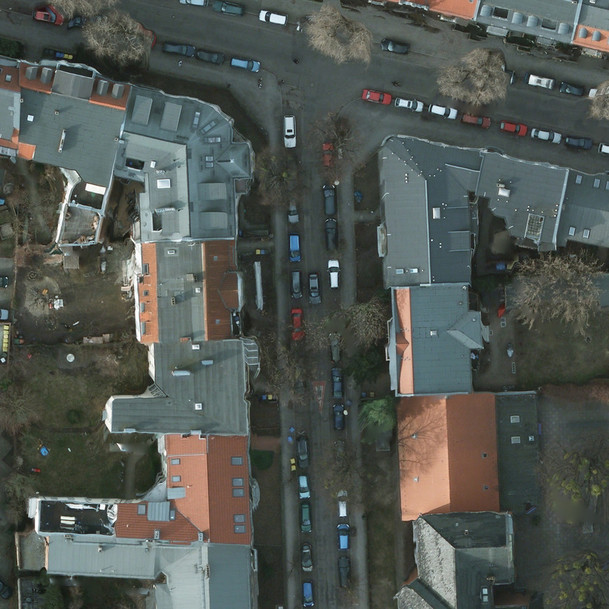
\includegraphics[width=6.3cm]{../Chapitre2/potsdam_sample.jpg}};
     \node [transform shape, rotate=-90, below] at (source.west) {\huge{Optique}};
    \end{scope}

\convlayer{\size}{\size}{\depth}{}{blue}{\segx}{\segy}{\segz}{}
\convlayer{\size}{\size}{\depth}{}{blue}{\segx+\depth}{\segy}{\segz}{}
\convlayer{\size}{\size}{\depth}{}{yellow}{\segx+2*\depth}{\segy}{\segz}{}
\node (add1) at (\segx+3.5*\depth, \segy-0.5*\size, \segz+0.1*\size) {};
\node (pool1) at (\segx+2*\depth, \segy+0.5*\size) {};
\convlayer{\size}{\size}{\depth}{}{cyan}{\segx+3*\depth}{\segy}{\segz}{}

\pgfmathsetmacro\segx{\segx+0.3*\scale}
\pgfmathsetmacro\depth{2*\depth}
\pgfmathsetmacro\size{0.75*\size}

\convlayer{\size}{\size}{\depth}{}{blue}{\segx}{\segy}{\segz}{}
\convlayer{\size}{\size}{\depth}{}{blue}{\segx+\depth}{\segy}{\segz}{}
\convlayer{\size}{\size}{\depth}{}{yellow}{\segx+2*\depth}{\segy}{\segz}{}
\node (add2) at (\segx+3.5*\depth, \segy-0.5*\size, \segz+0.2*\size) {};
\convlayer{\size}{\size}{\depth}{}{cyan}{\segx+3*\depth}{\segy}{\segz}{}
\node (pool2) at (\segx+2*\depth, \segy+0.5*\size) {};

\pgfmathsetmacro\segx{\segx+0.4*\scale}
\pgfmathsetmacro\depth{1.25*\depth}
\pgfmathsetmacro\size{0.75*\size}

\convlayer{\size}{\size}{\depth}{}{blue}{\segx}{\segy}{\segz}{}
\convlayer{\size}{\size}{\depth}{}{blue}{\segx+\depth}{\segy}{\segz}{}
\convlayer{\size}{\size}{\depth}{}{blue}{\segx+2*\depth}{\segy}{\segz}{}
\convlayer{\size}{\size}{\depth}{}{yellow}{\segx+3*\depth}{\segy}{\segz}{}
%\node at (\segx+0.25*\size,\segy-\size) {\huge Encodeur};
\node (add3) at (\segx+4.5*\depth, \segy-0.5*\size, \segz+0.3*\size) {};
\node (pool3) at (\segx+3*\depth, \segy+0.5*\size) {};
\convlayer{\size}{\size}{\depth}{}{cyan}{\segx+4*\depth}{\segy}{\segz}{}

\pgfmathsetmacro\segx{\segx+0.5*\scale}
\pgfmathsetmacro\depth{1.25*\depth}
\pgfmathsetmacro\size{0.75*\size}

\convlayer{\size}{\size}{\depth}{}{blue}{\segx}{\segy}{\segz}{}
\convlayer{\size}{\size}{\depth}{}{blue}{\segx+\depth}{\segy}{\segz}{}
\convlayer{\size}{\size}{\depth}{}{blue}{\segx+2*\depth}{\segy}{\segz}{}
\convlayer{\size}{\size}{\depth}{}{yellow}{\segx+3*\depth}{\segy}{\segz}{}
\node (add4) at (\segx+4*\depth, \segy-0.5*\size, \segz+0.5*\size) {};
\node (pool4) at (\segx+3*\depth, \segy+0.5*\size) {};
\convlayer{\size}{\size}{\depth}{}{cyan}{\segx+4*\depth}{\segy}{\segz}{}

\pgfmathsetmacro\segx{\segx+0.6*\scale}
\pgfmathsetmacro\depth{1.25*\depth}
\pgfmathsetmacro\size{0.75*\size}

\convlayer{\size}{\size}{\depth}{}{blue}{\segx}{\segy}{\segz}{}
\convlayer{\size}{\size}{\depth}{}{blue}{\segx+\depth}{\segy}{\segz}{}
\convlayer{\size}{\size}{\depth}{}{blue}{\segx+2*\depth}{\segy}{\segz}{}
\convlayer{\size}{\size}{\depth}{}{yellow}{\segx+3*\depth}{\segy}{\segz}{}
\node (add5) at (\segx+4*\depth, \segy-0.5*\size, \segz+0.5*\size) {};
\node (pool5) at (\segx+3*\depth, \segy+0.5*\size) {};
\convlayer{\size}{\size}{\depth}{}{cyan}{\segx+4*\depth}{\segy}{\segz}{}

\def\segx{0}
\def\segy{-0.8*\scale}
\def\segz{0}
\def\depth{0.03*\scale}
\def\size{\scale}
%%% ENCODEUR COMP
    \begin{scope}[canvas is yz plane at x=-\segx-0.4*\scale]
     \node[transform shape] (source) at (\segy, 0) {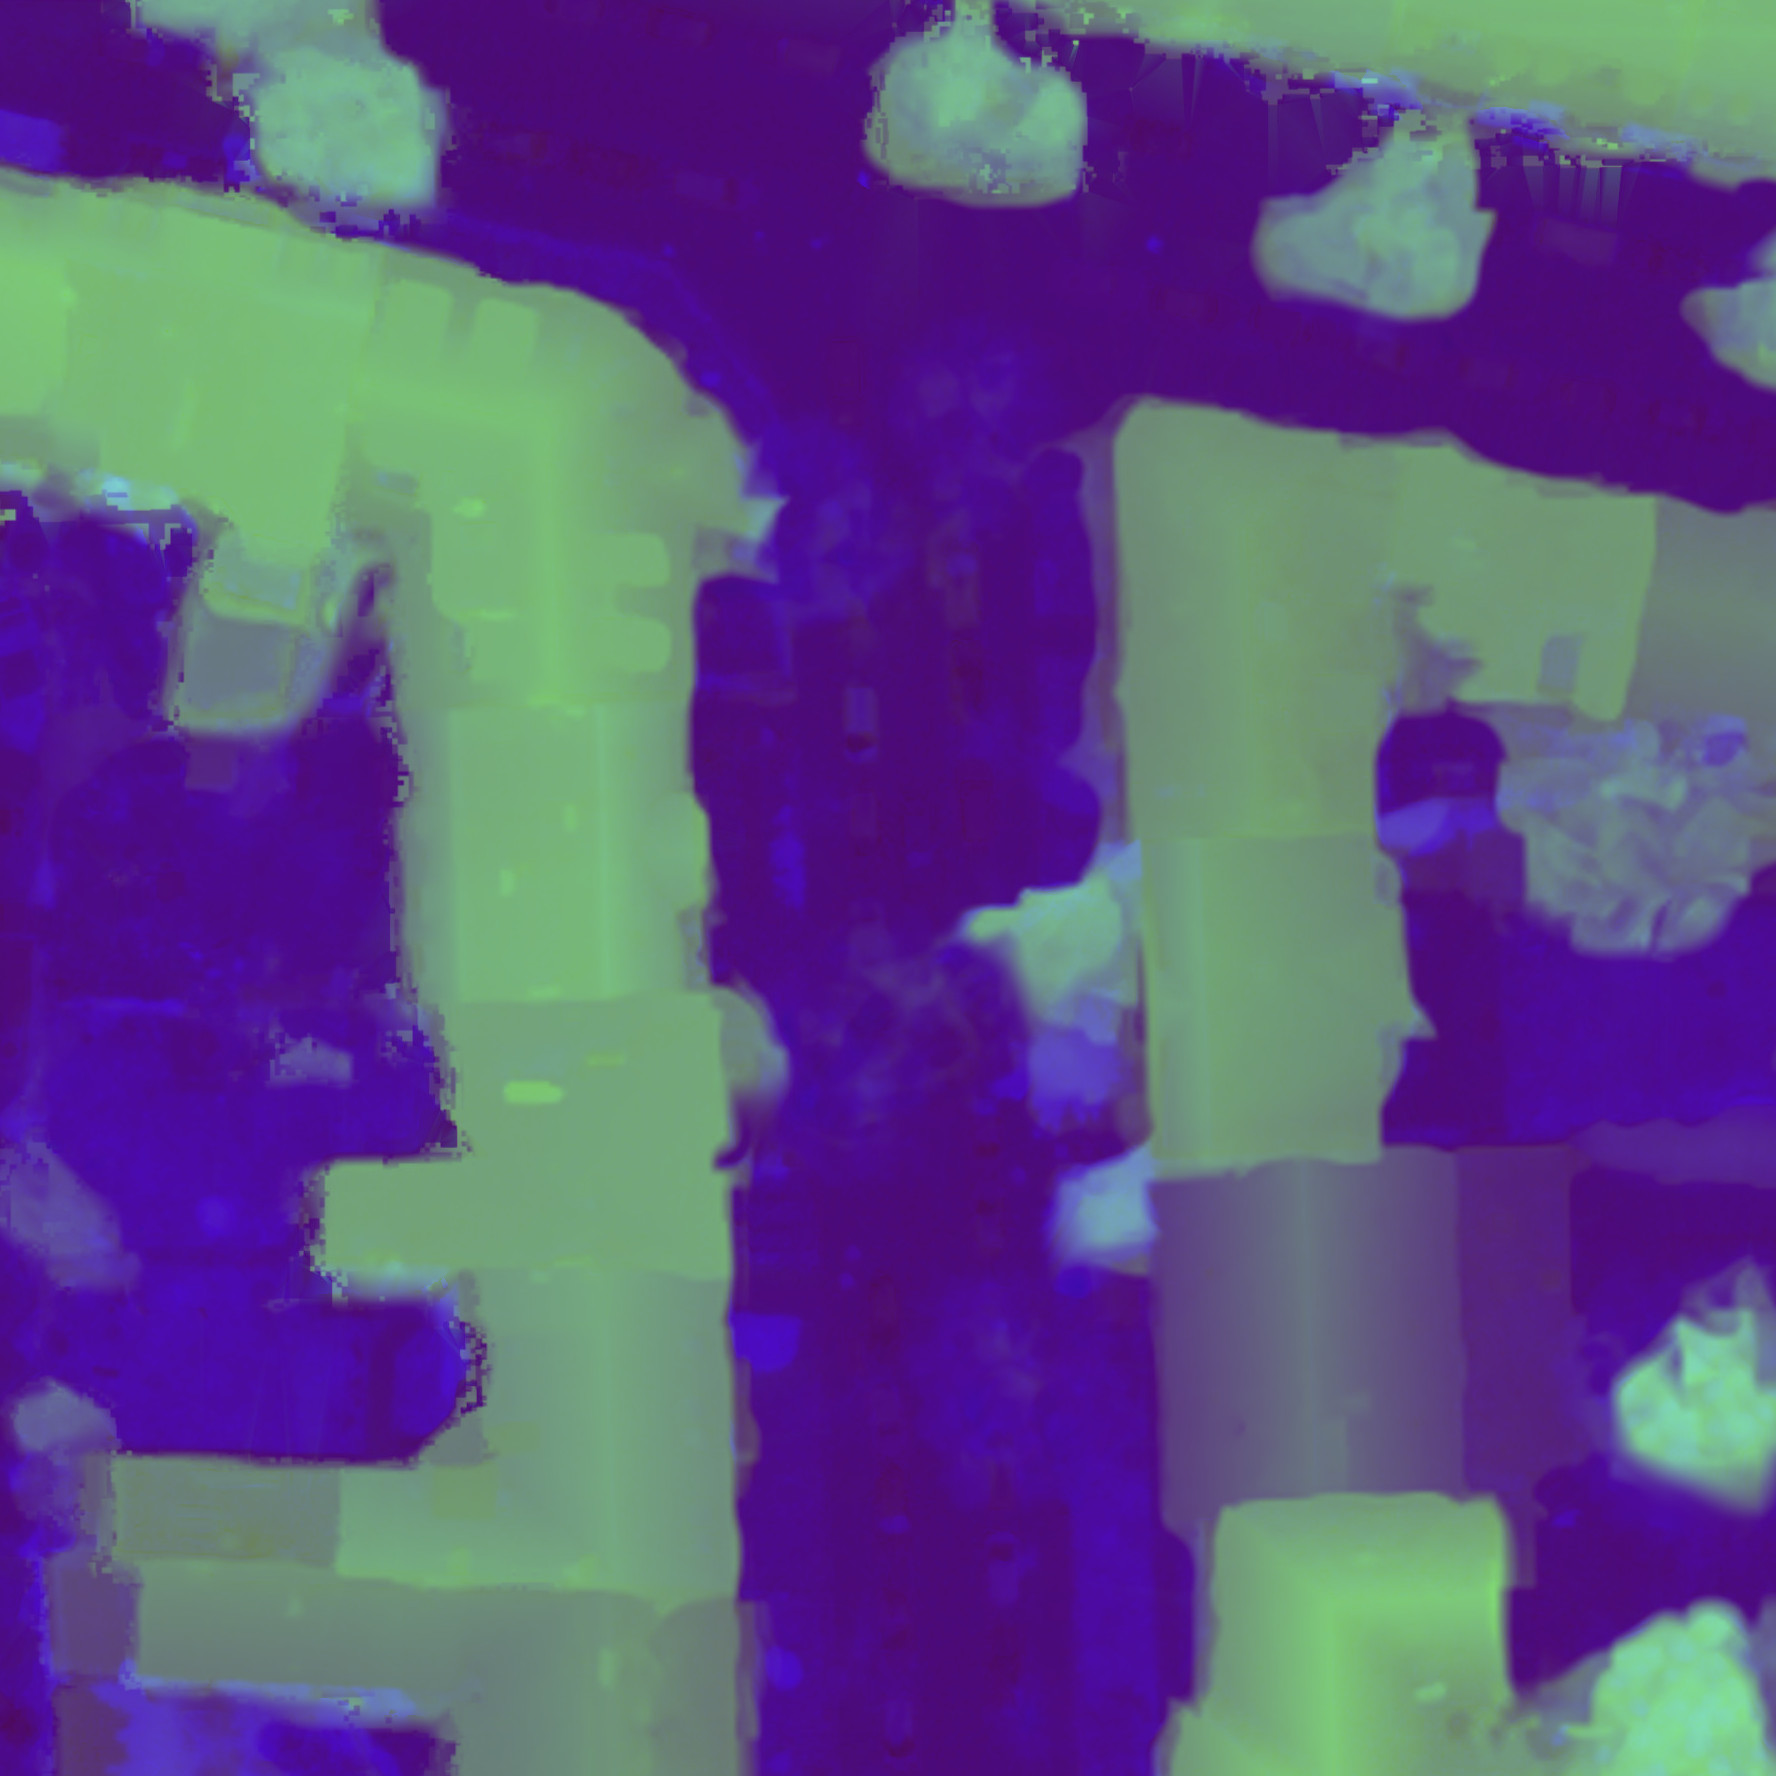
\includegraphics[width=6.3cm]{../Chapitre2/potsdam_sample_composite.jpg}};
     \node [transform shape, rotate=-90, below] at (source.west) {\huge{Composite}};
    \end{scope}

\convlayer{\size}{\size}{\depth}{}{blue}{\segx}{\segy}{\segz}{}
\convlayer{\size}{\size}{\depth}{}{blue}{\segx+\depth}{\segy}{\segz}{}
\convlayer{\size}{\size}{\depth}{}{yellow}{\segx+2*\depth}{\segy}{\segz}{}
\node (cpool1) at (\segx+2*\depth, \segy+0.5*\size) {};

\pgfmathsetmacro\segx{\segx+0.3*\scale}
\pgfmathsetmacro\depth{2*\depth}
\pgfmathsetmacro\size{0.75*\size}

\convlayer{\size}{\size}{\depth}{}{blue}{\segx}{\segy}{\segz}{}
\convlayer{\size}{\size}{\depth}{}{blue}{\segx+\depth}{\segy}{\segz}{}
\convlayer{\size}{\size}{\depth}{}{yellow}{\segx+2*\depth}{\segy}{\segz}{}
\node (cpool2) at (\segx+2*\depth, \segy+0.5*\size) {};

\pgfmathsetmacro\segx{\segx+0.4*\scale}
\pgfmathsetmacro\depth{1.25*\depth}
\pgfmathsetmacro\size{0.75*\size}

\convlayer{\size}{\size}{\depth}{}{blue}{\segx}{\segy}{\segz}{}
\convlayer{\size}{\size}{\depth}{}{blue}{\segx+\depth}{\segy}{\segz}{}
\convlayer{\size}{\size}{\depth}{}{blue}{\segx+2*\depth}{\segy}{\segz}{}
\convlayer{\size}{\size}{\depth}{}{yellow}{\segx+3*\depth}{\segy}{\segz}{}
\node at (\segx+0.25*\size,\segy-\size) {\huge Encodeurs};
\node (cpool3) at (\segx+3*\depth, \segy+0.5*\size) {};

\pgfmathsetmacro\segx{\segx+0.5*\scale}
\pgfmathsetmacro\depth{1.25*\depth}
\pgfmathsetmacro\size{0.75*\size}

\convlayer{\size}{\size}{\depth}{}{blue}{\segx}{\segy}{\segz}{}
\convlayer{\size}{\size}{\depth}{}{blue}{\segx+\depth}{\segy}{\segz}{}
\convlayer{\size}{\size}{\depth}{}{blue}{\segx+2*\depth}{\segy}{\segz}{}
\convlayer{\size}{\size}{\depth}{}{yellow}{\segx+3*\depth}{\segy}{\segz}{}
\node (cpool4) at (\segx+3*\depth, \segy+0.5*\size) {};

\pgfmathsetmacro\segx{\segx+0.6*\scale}
\pgfmathsetmacro\depth{1.25*\depth}
\pgfmathsetmacro\size{0.75*\size}

\convlayer{\size}{\size}{\depth}{}{blue}{\segx}{\segy}{\segz}{}
\convlayer{\size}{\size}{\depth}{}{blue}{\segx+\depth}{\segy}{\segz}{}
\convlayer{\size}{\size}{\depth}{}{blue}{\segx+2*\depth}{\segy}{\segz}{}
\convlayer{\size}{\size}{\depth}{}{yellow}{\segx+3*\depth}{\segy}{\segz}{}
\node (cpool5) at (\segx+3*\depth, \segy+0.5*\size) {};


%%%%% DECODER %%%%%%%%
\pgfmathsetmacro\segx{\segx+0.65*\scale}
\def\segy{+0.8*\scale}

\node (unpool5) at (\segx+0.5*\depth, \segy+0.5*\size) {};
\convlayer{\size}{\size}{\depth}{}{red}{\segx}{\segy}{\segz}{}
\convlayer{\size}{\size}{\depth}{}{blue}{\segx+\depth}{\segy}{\segz}{}
\convlayer{\size}{\size}{\depth}{}{blue}{\segx+2*\depth}{\segy}{\segz}{}
\convlayer{\size}{\size}{\depth}{}{blue}{\segx+3*\depth}{\segy}{\segz}{}

\pgfmathsetmacro\segx{\segx+0.6*\scale}
\pgfmathsetmacro\depth{0.8*\depth}
\pgfmathsetmacro\size{1.33*\size}

\node (unpool4) at (\segx+0.5*\depth, \segy+0.5*\size) {};
\convlayer{\size}{\size}{\depth}{}{red}{\segx}{\segy}{\segz}{}
\convlayer{\size}{\size}{\depth}{}{blue}{\segx+\depth}{\segy}{\segz}{}
\convlayer{\size}{\size}{\depth}{}{blue}{\segx+2*\depth}{\segy}{\segz}{}
\convlayer{\size}{\size}{\depth}{}{blue}{\segx+3*\depth}{\segy}{\segz}{}

\pgfmathsetmacro\segx{\segx+0.5*\scale}
\pgfmathsetmacro\depth{0.8*\depth}
\pgfmathsetmacro\size{1.33*\size}

\node (unpool3) at (\segx+0.5*\depth, \segy+0.5*\size) {};
\convlayer{\size}{\size}{\depth}{}{red}{\segx}{\segy}{\segz}{}
\convlayer{\size}{\size}{\depth}{}{blue}{\segx+\depth}{\segy}{\segz}{}
\convlayer{\size}{\size}{\depth}{}{blue}{\segx+2*\depth}{\segy}{\segz}{}
\convlayer{\size}{\size}{\depth}{}{blue}{\segx+3*\depth}{\segy}{\segz}{}
\node at (\segx-0.25*\size,\segy-\size) {\huge Décodeur};

\pgfmathsetmacro\segx{\segx+0.4*\scale}
\pgfmathsetmacro\depth{0.8*\depth}
\pgfmathsetmacro\size{1.33*\size}

\node (unpool2) at (\segx+0.5*\depth, \segy+0.5*\size) {};
\convlayer{\size}{\size}{\depth}{}{red}{\segx}{\segy}{\segz}{}
\convlayer{\size}{\size}{\depth}{}{blue}{\segx+\depth}{\segy}{\segz}{}
\convlayer{\size}{\size}{\depth}{}{blue}{\segx+2*\depth}{\segy}{\segz}{}

\pgfmathsetmacro\segx{\segx+0.3*\scale}
\pgfmathsetmacro\depth{0.8*\depth}
\pgfmathsetmacro\size{1.33*\size}

\node (unpool1) at (\segx+0.5*\depth, \segy+0.5*\size) {};
\convlayer{\size}{\size}{\depth}{}{red}{\segx}{\segy}{\segz}{}
\convlayer{\size}{\size}{\depth}{}{blue}{\segx+\depth}{\segy}{\segz}{}
\convlayer{\size}{\size}{\depth}{}{blue}{\segx+2*\depth}{\segy}{\segz}{}

\pgfmathsetmacro\segx{\segx+0.3*\scale}
\convlayer{\size}{\size}{0.15\scale}{Prédictions}{brown}{\segx}{\segy}{\segz}{}

\pgfmathsetmacro\segx{\segx+0.3*\scale}
\convlayer{\size}{\size}{0.15\scale}{Softmax}{green}{\segx}{\segy}{\segz}{}

\pgfmathsetmacro\segx{\segx+0.35*\scale}
    \begin{scope}[canvas is yz plane at x=\segx]
     \node[transform shape] (output) at (\segy, 0) {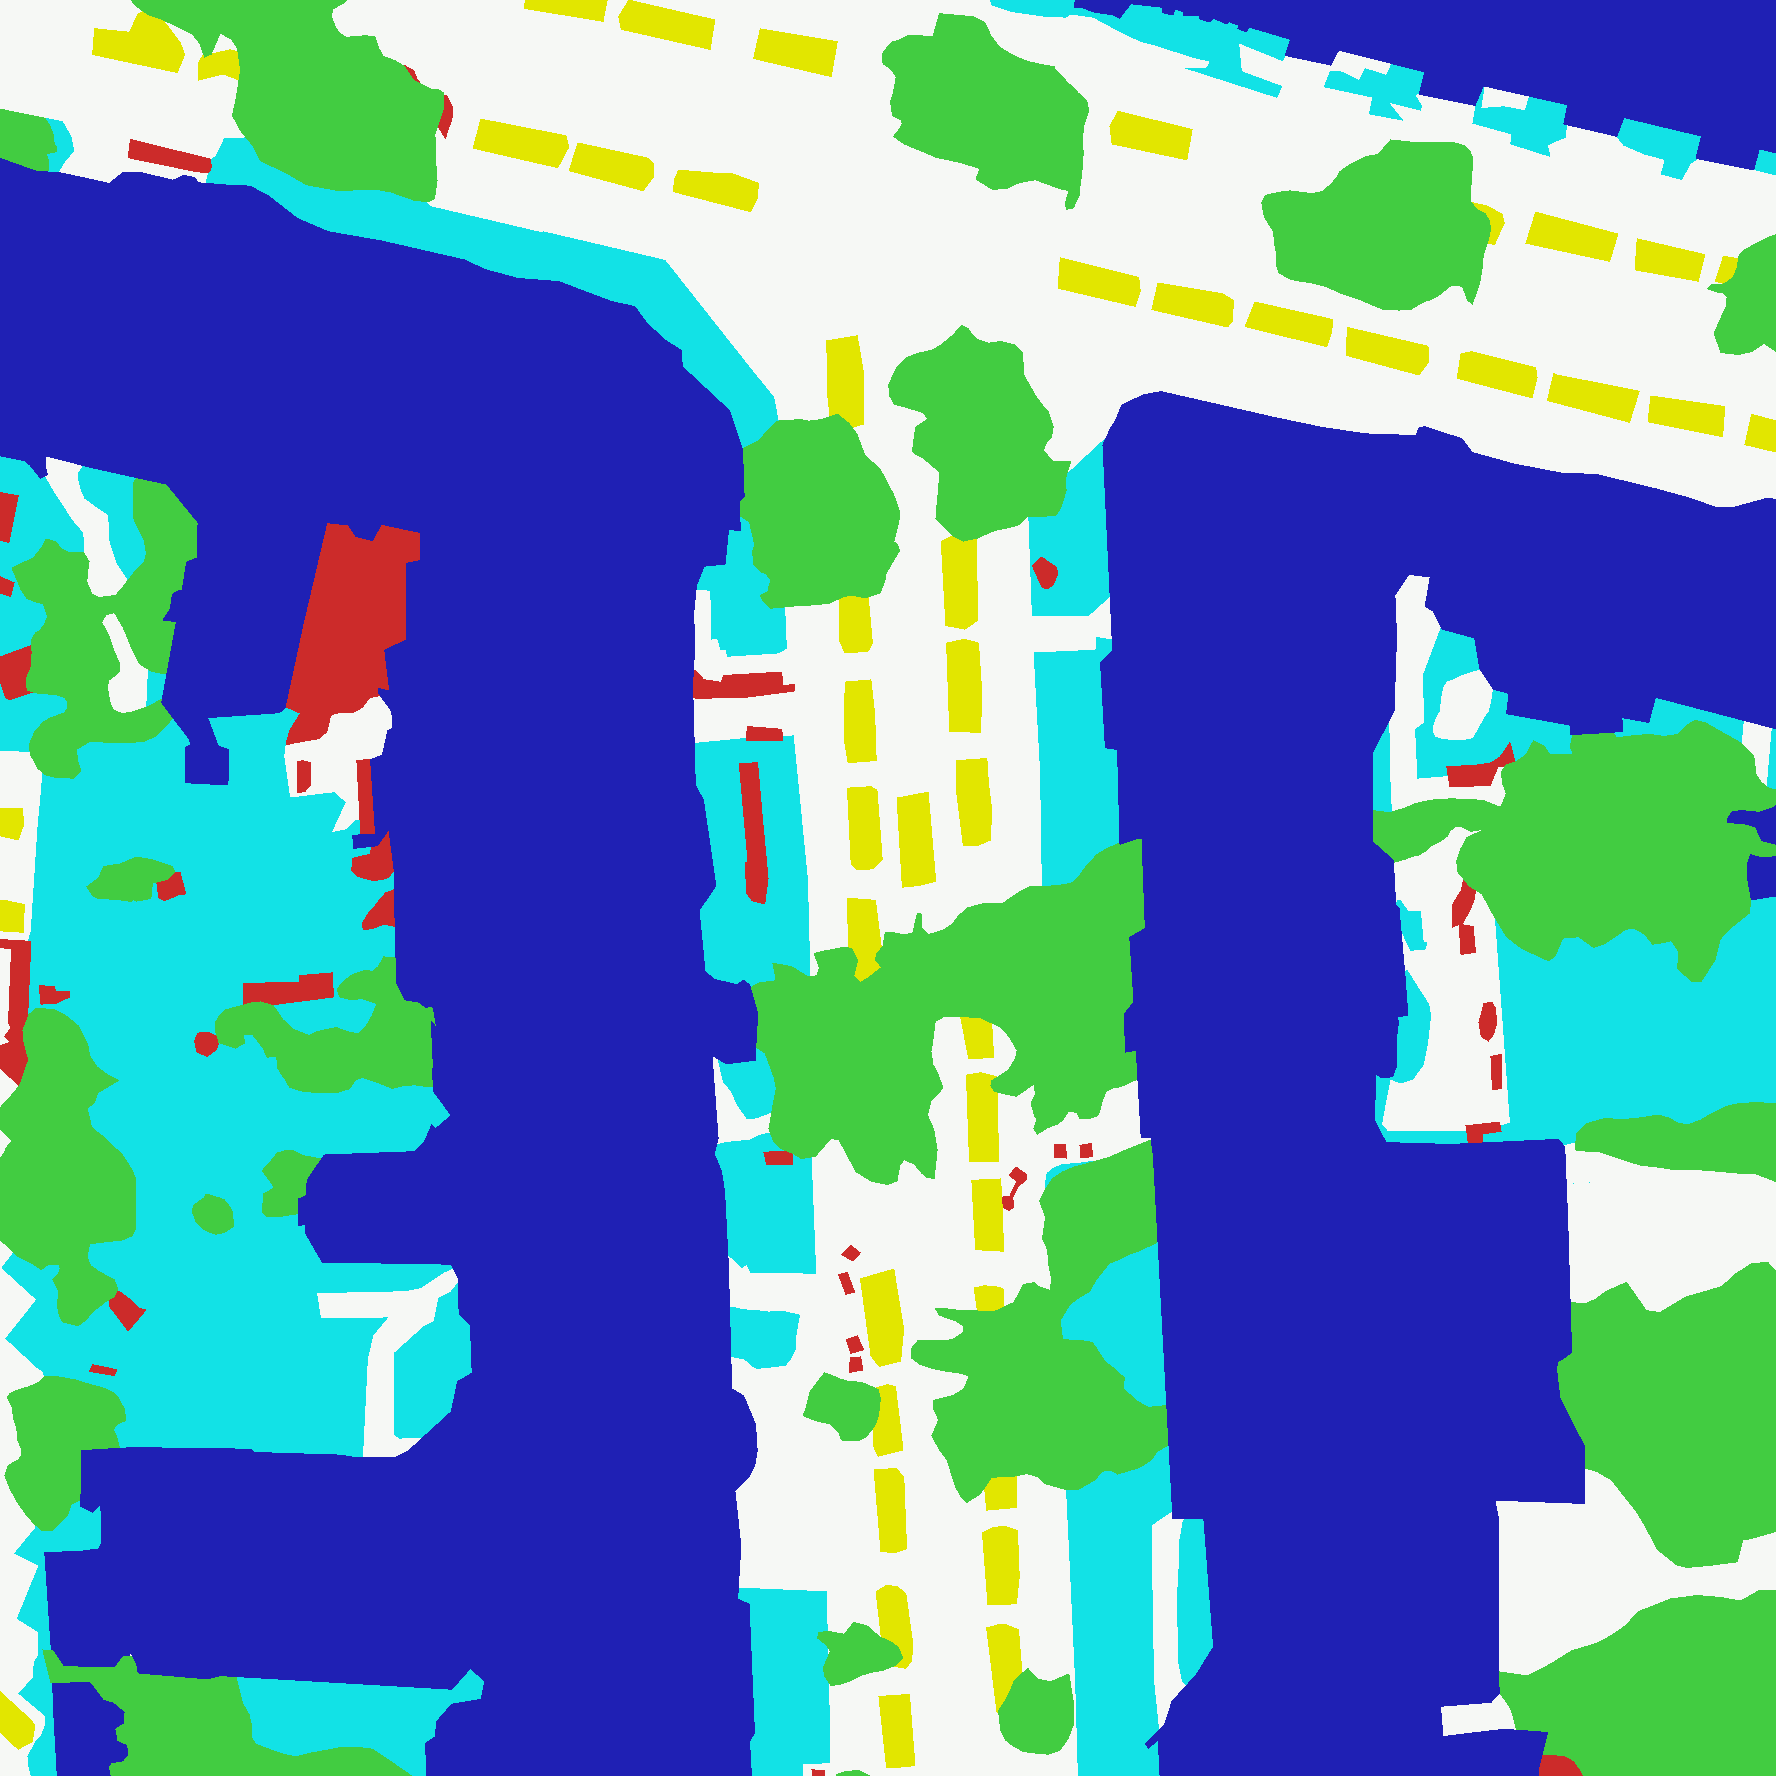
\includegraphics[width=5.5cm]{../Chapitre2/potsdam_sample_gt}};
    \node [transform shape, rotate=-90, below] at (output.west) {\huge{Segmentation}};
    \end{scope}

\tikzset{
    shadowed/.style={preaction={draw opacity=0.75,transform canvas={shift={(1pt,-1pt)}},draw=gray,very thick,dash pattern=on 12pt off 6pt}},
  }

\newcommand\fuseconnection[3][]{%{node1}{node2}
    \draw[shadowed,->,draw opacity=0.75,draw=blue!70!black,ultra thick, dash pattern=on 12pt off 6pt] (#2.center) to[in=-70,out=110] node[xshift=-0.2cm,above, rotate=75,opacity=0.75] {\color{blue!70!black} \Large \textbf{#1}} node[rotate=-12] {\color{blue!70!black} \Huge $$} (#3.center);
}
\fuseconnection{cpool1}{add1}
\fuseconnection{cpool2}{add2}
\fuseconnection{cpool3}{add3}
\fuseconnection{cpool4}{add4}
\fuseconnection[somme]{cpool5}{add5}

\newcommand\skipconnection[3][]{%{node1}{node2}
    \draw[->, very thick,opacity=0.8,dotted,thick] (#2) -- ++(0.085*\size, 0.1*\scale) -- node[above] {#1} ($(#3)+(-0.085*\size, 0.1*\scale)$) -- (#3);
}
\skipconnection{pool5}{unpool5}
\skipconnection{pool4}{unpool4}
\skipconnection{pool3}{unpool3}
\skipconnection{pool2}{unpool2}
\skipconnection[indices]{pool1}{unpool1}

\newcommand\legendlayer[4]{%{name}{x}{color}{y}
\convlayer{0.1*\scale}{0.1*\scale}{0.2*\scale}{}{#3}{#2}{#4}{0}{}
\node[anchor=west] at (#2+0.125*\scale, #4) {\large = #1};
}
\legendlayer{convolution + BN + ReLU}{2.75*\scale}{blue}{-0.7*\scale}
\legendlayer{\emph{maxpooling}}{4.25*\scale}{yellow}{-0.7*\scale}
\legendlayer{\emph{unpooling}}{2.75*\scale}{red}{-1.2*\scale}
\legendlayer{fusion (addition)}{4.25*\scale}{cyan}{-1.2*\scale}

\end{tikzpicture}


\end{document}
}
    \caption[Architecture FuseNet.]{Architecture FuseNet~\cite{hazirbas_fusenet_2016}.}
    \label{fig:fusenet}
\end{figure}

\section{Fusion de modèles}

\subsection{Fusion par apprentissage}

L'architecture FuseNet~\cite{hazirbas_fusenet_2016} est une variante multi-modale de SegNet. Comme illustré dans la~\cref{fig:fusenet}, FuseNet encode conjointement l'image \gls{RVB} et la carte de profondeur en utilisant deux encodeurs dont les contributions respectives sont additionnées après chaque bloc convolutif. Un décodeur unique réalise alors la reconstruction de la résolution et la classification. Cette approche peut être adaptée à n'importe quel autre \gls{CNN} de base, comme les ResNet.

Dans notre cas, nous pouvons altérer FuseNet de la même façon que nous avons altéré SegNet dans les chapitres précédents, afin de traiter des images de télédétection. En effet, une carte d'élévation comme le \gls{MNE} peut être considérée comme une carte de profondeur associée à une image \gls{RVB}. De fait, nous proposons ainsi d'adapter FuseNet au traitemement d'images de télédétection multi-modales. En pratique, nous utiliserons comme sources d'entrées les images optiques, \gls{RVB} ou \gls{IRRV}, et les images composites générées dans la~\cref{sec:composite}.

\begin{figure}[h]
	\begin{subfigure}{0.48\textwidth}
    	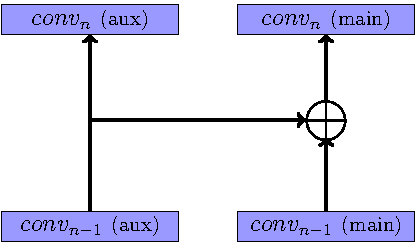
\includegraphics[width=\textwidth]{fusenet_sum.pdf}
        \caption{FuseNet original\,: les activations auxiliaires sont sommées dans la branche principale.}
        \label{fig:fusenet_sum}
    \end{subfigure}
    \hfill
    \begin{subfigure}{0.48\textwidth}
    	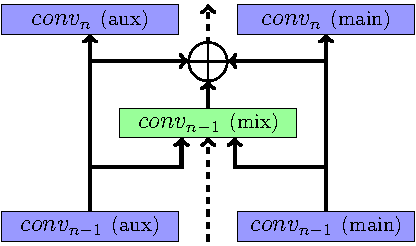
\includegraphics[width=\textwidth]{residual_fusenet.pdf}
        \caption{V-FuseNet: les activations des deux branches sont fusionnées par un bloc convolutif résiduel.}
        \label{fig:fusenet_mix}
    \end{subfigure}
    \caption{Stratégies de fusion pour l'architecture FuseNet.}
\end{figure}

Néanmoins, l'architecture FuseNet considère les données de profondeur comme secondaires. En effet, les deux branches de l'encodeur ne sont pas complètement symétriques\,: la branche de profondeur ne considère que l'information de profondeur tandis que la branche optique opère en réalité sur une représentation conjointe \gls{RGB-D}. De plus, le processus de sur-échantillonnage du décodeur ne considère que les indices de la branche principale, c'est-à-dire la branche optique. Il est donc nécessaire de choisir une source principale de données et une source auxiliaire (cf.~\cref{fig:fusenet_sum}). Il y a donc un déséquilibre fondamental entre les traitements appliqués aux deux sources. Nous proposons une architecture alternative utilisant une troisième source de données virtuelle qui permet de faire disparaître cette asymétrie.

Plutôt que de calculer la somme des cartes d'activations, nous utilisons un processus de fusion permettant d'encoder des caractérstiques multi-modales. Nous introduisons un troisième encodeur qui ne correspond à aucune modalité réelle, mais traite la représentation conjointe des données. Après le $n$\ieme bloc, l'encodeur virtuel concatène les activations des deux encodeurs réels et les transmet à un bloc convolutif résiduel, qui en génère une représentation multi-modale conjointe. Ce sont ces caractéristiques qui sont ensuite décodées et sur-échantillonnées par la deuxième partie du modèle. Ce procédé est illustré par la~\cref{fig:fusenet_mix}. Cette stratégie permet de symétriser FuseNet et de ne plus avoir à choisir de source principale. Cette architecture est nommée \textbf{V-FuseNet} dans le reste du chapitre.

Un autre inconvénient de FuseNet est que cette approche nécessite d'avoir des modèles de base topologiquement compatible afin de pouvoir sommer les activations et fusionner les encodeurs. Cependant, cela ne se vérifie pas systématiquement. Par exemple, certaines données peuvent posséder des natures différentes, comme une image 2D et un nuage de point 3D. En outre, il n'est pas nécessairement utile de consacrer autant de paramètres sur les deux sources de données, notamment si l'une est moins informative que l'autre. Nous proposons donc une méthode de fusion de données alternative pour extraire de l'information à partir de sources hétérogènes. En l'occurrence, nous suggérons d'étudier la possibilité d'effectuer une fusion tardive au moment de la prise de décision, plutôt que d'apprendre des représentations conjointes.

\subsection{Mélanges de modèles}

\begin{figure}[h]
    \resizebox{\textwidth}{!}{\documentclass{standalone}
\usepackage{tikz}
\usepackage{ifthen}
%%%%%%%%%%%%%%%%%%%%%%%%%%%%%%%%%%%%%%%%
%           Commandes perso            %
%%%%%%%%%%%%%%%%%%%%%%%%%%%%%%%%%%%%%%%%

%% Figures centrées, et en position 'here, top, bottom or page'
\newenvironment{figureth}{%
		\begin{figure}[htbp]
			\centering
	}{
		\end{figure}
		}


%% Tableaux centrés, et en position 'here, top, bottom or page'
\newenvironment{tableth}{%
		\begin{table}[htbp]
			\centering
			%\rowcolors{1}{coleurtableau}{coleurtableau}
	}{
		\end{table}
		}

%% Sous-figures centrées, en position 'top'
\newenvironment{subfigureth}[1]{%
	\begin{subfigure}[t]{#1}
	\centering
}{
	\end{subfigure}
}

\newcommand{\citationChap}[2]{%
	\epigraph{\og \textit{#1} \fg{}}{#2}
}

%% On commence par une page impaire quand on change le style de numérotation de pages
\let\oldpagenumbering\pagenumbering
\renewcommand{\pagenumbering}[1]{%
	\cleardoublepage
	\oldpagenumbering{#1}
}

%% Légende du dataset ISPRS
\newcommand\isprslegende{
Légende\,: \textcolor{Black}{blanc}\,: routes, \textcolor{Blue}{bleu}\,: bâtiments, \textcolor{Cerulean}{cyan}\,: végétation basse, \textcolor{OliveGreen}{vert}\,: arbres, \textcolor{Dandelion}{jaune}\,: véhicules, \textcolor{BrickRed}{rouge}\,: autre.
}

%% Dessiner des réseaux de neurones avec Tikz
\newcommand{\convlayer}[9]{%{h}{w}{d}{name}{color}{x}{y}{z}%{note w}{note h}{note d}
   \def\h{#1}
   \def\w{#2}
   \def\d{#3}
   \def\name{#4}
   \ifthenelse {\equal{#5} {}} {\def\col{white}} {\def\col{#5}}
   \def\x{#6}
   \ifthenelse {\equal{#7} {}} {\def\y{0}} {\def\y{#7}}
   \ifthenelse {\equal{#8} {}} {\def\z{0}} {\def\z{#8}}
   % ne faites pas ça chez vous !
   \ifthenelse {\equal{#9} {}} {\convlayercontinued{}{}{}} {\convlayercontinued#9}
}

\newcommand\convlayercontinued[3]{
   \def\notew{#1}
   \def\noteh{#2}
   \def\noted{#3}
   \coordinate (A) at (\x-\d/2,  \y-\h/2, \z-\w/2);
   \coordinate (B) at (\x-\d/2,  \y-\h/2, \z+\w/2);
   \coordinate (C) at (\x-\d/2,  \y+\h/2, \z+\w/2);
   \coordinate (D) at (\x-\d/2,  \y+\h/2, \z-\w/2);
   \coordinate (E) at (\x+\d/2,  \y-\h/2, \z-\w/2);
   \coordinate (F) at (\x+\d/2,  \y-\h/2, \z+\w/2);
   \coordinate (G) at (\x+\d/2,  \y+\h/2, \z+\w/2);
   \coordinate (H) at (\x+\d/2,  \y+\h/2, \z-\w/2);

    \draw [draw opacity=0.3, fill opacity=0.8, fill=\col!60!white] (A) -- (B) -- (C) -- (D) -- cycle;
    \draw [draw opacity=0.3, fill opacity=0.8, fill=\col!60!white] (A) -- (B) -- (F) -- (E) -- cycle;
    % Face haut
    %\draw [left color=\col!60!white, right color=\col!80!white, shading=axis, shading angle=180] (C) -- (D)  -- (H) -- (G) -- cycle;
    \draw [fill opacity=0.9, fill=\col!70!white] (C) -- node[rotate=45,above] {\small \name} (D) -- (H) -- (G) -- cycle;
    %\draw [fill opacity=0.9, fill=\col!70!white] (C) -- (D) -- node[above] {\small \name} (H) -- (G) -- cycle;
    % Face droite
    \draw [fill opacity=0.9, fill=\col!60!white] (E) -- node[pos=0.75,rotate=45,below] {\scriptsize \notew} (F) -- (G) --  (H) -- cycle;
    % Face avant
    %\draw [shading=axis, left color=\col!60!white, right color=\col!40!white, shading angle=-45] (B) -- node[above,rotate=90] {\scriptsize \noteh} (C) -- (G) -- (F) -- node[below] {\scriptsize \noted}  cycle;
    \draw [fill opacity=0.9, fill=\col!50!white] (B) -- node[above,rotate=90] {\scriptsize \noteh} (C) -- (G) -- (F) -- node[below] {\scriptsize \noted}  cycle;
}

\newcommand{\fclayer}[8]{%{h}{w}{name}{color}{x}{y}{z}
   \def\h{#1}
   \def\w{#2}
   \def\name{#3}
   \ifthenelse {\equal{#4} {}} {\def\col{white}} {\def\col{#4}}
   \def\x{#5}
   \def\y{#6}
   \def\z{#7}
   \def\note{#8}
   \coordinate (A) at (\x-\w/2,  \y-\h/2, \z);
   \coordinate (B) at (\x+\w/2,  \y-\h/2, \z);
   \coordinate (C) at (\x+\w/2,  \y+\h/2, \z);
   \coordinate (D) at (\x-\w/2,  \y+\h/2, \z);

   \pgfmathparse{4*\w}\let\boxwidth\pgfmathresult
    \draw [fill=\col] (A) -- node[below,text width=\boxwidth cm,align=center] {\scriptsize \note} (B) -- (C) -- (D) -- cycle;

    \node (N) at ($(A)!0.5!(B)+(0,-1,0)$) {\name};
}

\newcommand{\alexnet}[4]{%{scale}{x}{y}{z}
  \def\scale{#1}
  \def\alexx{#2}
  \def\alexy{#3}
  \def\alexz{#4}


  \def\coblue{blue!50!white}
  \def\fcgrey{gray!50!white}

  \convlayer{1.3*\scale}{1.3*\scale}{0.02*\scale}{Image}{\coblue}{\alexx}{\alexy}{\alexz}{{227}{227}{3}}
  \convlayer{1.1*\scale}{1.1*\scale}{0.08*\scale}{Conv1}{\coblue}{\alexx+0.7*\scale}{\alexy}{\alexz}{{55}{55}{96}}
  \convlayer{0.7*\scale}{0.7*\scale}{0.5*\scale}{Conv2}{\coblue}{\alexx+1.5*\scale}{\alexy}{\alexz}{{27}{27}{256}}
  \convlayer{0.5*\scale}{0.5*\scale}{0.8*\scale}{Conv3}{\coblue}{\alexx+2.6*\scale}{\alexy}{\alexz}{{13}{13}{384}}
  \convlayer{0.5*\scale}{0.5*\scale}{0.8*\scale}{Conv4}{\coblue}{\alexx+3.8*\scale}{\alexy}{\alexz}{{13}{13}{384}}
  \convlayer{0.5*\scale}{0.5*\scale}{0.5*\scale}{Conv5}{\coblue}{\alexx+4.8*\scale}{\alexy}{\alexz}{{13}{13}{256}}
  \fclayer{\scale}{0.1*\scale}{FC1}{\fcgrey}{\alexx+5.4*\scale}{\alexy}{\alexz}{4096}
  \fclayer{\scale}{0.1*\scale}{FC2}{\fcgrey}{\alexx+5.7*\scale}{\alexy}{\alexz}{4096}
  \fclayer{\scale}{0.1*\scale}{FC3}{\fcgrey}{\alexx+6.0*\scale}{\alexy}{\alexz}{1000}
}

\newcommand{\imagelayer}[7]{%{width}{x}{y}{z}{path}{text_up}{text_down}
    \pgfmathparse{#1}\let\w\pgfmathresult
    \begin{scope}[canvas is yz plane at x=#2]
     \node[transform shape] (source) at (#3, #4) {\includegraphics[angle=-90,width=\w cm]{#5}};
    \end{scope}
     \node [transform shape, rotate=45, above] at (source.east) {#6};
     \node [transform shape, rotate=45, below] at (source.west) {\scriptsize{#7}};
}

\def\fourier{\mathcal{F}}

\newcommand{\lightspectrum}{%
\pgfplotsset{
    % this *defines* a custom colormap ...
    colormap={slategraywhite}{color(0cm)=(red); color(1cm)=(red); color(2cm)=(red); color(3cm)=(red); color(4cm)=(orange); color(5cm)=(yellow); color(6cm)=(green); color(7cm)=(blue); color(8cm)=(blue); color(9cm)=(purple); color(10cm)=(purple); color(12cm)=(black)}
}
\node at (1.5, 2.7) {\small 1mm};
\node at (4, 3) {Infrarouge};
\node at (7.75, 2.7) {\small 800nm};
\node at (9, 3) {Visible};
\node at (10.5, 2.7) {\small 400nm};
\node at (12, 3) {Ultraviolet};
\node at (13.5, 2.7) {\small 10nm};
\draw[->] (1, 2.5) -- (14, 2.5);
\begin{axis}[hide axis,width=16cm,height=4cm,colormap name=slategraywhite]
\addplot[domain=20:1000,samples=1500,ultra thick, point meta=x*x,mesh]{sin(x*x/80)};
\end{axis}
}

% Union généralisée
\newcommand{\wbigcup}{\mathop{\bigcup}\displaylimits}

\newcommand{\res}[2]{#1 {\footnotesize $\pm$ #2}}
\newcommand{\bres}[2]{\textbf{#1} {\footnotesize $\pm$ #2}}
\newcommand{\bbres}[2]{\res{\textit{#1}}{#2}}

\newcommand{\drawkernel}[9]{
\begin{tikzpicture}
	\draw[step=1cm,gray!50!white,very thin] (0,0) grid (3,3);
	\kernelnode{0.5}{0.5}{#1};
	\kernelnode{0.5}{1.5}{#2};
	\kernelnode{0.5}{2.5}{#3};
	\kernelnode{1.5}{0.5}{#4};
	\kernelnode{1.5}{1.5}{#5};
	\kernelnode{1.5}{2.5}{#6};
	\kernelnode{2.5}{0.5}{#7};
	\kernelnode{2.5}{1.5}{#8};
	\kernelnode{2.5}{2.5}{#9};
\end{tikzpicture}
}

\newcommand{\kernelnode}[3]{%{x}{y}{value}
	\ifthenelse{\equal{#3}{0}}{
		\def\kcolor{gray}
	}{
		\def\kcolor{black}
	}
	\node[\kcolor] at (#1, #2) {#3};
}

\newcommand{\chapsummary}[1]{
\section*{Résumé du chapitre :}
\parbox{0.9\linewidth}{
\setlength{\parindent}{4ex}
#1}
}

\newcommand{\eqname}[1]{\tag*{\small (#1)}}

\begin{document}

\begin{tikzpicture}[]
\usetikzlibrary{3d}
\usetikzlibrary{calc}

\def\scale{5}
\def\segx{0}
\def\segy{+0.8*\scale}
\def\segz{0}
\def\depth{0.03*\scale}
\def\size{\scale}

    \begin{scope}[canvas is yz plane at x=-\segx-0.4*\scale]
     \node[transform shape] (source) at (\segy, 0) {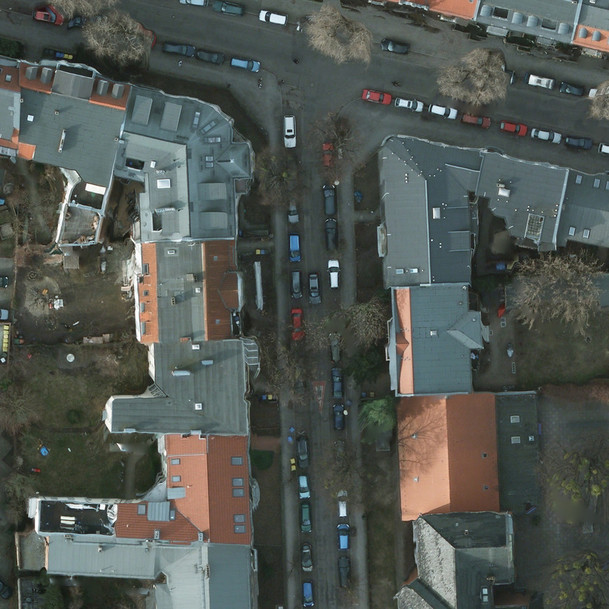
\includegraphics[width=6.3cm]{../Chapitre2/potsdam_sample.jpg}};
     \node [transform shape, rotate=-90, below] at (source.west) {\huge{Optique}};
    \end{scope}

\convlayer{\size}{\size}{\depth}{}{blue}{\segx}{\segy}{\segz}{}
\convlayer{\size}{\size}{\depth}{}{blue}{\segx+\depth}{\segy}{\segz}{}
\convlayer{\size}{\size}{\depth}{}{yellow}{\segx+2*\depth}{\segy}{\segz}{}
\node (pool1) at (\segx+2*\depth, \segy+0.5*\size) {};

\pgfmathsetmacro\segx{\segx+0.3*\scale}
\pgfmathsetmacro\depth{2*\depth}
\pgfmathsetmacro\size{0.75*\size}

\convlayer{\size}{\size}{\depth}{}{blue}{\segx}{\segy}{\segz}{}
\convlayer{\size}{\size}{\depth}{}{blue}{\segx+\depth}{\segy}{\segz}{}
\convlayer{\size}{\size}{\depth}{}{yellow}{\segx+2*\depth}{\segy}{\segz}{}
\node (pool2) at (\segx+2*\depth, \segy+0.5*\size) {};

\pgfmathsetmacro\segx{\segx+0.4*\scale}
\pgfmathsetmacro\depth{1.25*\depth}
\pgfmathsetmacro\size{0.75*\size}

\convlayer{\size}{\size}{\depth}{}{blue}{\segx}{\segy}{\segz}{}
\convlayer{\size}{\size}{\depth}{}{blue}{\segx+\depth}{\segy}{\segz}{}
\convlayer{\size}{\size}{\depth}{}{blue}{\segx+2*\depth}{\segy}{\segz}{}
\convlayer{\size}{\size}{\depth}{}{yellow}{\segx+3*\depth}{\segy}{\segz}{}
\node at (\segx+0.25*\size,\segy-\size) {\huge Encodeur};
\node (pool3) at (\segx+3*\depth, \segy+0.5*\size) {};

\pgfmathsetmacro\segx{\segx+0.5*\scale}
\pgfmathsetmacro\depth{1.25*\depth}
\pgfmathsetmacro\size{0.75*\size}

\convlayer{\size}{\size}{\depth}{}{blue}{\segx}{\segy}{\segz}{}
\convlayer{\size}{\size}{\depth}{}{blue}{\segx+\depth}{\segy}{\segz}{}
\convlayer{\size}{\size}{\depth}{}{blue}{\segx+2*\depth}{\segy}{\segz}{}
\convlayer{\size}{\size}{\depth}{}{yellow}{\segx+3*\depth}{\segy}{\segz}{}
\node (pool4) at (\segx+3*\depth, \segy+0.5*\size) {};

\pgfmathsetmacro\segx{\segx+0.6*\scale}
\pgfmathsetmacro\depth{1.25*\depth}
\pgfmathsetmacro\size{0.75*\size}

\convlayer{\size}{\size}{\depth}{}{blue}{\segx}{\segy}{\segz}{}
\convlayer{\size}{\size}{\depth}{}{blue}{\segx+\depth}{\segy}{\segz}{}
\convlayer{\size}{\size}{\depth}{}{blue}{\segx+2*\depth}{\segy}{\segz}{}
\convlayer{\size}{\size}{\depth}{}{yellow}{\segx+3*\depth}{\segy}{\segz}{}
\node (pool5) at (\segx+3*\depth, \segy+0.5*\size) {};

%%%%% DECODER %%%%%%%%

\pgfmathsetmacro\segx{\segx+0.6*\scale}

\node (unpool5) at (\segx+0.5*\depth, \segy+0.5*\size) {};
\convlayer{\size}{\size}{\depth}{}{red}{\segx}{\segy}{\segz}{}
\convlayer{\size}{\size}{\depth}{}{blue}{\segx+\depth}{\segy}{\segz}{}
\convlayer{\size}{\size}{\depth}{}{blue}{\segx+2*\depth}{\segy}{\segz}{}
\convlayer{\size}{\size}{\depth}{}{blue}{\segx+3*\depth}{\segy}{\segz}{}

\pgfmathsetmacro\segx{\segx+0.6*\scale}
\pgfmathsetmacro\depth{0.8*\depth}
\pgfmathsetmacro\size{1.33*\size}

\node (unpool4) at (\segx+0.5*\depth, \segy+0.5*\size) {};
\convlayer{\size}{\size}{\depth}{}{red}{\segx}{\segy}{\segz}{}
\convlayer{\size}{\size}{\depth}{}{blue}{\segx+\depth}{\segy}{\segz}{}
\convlayer{\size}{\size}{\depth}{}{blue}{\segx+2*\depth}{\segy}{\segz}{}
\convlayer{\size}{\size}{\depth}{}{blue}{\segx+3*\depth}{\segy}{\segz}{}

\pgfmathsetmacro\segx{\segx+0.5*\scale}
\pgfmathsetmacro\depth{0.8*\depth}
\pgfmathsetmacro\size{1.33*\size}

\node (unpool3) at (\segx+0.5*\depth, \segy+0.5*\size) {};
\convlayer{\size}{\size}{\depth}{}{red}{\segx}{\segy}{\segz}{}
\convlayer{\size}{\size}{\depth}{}{blue}{\segx+\depth}{\segy}{\segz}{}
\convlayer{\size}{\size}{\depth}{}{blue}{\segx+2*\depth}{\segy}{\segz}{}
\convlayer{\size}{\size}{\depth}{}{blue}{\segx+3*\depth}{\segy}{\segz}{}
\node at (\segx-0.25*\size,\segy-\size) {\huge Décodeur};

\pgfmathsetmacro\segx{\segx+0.4*\scale}
\pgfmathsetmacro\depth{0.8*\depth}
\pgfmathsetmacro\size{1.33*\size}

\node (unpool2) at (\segx+0.5*\depth, \segy+0.5*\size) {};
\convlayer{\size}{\size}{\depth}{}{red}{\segx}{\segy}{\segz}{}
\convlayer{\size}{\size}{\depth}{}{blue}{\segx+\depth}{\segy}{\segz}{}
\convlayer{\size}{\size}{\depth}{}{blue}{\segx+2*\depth}{\segy}{\segz}{}

\pgfmathsetmacro\segx{\segx+0.3*\scale}
\pgfmathsetmacro\depth{0.8*\depth}
\pgfmathsetmacro\size{1.33*\size}

\node (unpool1) at (\segx+0.5*\depth, \segy+0.5*\size) {};
\node (o_unpool1) at (\segx+0.5*\depth, \segy-0.56*\size) {};
\convlayer{\size}{\size}{\depth}{}{red}{\segx}{\segy}{\segz}{}
\convlayer{\size}{\size}{\depth}{}{blue}{\segx+\depth}{\segy}{\segz}{}
\convlayer{\size}{\size}{\depth}{}{blue}{\segx+2*\depth}{\segy}{\segz}{}

\pgfmathsetmacro\segx{\segx+0.3*\scale}
\convlayer{\size}{\size}{0.15\scale}{Prédictions}{brown}{\segx}{\segy}{\segz}{}
\node (pred_opt) at (\segx,\segy,\segz) {};

\newcommand\skipconnection[3][]{%{node1}{node2}
    \draw[->, dotted, very thick] (#2) -- ++(0.085*\size, 0.1*\scale) -- node[above] {#1} ($(#3)+(-0.085*\size, 0.1*\scale)$) -- (#3);
}
\skipconnection{pool5}{unpool5}
\skipconnection{pool4}{unpool4}
\skipconnection{pool3}{unpool3}
\skipconnection{pool2}{unpool2}
\skipconnection[indices]{pool1}{unpool1}


\def\segx{0}
\def\segy{-0.8*\scale}
\def\segz{0}
\def\depth{0.03*\scale}
\def\size{\scale}

    \begin{scope}[canvas is yz plane at x=-\segx-0.4*\scale]
     \node[transform shape] (source) at (\segy, 0) {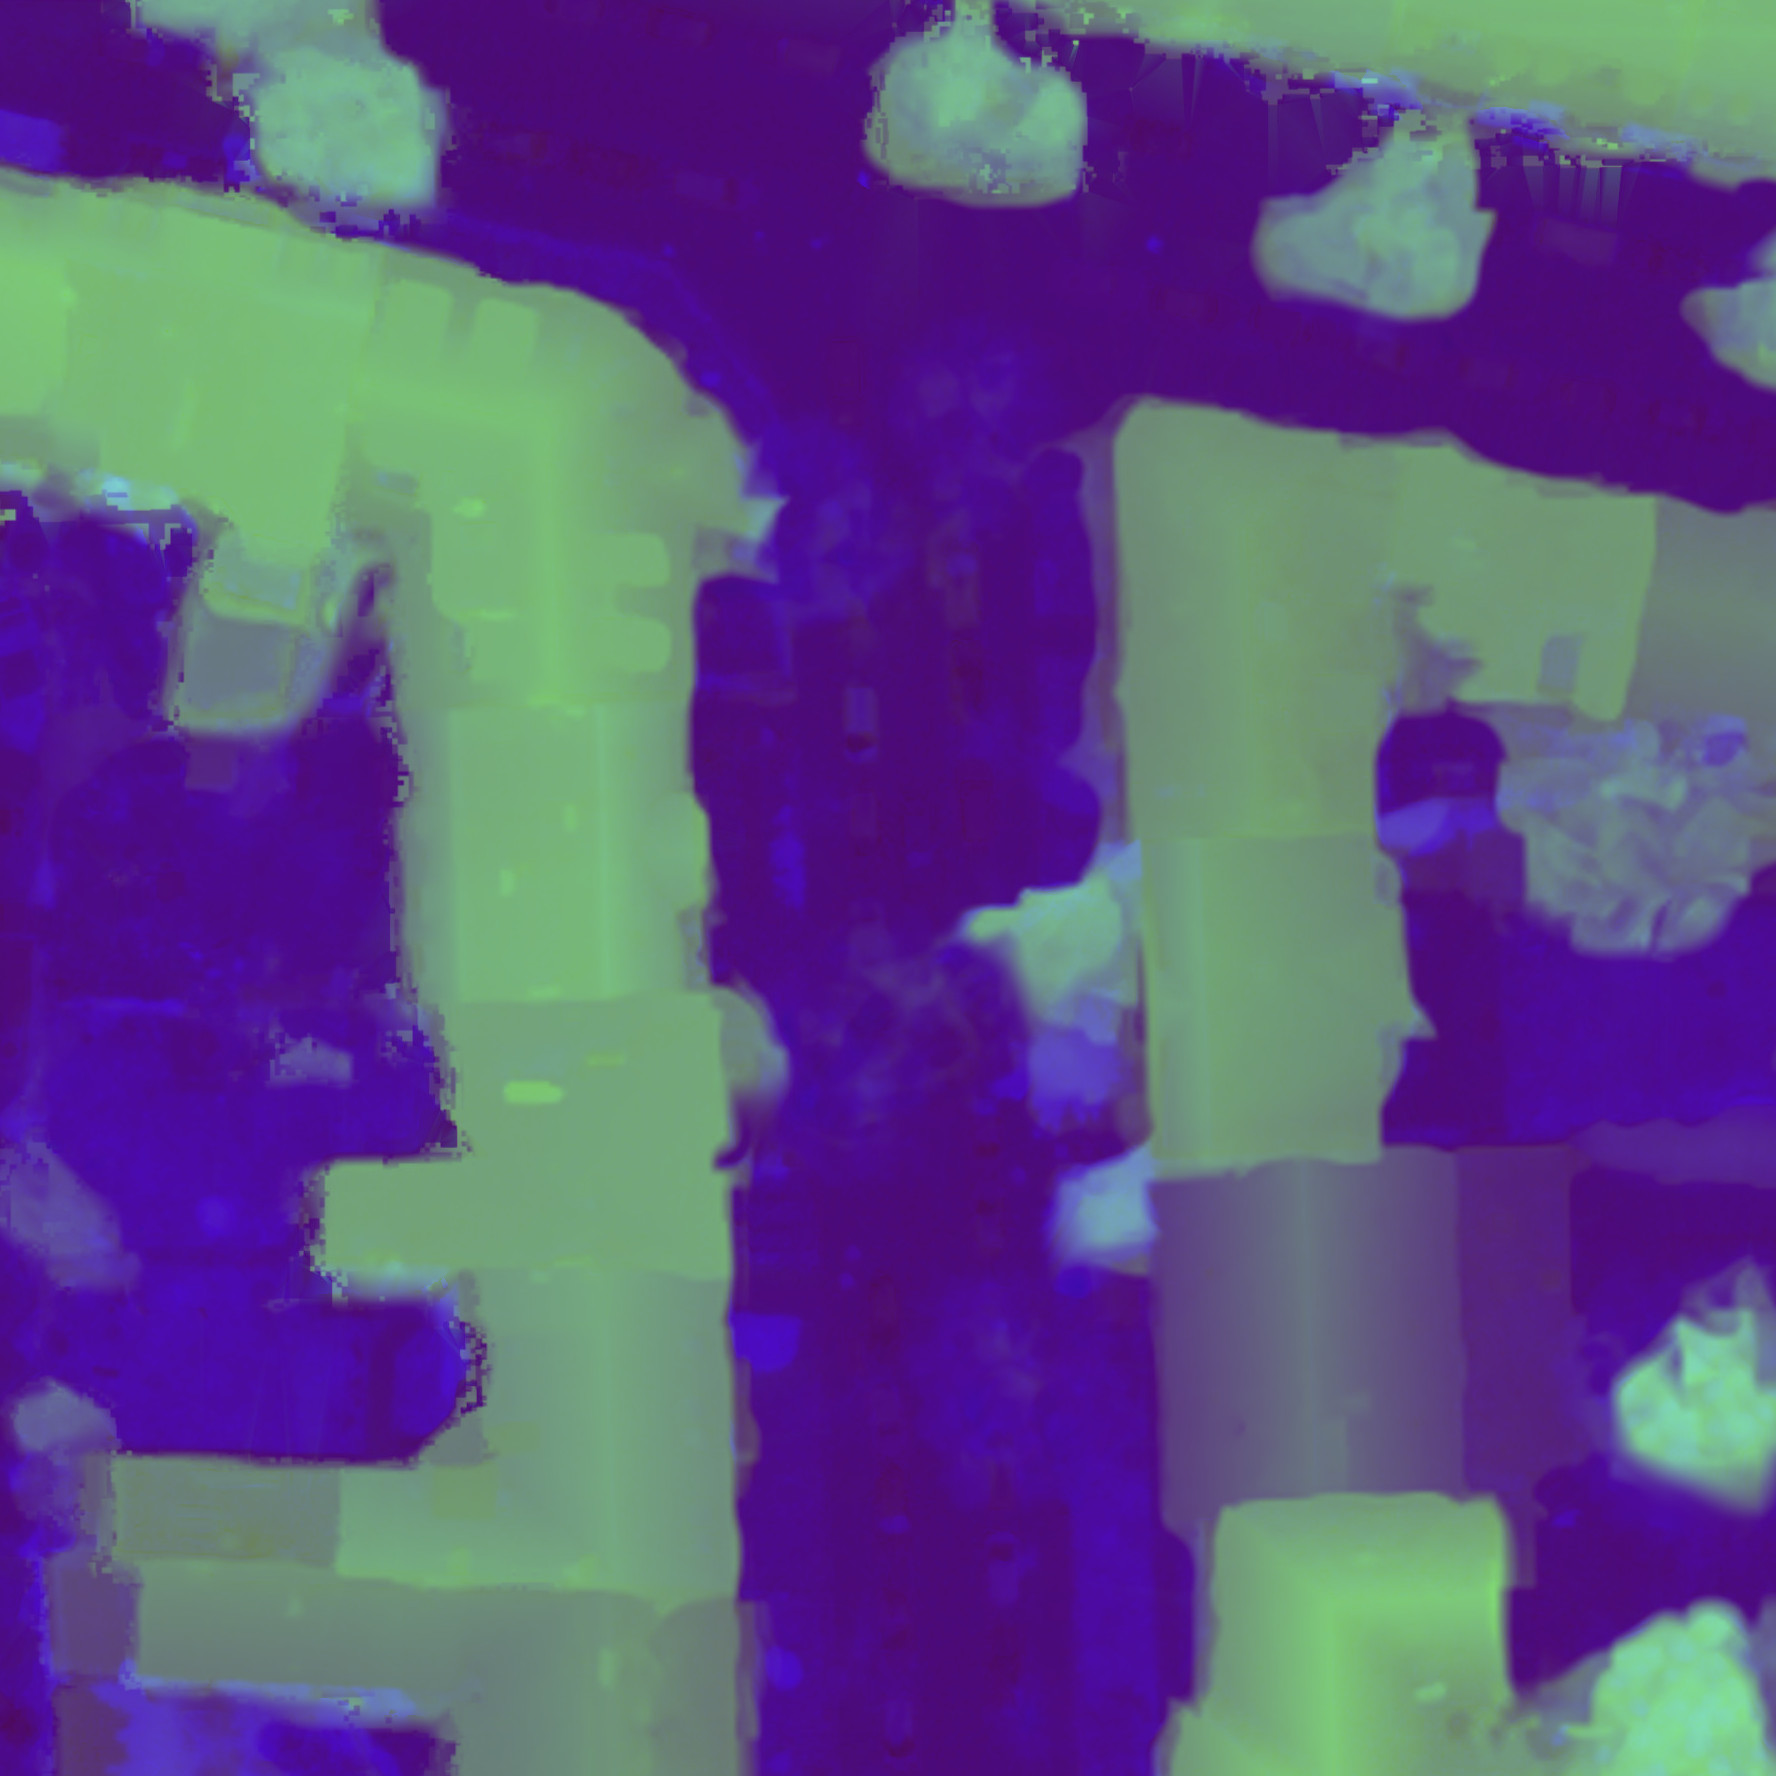
\includegraphics[width=6.3cm]{../Chapitre2/potsdam_sample_composite.jpg}};
     \node [transform shape, rotate=-90, below] at (source.west) {\huge{Composite}};
    \end{scope}

\convlayer{\size}{\size}{\depth}{}{blue}{\segx}{\segy}{\segz}{}
\convlayer{\size}{\size}{\depth}{}{blue}{\segx+\depth}{\segy}{\segz}{}
\convlayer{\size}{\size}{\depth}{}{yellow}{\segx+2*\depth}{\segy}{\segz}{}
\node (pool1) at (\segx+2*\depth, \segy+0.5*\size) {};

\pgfmathsetmacro\segx{\segx+0.3*\scale}
\pgfmathsetmacro\depth{2*\depth}
\pgfmathsetmacro\size{0.75*\size}

\convlayer{\size}{\size}{\depth}{}{blue}{\segx}{\segy}{\segz}{}
\convlayer{\size}{\size}{\depth}{}{blue}{\segx+\depth}{\segy}{\segz}{}
\convlayer{\size}{\size}{\depth}{}{yellow}{\segx+2*\depth}{\segy}{\segz}{}
\node (pool2) at (\segx+2*\depth, \segy+0.5*\size) {};

\pgfmathsetmacro\segx{\segx+0.4*\scale}
\pgfmathsetmacro\depth{1.25*\depth}
\pgfmathsetmacro\size{0.75*\size}

\convlayer{\size}{\size}{\depth}{}{blue}{\segx}{\segy}{\segz}{}
\convlayer{\size}{\size}{\depth}{}{blue}{\segx+\depth}{\segy}{\segz}{}
\convlayer{\size}{\size}{\depth}{}{blue}{\segx+2*\depth}{\segy}{\segz}{}
\convlayer{\size}{\size}{\depth}{}{yellow}{\segx+3*\depth}{\segy}{\segz}{}
\node at (\segx+0.25*\size,\segy-\size) {\huge Encodeur};
\node (pool3) at (\segx+3*\depth, \segy+0.5*\size) {};

\pgfmathsetmacro\segx{\segx+0.5*\scale}
\pgfmathsetmacro\depth{1.25*\depth}
\pgfmathsetmacro\size{0.75*\size}

\convlayer{\size}{\size}{\depth}{}{blue}{\segx}{\segy}{\segz}{}
\convlayer{\size}{\size}{\depth}{}{blue}{\segx+\depth}{\segy}{\segz}{}
\convlayer{\size}{\size}{\depth}{}{blue}{\segx+2*\depth}{\segy}{\segz}{}
\convlayer{\size}{\size}{\depth}{}{yellow}{\segx+3*\depth}{\segy}{\segz}{}
\node (pool4) at (\segx+3*\depth, \segy+0.5*\size) {};

\pgfmathsetmacro\segx{\segx+0.6*\scale}
\pgfmathsetmacro\depth{1.25*\depth}
\pgfmathsetmacro\size{0.75*\size}

\convlayer{\size}{\size}{\depth}{}{blue}{\segx}{\segy}{\segz}{}
\convlayer{\size}{\size}{\depth}{}{blue}{\segx+\depth}{\segy}{\segz}{}
\convlayer{\size}{\size}{\depth}{}{blue}{\segx+2*\depth}{\segy}{\segz}{}
\convlayer{\size}{\size}{\depth}{}{yellow}{\segx+3*\depth}{\segy}{\segz}{}
\node (pool5) at (\segx+3*\depth, \segy+0.5*\size) {};

%%%%% DECODER %%%%%%%%

\pgfmathsetmacro\segx{\segx+0.6*\scale}

\node (unpool5) at (\segx+0.5*\depth, \segy+0.5*\size) {};
\convlayer{\size}{\size}{\depth}{}{red}{\segx}{\segy}{\segz}{}
\convlayer{\size}{\size}{\depth}{}{blue}{\segx+\depth}{\segy}{\segz}{}
\convlayer{\size}{\size}{\depth}{}{blue}{\segx+2*\depth}{\segy}{\segz}{}
\convlayer{\size}{\size}{\depth}{}{blue}{\segx+3*\depth}{\segy}{\segz}{}

\pgfmathsetmacro\segx{\segx+0.6*\scale}
\pgfmathsetmacro\depth{0.8*\depth}
\pgfmathsetmacro\size{1.33*\size}

\node (unpool4) at (\segx+0.5*\depth, \segy+0.5*\size) {};
\convlayer{\size}{\size}{\depth}{}{red}{\segx}{\segy}{\segz}{}
\convlayer{\size}{\size}{\depth}{}{blue}{\segx+\depth}{\segy}{\segz}{}
\convlayer{\size}{\size}{\depth}{}{blue}{\segx+2*\depth}{\segy}{\segz}{}
\convlayer{\size}{\size}{\depth}{}{blue}{\segx+3*\depth}{\segy}{\segz}{}

\pgfmathsetmacro\segx{\segx+0.5*\scale}
\pgfmathsetmacro\depth{0.8*\depth}
\pgfmathsetmacro\size{1.33*\size}

\node (unpool3) at (\segx+0.5*\depth, \segy+0.5*\size) {};
\convlayer{\size}{\size}{\depth}{}{red}{\segx}{\segy}{\segz}{}
\convlayer{\size}{\size}{\depth}{}{blue}{\segx+\depth}{\segy}{\segz}{}
\convlayer{\size}{\size}{\depth}{}{blue}{\segx+2*\depth}{\segy}{\segz}{}
\convlayer{\size}{\size}{\depth}{}{blue}{\segx+3*\depth}{\segy}{\segz}{}
\node at (\segx-0.25*\size,\segy-\size) {\huge Décodeur};

\pgfmathsetmacro\segx{\segx+0.4*\scale}
\pgfmathsetmacro\depth{0.8*\depth}
\pgfmathsetmacro\size{1.33*\size}

\node (unpool2) at (\segx+0.5*\depth, \segy+0.5*\size) {};
\convlayer{\size}{\size}{\depth}{}{red}{\segx}{\segy}{\segz}{}
\convlayer{\size}{\size}{\depth}{}{blue}{\segx+\depth}{\segy}{\segz}{}
\convlayer{\size}{\size}{\depth}{}{blue}{\segx+2*\depth}{\segy}{\segz}{}

\pgfmathsetmacro\segx{\segx+0.3*\scale}
\pgfmathsetmacro\depth{0.8*\depth}
\pgfmathsetmacro\size{1.33*\size}

\node (c_unpool1) at (\segx+0.5*\depth, \segy+0.5*\size) {};
\convlayer{\size}{\size}{\depth}{}{red}{\segx}{\segy}{\segz}{}
\convlayer{\size}{\size}{\depth}{}{blue}{\segx+\depth}{\segy}{\segz}{}
\convlayer{\size}{\size}{\depth}{}{blue}{\segx+2*\depth}{\segy}{\segz}{}

\pgfmathsetmacro\segx{\segx+0.3*\scale}
\convlayer{\size}{\size}{0.15\scale}{Prédictions}{brown}{\segx}{\segy}{\segz}{}
\node (pred_comp) at (\segx,\segy,\segz) {};

\pgfmathsetmacro\segx{\segx+0.6*\scale}
\def\segy{0}
\def\segz{0}
\def\depth{0.06*\scale}
\def\size{\scale}

\convlayer{\size}{\size}{\depth}{\large concaténation}{cyan}{\segx}{\segy}{\segz}{}
\node (concat) at (\segx-0.01*\size,\segy+0.2*\size,\segz+0.5*\size) {};
\convlayer{\size}{\size}{\depth}{}{blue}{\segx+\depth}{\segy}{\segz}{}
\convlayer{\size}{\size}{\depth}{}{blue}{\segx+2*\depth}{\segy}{\segz}{}
\convlayer{\size}{\size}{\depth}{}{blue}{\segx+3*\depth}{\segy}{\segz}{}

\pgfmathsetmacro\segx{\segx+0.3*\scale}
\convlayer{\size}{\size}{0.15\scale}{}{brown}{\segx}{\segy}{\segz}{}
\node (fus_top) at (\segx, \segy+0.5*\size) {};
\node (fus_bottom) at (\segx, \segy-0.5*\size) {};

\draw[very thick,->] let \p1 = (pred_opt),
              \p2 = (fus_top) in 
          (pred_opt) -- node[above] {$\times \alpha$} (\x2,\y1)  node[yshift=-0.72pt, scale=1.2] {\huge $\bigoplus$}  -- (fus_top);
\draw[very thick,->] let \p1 = (pred_comp),
              \p2 = (fus_bottom) in 
          (pred_comp) -- node[below] {$\times \beta$} (\x2,\y1) node[scale=1.2,yshift=-0.65pt] {\huge $\bigoplus$} -- (fus_bottom);

\tikzset{
    shadowed/.style={preaction={draw opacity=0.75,transform canvas={shift={(1pt,-1pt)}},draw=gray,very thick}},
  }
\draw[->,ultra thick, looseness=1.07] (o_unpool1) to[out=-90,in=180] node[xshift=0.8cm,above] {caractéristiques} (concat);
\draw[->,ultra thick, looseness=1.07] (c_unpool1) to[out=+90,in=180] (concat);

\pgfmathsetmacro\segx{\segx+0.3*\scale}
\convlayer{\size}{\size}{0.15\scale}{Softmax}{green}{\segx}{\segy}{\segz}{}

\pgfmathsetmacro\segx{\segx+0.35*\scale}
    \begin{scope}[canvas is yz plane at x=\segx]
     \node[transform shape] (output) at (0, 0) {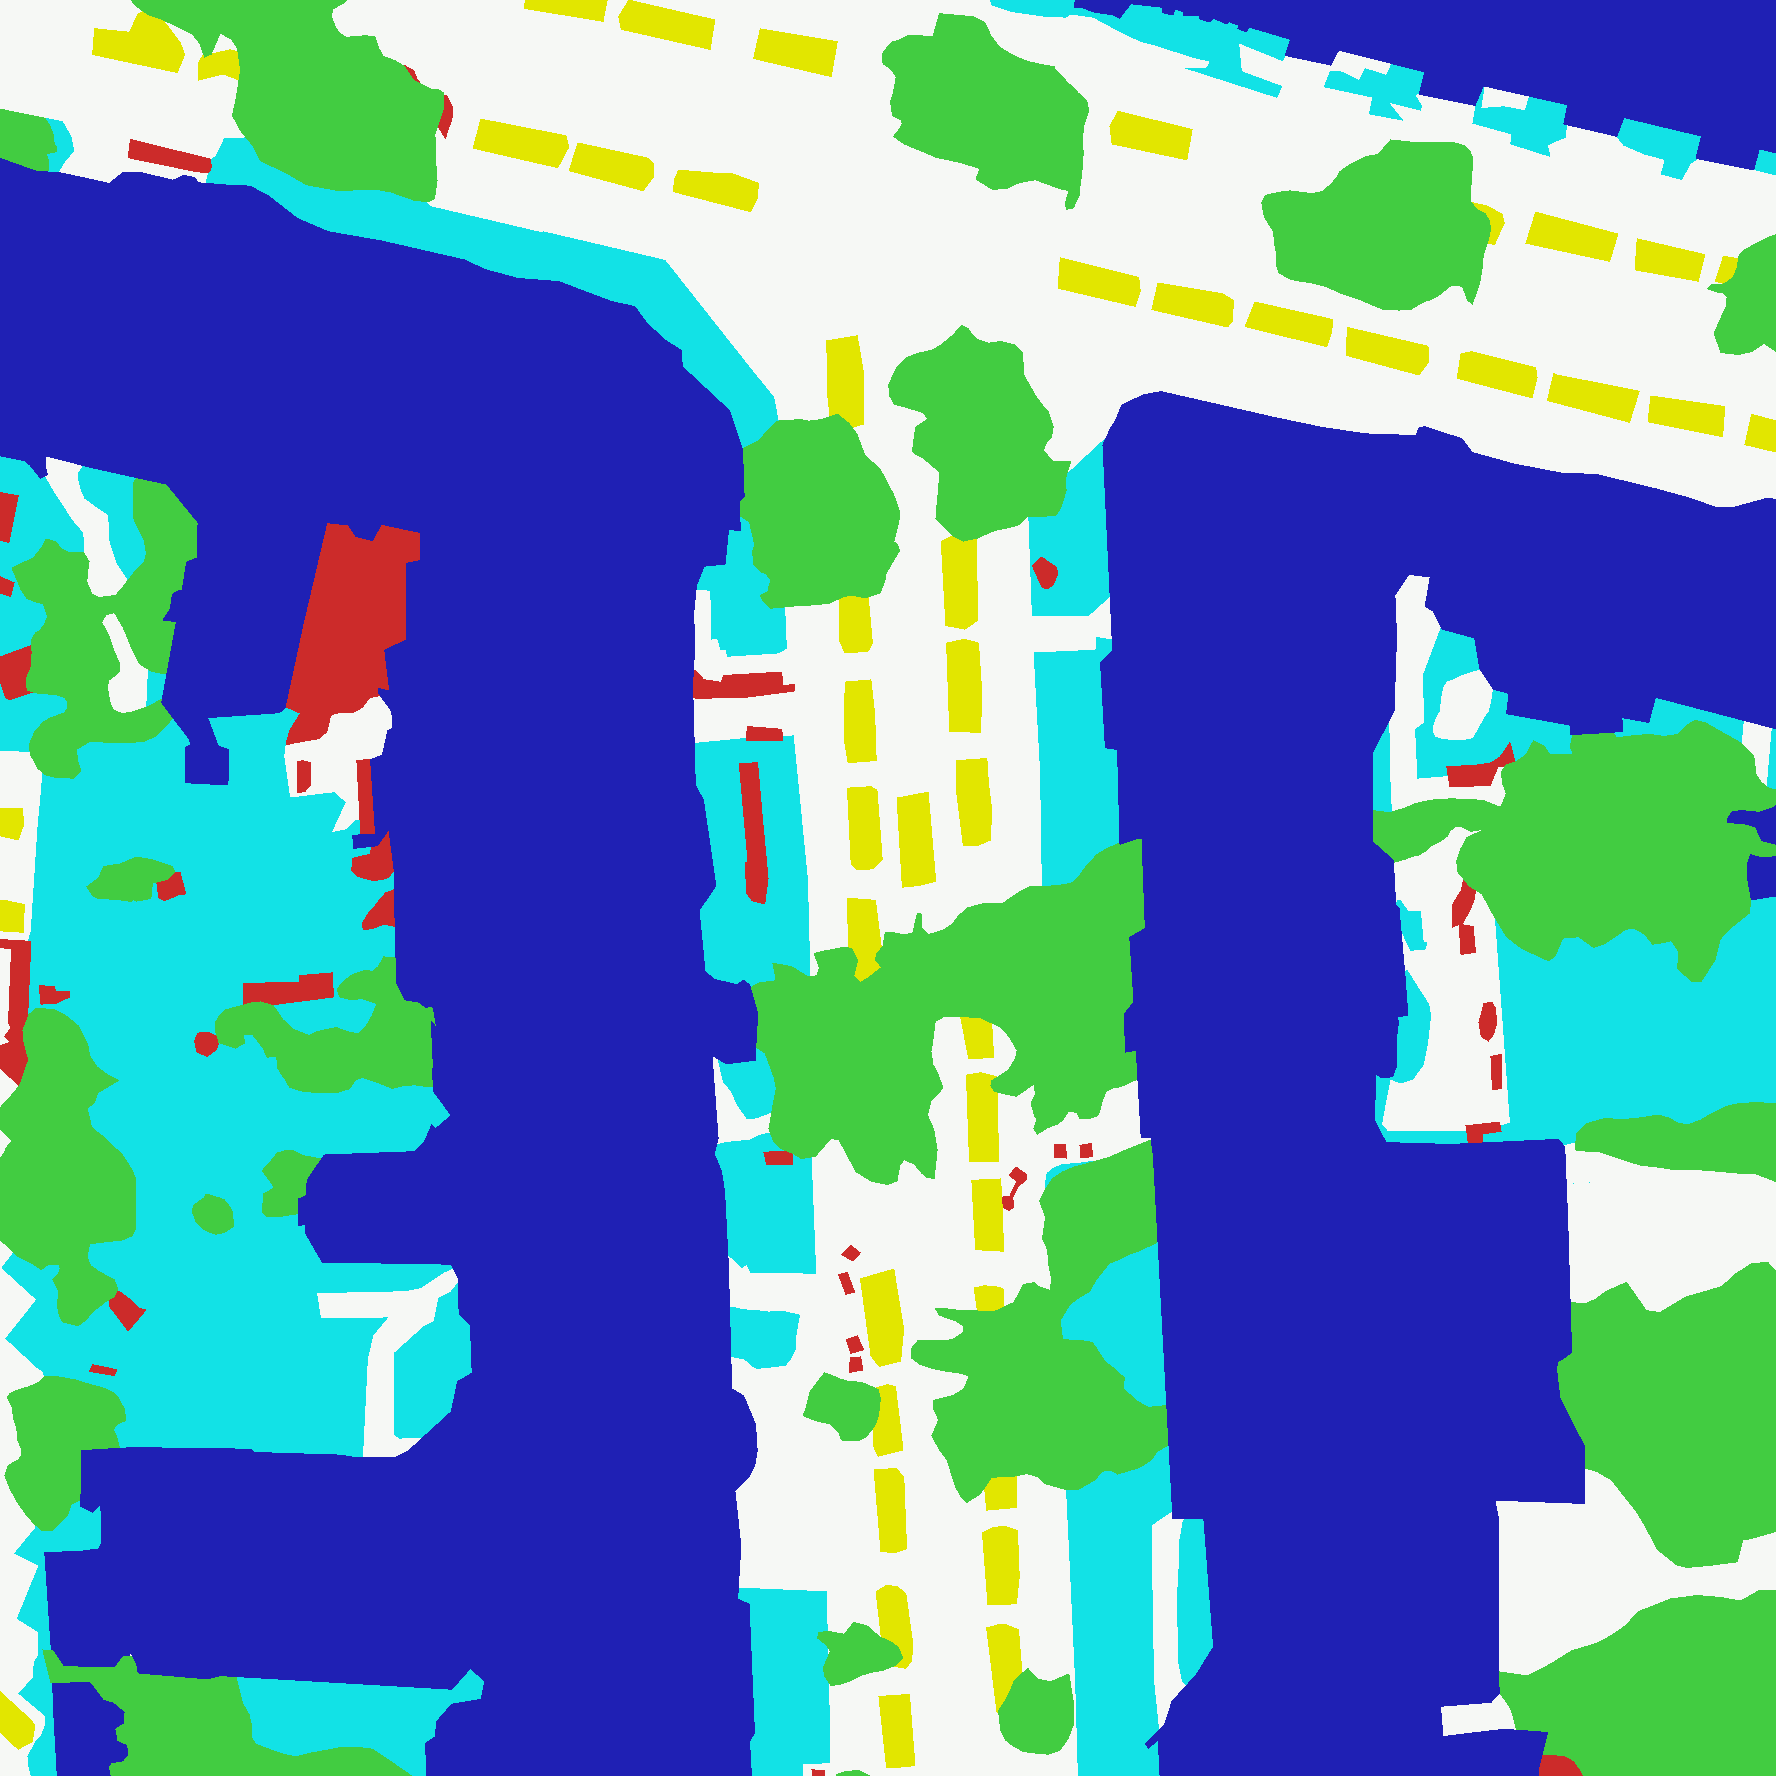
\includegraphics[width=5.5cm]{../Chapitre2/potsdam_sample_gt}};
    \node [transform shape, rotate=-90, below] at (output.west) {\huge{Segmentation}};
    \end{scope}

\newcommand\legendlayer[3]{%{name}{x}{color}
\convlayer{0.1*\scale}{0.1*\scale}{0.2*\scale}{}{#3}{#2}{-1.6*\scale}{0}{}
\node[anchor=west] at (#2+0.125*\scale, -1.6*\scale) {\large = #1};
}
\legendlayer{convolution + BN + ReLU}{0.5*\scale}{blue}
\legendlayer{\emph{maxpooling}}{2*\scale}{yellow}
\legendlayer{\emph{unpooling}}{3*\scale}{red}
\legendlayer{fusion (concaténation)}{4*\scale}{cyan}



\end{tikzpicture}


\end{document}
}
    \caption{Correction résiduelle appliquée à SegNet.}
    \label{fig:residual_correction}
\end{figure}

Une approche alternative consiste à séparer les traitements appliqués aux différentes modalités et à combiner les prédictions de l'ensemble des modèles. Ainsi, il est envisageable d'entraîner un modèle par modalité et de réaliser la moyenne des prédiction. Toutefois, cela ne permet pas de prendre en compte les particularités de chaque capteur. Nous introduisons donc un module de correction résiduelle qui prend en entrée les dernières cartes d'activation des réseaux et réalise une fusion des cartes de probabilités~\cite{audebert_semantic_2016}. Le module de correction résiduelle apprend la correction $\epsilon$ à appliquer à la prédiction moyenne pour améliorer les performances globales du modèle combiné. Ce processus est illustré dans la~\cref{fig:residual_correction} pour SegNet.

Ce module réalise une fusion au niveau décisionnel en utilisant le principe de l'apprentissage résiduel~\cite{he_deep_2016}. Il comporte trois couches convolutives de noyau $3\times3$ et un \emph{padding} de \SI{1}{\px}. Les cartes d'activation intermédiaires des deux décodeurs de SegNet sont concaténées et utilisées comme entrées pour le module de correction (cf. \cref{fig:residual_correction}). La sortie du module est sommée de façon résiduelle avec la moyenne de prédictions issues des SegNet, comme illustré dans la~\cref{fig:correction_network}. Dans ce cas, l'apprentissage par résidu est particulièrement adapté car la prédiction moyenne peut déjà être considérée comme proche du résultat visé. Le module additionnel vient donc fusionner les décisions en appliquant une moyenne pondérée adaptative dépendant des cartes d'activations afin d'ajouter un terme correctif à la prédiction moyenne. Ce module, entraîné par rétropropagation, est simplement optimisé \emph{a posteriori} par \emph{fine-tuning}, les SegNet n'étant pas ré-entraînés. Ce procédé est donc rapide, car seuls les gradients sur les couches du module correctif sont calculés.

%Let $M_r$ denote the input of the $r^{th}$ stream ($r \in \{1,\dots,R\}$ with $R = 2$ here), $P_{r}$ the output probability tensor and $Z_r$ the intermediate feature map used for the correction. The corrected prediction is:

% \begin{equation}
% P'(M_1, \dots, M_R) = P(M_1, \dots, M_R) + correction(Z_1, \dots, Z_R)
% \end{equation}
% where
% \begin{equation}
% P(M_1, \dots, M_n) = \frac{1}{R}\sum_{r=1}^R P_r(M_r)~.
% \end{equation}

Notons $P_\mathit{terrain}$ le tenseur représentant la vérité terrain et $\hat{P}_i$ les prédictions réalisées par la $i$\ieme sortie. On définit alors le terme d'erreur $\epsilon_i$ tel que\,:
\begin{equation}
\hat{P}_i = P_\mathit{terrain} + \epsilon_i \text{~~~avec~~~} \lvert \epsilon_i \lvert ~\ll~ \rvert \hat{P}_i \rvert~~.
\end{equation}

Si la prédiction $P_i$ est relativement, alors $\epsilon_i$ reste faible. L'objectif du module de correction résiduelle est d'apprendre à estimer l'erreur afin de pouvoir la corriger lors de l'inférence.

En notant $n$ le nombre de prédictions à fusionner par correction résiduelle, alors la sortie du module notée $\hat{P}^*$ correspond à la somme de la prédiction moyenne des $\hat{P}_i$ et d'un terme correcteur $c$\,:
\begin{equation}
\hat{P}^* = \hat{P}_\mathit{moyenne} + c = \frac{1}{n} \sum_{i=1}^n P_i + c = P_\mathit{terrain} + \frac{1}{n} \sum_{i=1}^n \epsilon_i + c~~.
\label{eq:residual_correction}
\end{equation}

Le module de correction résiduelle étant optimisé pour la minimiser la fonction de coût, cette contrainte se traduit par\,:
\begin{equation}
\left\lVert \hat{P}^* - P_\mathit{terrain} \right\rVert \rightarrow 0
\end{equation}
ce qui impose en retour la contrainte suivante sur $c$ et $\epsilon_i$\,:
\begin{equation}
\left\lVert \frac{1}{n} \sum_{i=1}^n \epsilon_i - c \right\rVert \rightarrow 0~~.
\end{equation}

\begin{figure}[t]
  \centering
  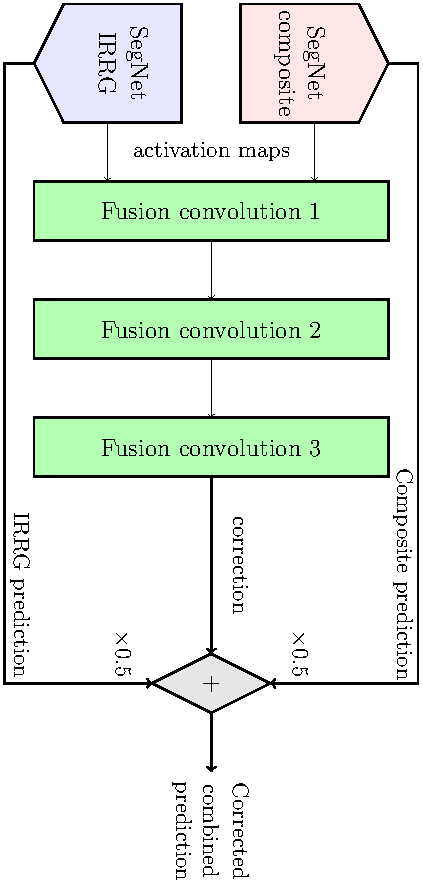
\includegraphics[height=0.9\textwidth,angle=90]{correct_network}
  \caption{Module de correction résiduelle.}
  \label{fig:correction_network}
\end{figure}

Autrement dit, le module de correction résiduelle est optimisé afin de compenser l'erreur moyenne commise par les différents modèles de l'ensemble. Lors de la phase d'entraînement, la vérité terrain $P_\mathit{terrain}$ est connue. Les poids du module sont alors altérés par rétro-propagation de sorte que le terme correctif $c$ se rapproche de $\sum_{i=1}^n \epsilon_i$. L'erreur moyenne étant supposée faible, la correction d'erreur correspond ainsi au paradigme d'apprentissage par résidu~\cite{he_deep_2016}. En effet, $c$ est un terme additif de faible amplitude sommé au signal initial (ou \emph{bypass}). Cette approche est schématisée dans la~\cref{fig:correction_network}.

\subsection{Résultats expérimentaux}

\todo[inline]{Hyperparamètres}

\begin{table}
    \caption{Résultats de segmentation sémantique multi-modale sur le jeu de test \glsname{ISPRS} Vaihingen.}
    \label{table:final_vaihingen}
    \setlength\tabcolsep{5pt}
	\begin{tabularx}{\textwidth}{Y c c c c c c}
    \toprule
	  Modèle & routes & bâtiments & vég. basse & arbres & véhicules & Exactitude\\
    \midrule
    FCN~\cite{sherrah_fully_2016} & 90.5 & 93.7 & 83.4 & 89.2 & 72.6 & 89.1\\
    FCN + fusion + frontières~\cite{marmanis_classification_2017} & \textbf{92.3} & \textbf{95.2} & 84.1 & \textbf{90.0} & 79.3 & \textbf{90.3}\\
    \midrule
    SegNet (\glssymbol{IRRV}) & 91.5 & 94.3 & 82.7 & 89.3 & 85.7 & 89.4\\
	  SegNet-RC & 91.0 & 94.5 & 84.4 & 89.9 & 77.8 & 89.8\\
    FuseNet & 91.3 & 94.3 & \textbf{84.8} & 89.9 & 85.9 & 90.1\\
    V-FuseNet & 91.0 & 94.4 & 84.5 & 89.9 & \textbf{86.3} & 90.0\\
    \bottomrule
    \end{tabularx}
\end{table}

\begin{table}
    \caption{Résultats de segmentation sémantique multi-modale sur le jeu de test \glsname{ISPRS} Potsdam.}
    \label{table:final_potsdam}
    \setlength\tabcolsep{4pt}
	\begin{tabularx}{\textwidth}{Y c c c c c c}
    \toprule
  	Modèle & routes & bâtiments & vég. basse & arbres & véhicules & Exactitude\\\\
    \midrule
    FCN + CRF + caractéristiques expertes~\cite{liu_dense_2017} & 91.2 & 94.6 & 85.1 & 85.1 & 92.8 & 88.4\\
    FCN~\cite{sherrah_fully_2016} & 92.5 & \textbf{96.4} & 86.7 & 88.0 & 94.7 & 90.3\\
    \midrule
    SegNet (\glssymbol{IRRV}) & 92.4 & 95.8 & 86.7 & 87.4 & 95.1 & 90.0\\
	  SegNet-RC & 91.3 & 95.9 & 86.2 & 85.6 & 94.8 & 89.0\\
    V-FuseNet & \textbf{92.7} & 96.3 & \textbf{87.3} & \textbf{88.5} & \textbf{95.4} & \textbf{90.6}\\
    \bottomrule
    \end{tabularx}
\end{table}


\begin{figure}[!tb]
	\begin{subfigure}{\textwidth}
    	\captionsetup[subfigure]{singlelinecheck=off,justification=centering}
  		\captionsetup[subfigure]{labelformat=empty}
    	\begin{subfigure}{0.19\textwidth}
        	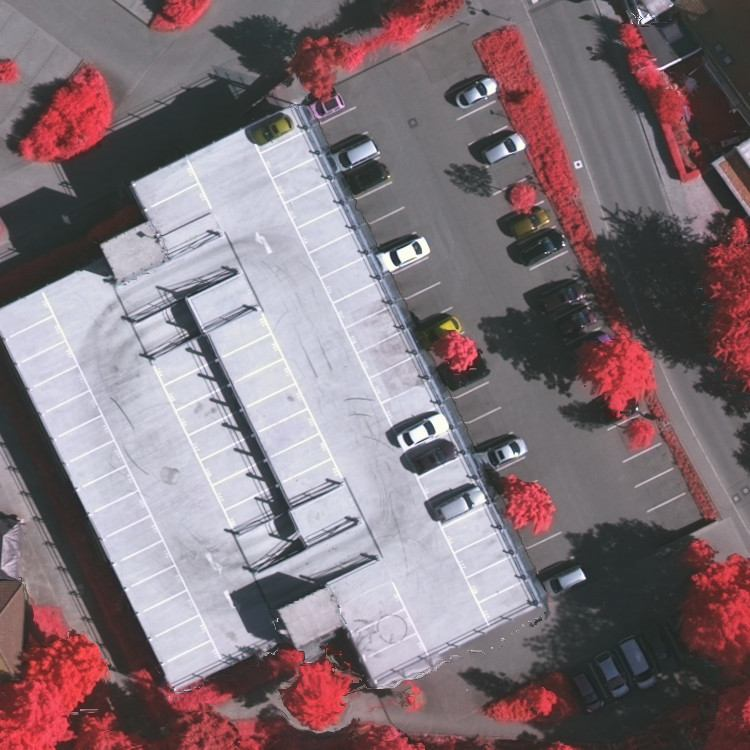
\includegraphics[width=\textwidth]{tile5_irrg_top}
      		\caption*{Image \glssymbol{IRRV}}
        \end{subfigure}
        \begin{subfigure}{0.19\textwidth}
        	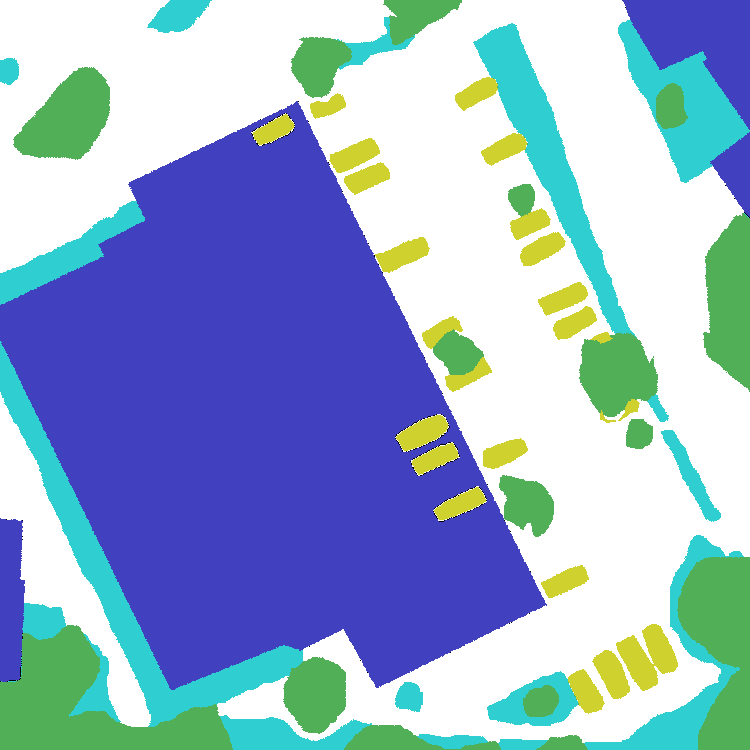
\includegraphics[width=\textwidth]{tile5_gt}
        	\caption*{Vérité terrain}
        \end{subfigure}
        \begin{subfigure}{0.19\textwidth}
        	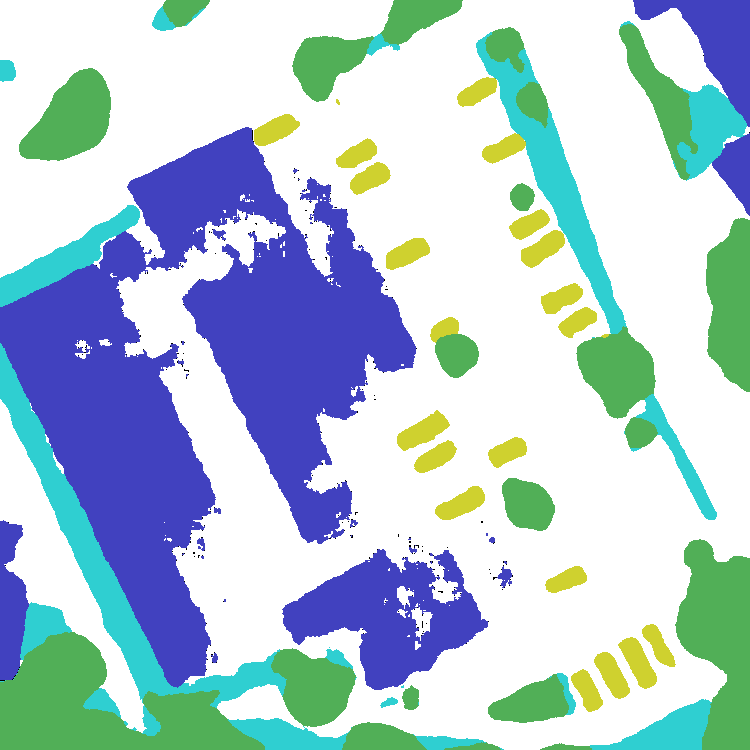
\includegraphics[width=\textwidth]{tile5_segnet_pred}
        	\caption*{SegNet}
        \end{subfigure}
        \begin{subfigure}{0.19\textwidth}
        	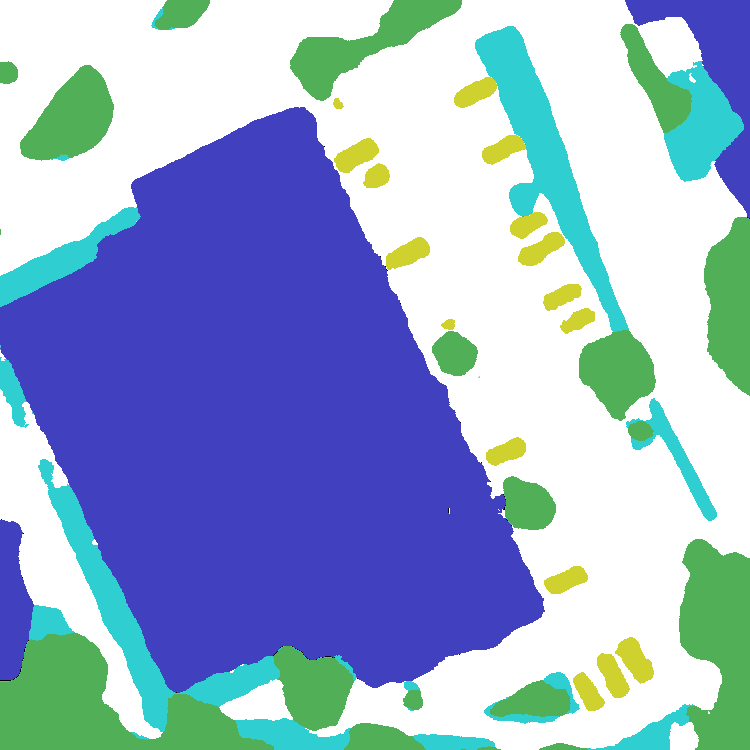
\includegraphics[width=\textwidth]{tile5_fusenet_pred}
        	\caption*{FuseNet}
        \end{subfigure}
        \begin{subfigure}{0.19\textwidth}
        	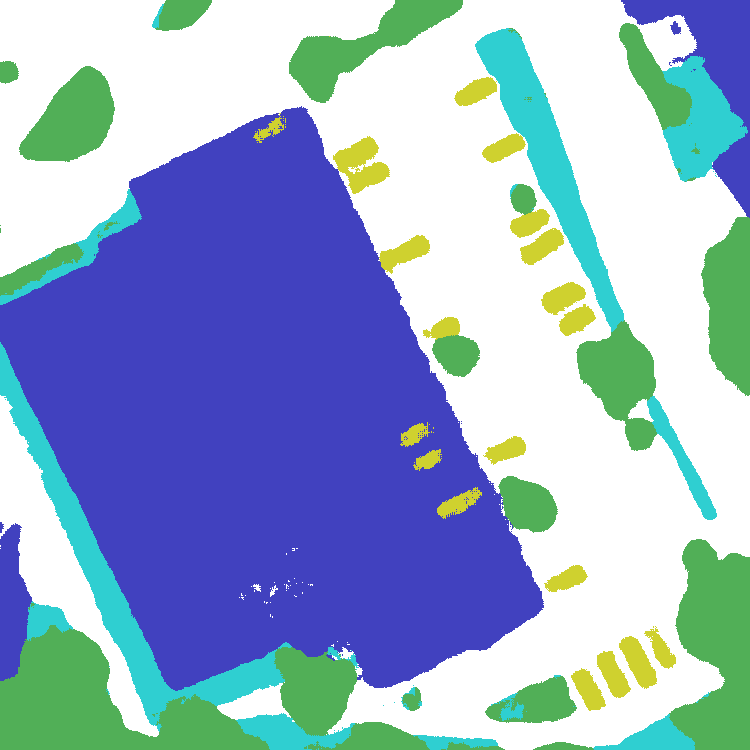
\includegraphics[width=\textwidth]{tile5_rc_pred}
        	\caption*{SegNet-CR}
        \end{subfigure}
        \caption{Prédictions de différentes modèles sur un extrait du jeu de données \glsname{ISPRS} Vaihingen.}
        \label{fig:fusion_exemple1}
    \end{subfigure}
    	\begin{subfigure}{\textwidth}
    	\captionsetup[subfigure]{singlelinecheck=off,justification=centering}
  		\captionsetup[subfigure]{labelformat=empty}
    	\begin{subfigure}{0.19\textwidth}
        	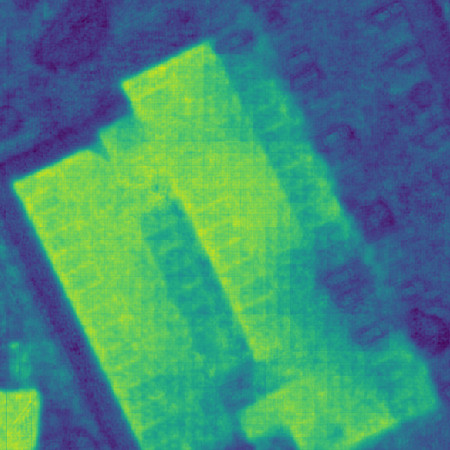
\includegraphics[width=\textwidth]{tile5_irrg_confidence_buildings}
      		\caption*{SegNet \glssymbol{IRRV} (confiance, bâtiments)}
        \end{subfigure}
        \begin{subfigure}{0.19\textwidth}
        	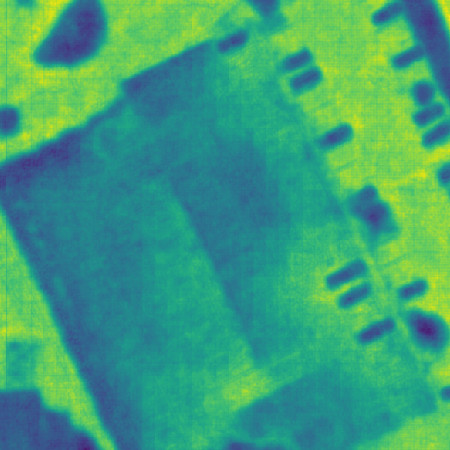
\includegraphics[width=\textwidth]{tile5_irrg_confidence_roads}
        	\caption*{SegNet \glssymbol{IRRV} (confiance, routes)}
        \end{subfigure}
        \begin{subfigure}{0.19\textwidth}
        	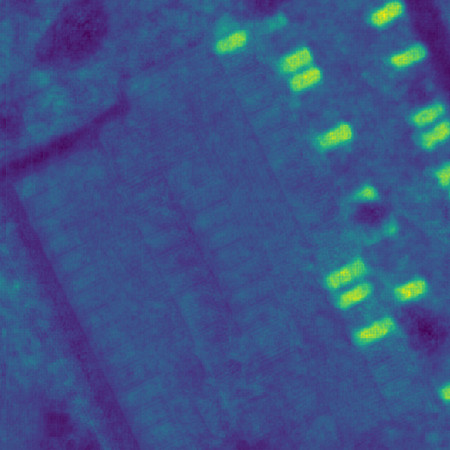
\includegraphics[width=\textwidth]{tile5_irrg_confidence_cars}
        	\caption*{SegNet \glssymbol{IRRV} (confiance, voitures)}
        \end{subfigure}
        \begin{subfigure}{0.19\textwidth}
        	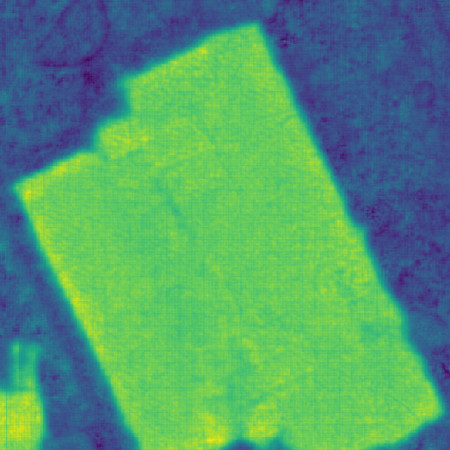
\includegraphics[width=\textwidth]{tile5_comp_confidence_buildings}
        	\caption*{SegNet composite (confiance, bâtiments)}
        \end{subfigure}
        \begin{subfigure}{0.19\textwidth}
        	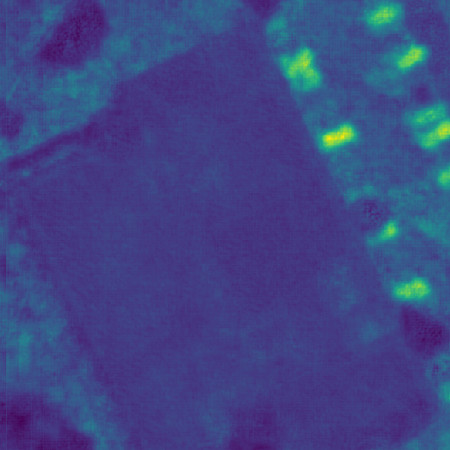
\includegraphics[width=\textwidth]{tile5_comp_confidence_cars}
        	\caption*{SegNet composite (confiance, voitures)}
        \end{subfigure}
        \caption{Cartes de confiance de SegNet pour diverses classes selon le type d'entrée.}
        \label{fig:confidence_vaihingen_fusion}
    \end{subfigure}
    \begin{subfigure}{\textwidth}
    	\captionsetup[subfigure]{singlelinecheck=off,justification=centering}
  		\captionsetup[subfigure]{labelformat=empty}
    	\begin{subfigure}{0.19\textwidth}
        	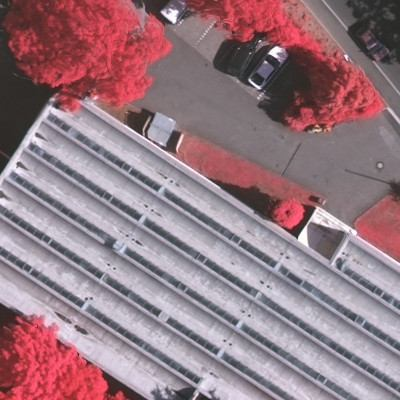
\includegraphics[width=\textwidth]{tile21_irrg_top}
      		\caption*{Image \glssymbol{IRRV}}
        \end{subfigure}
        \begin{subfigure}{0.19\textwidth}
        	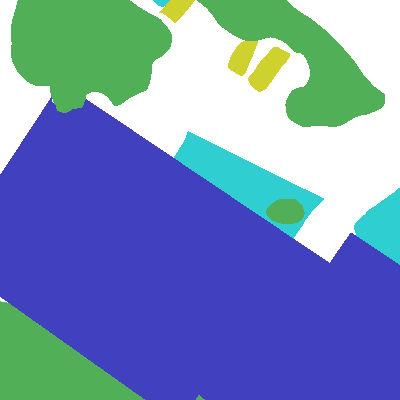
\includegraphics[width=\textwidth]{tile21_gt}
        	\caption*{Vérité terrain}
        \end{subfigure}
        \begin{subfigure}{0.19\textwidth}
        	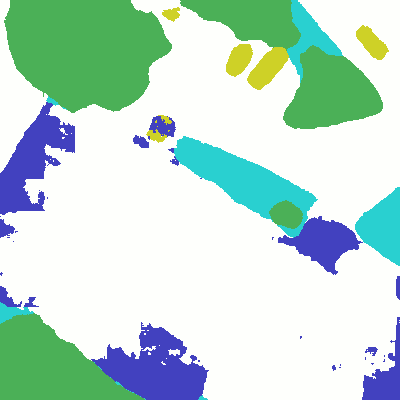
\includegraphics[width=\textwidth]{tile21_segnet_pred}
        	\caption*{SegNet}
        \end{subfigure}
        \begin{subfigure}{0.19\textwidth}
        	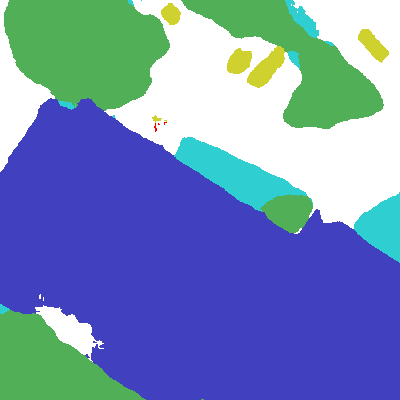
\includegraphics[width=\textwidth]{tile21_fusenet_pred}
        	\caption*{FuseNet}
        \end{subfigure}
        \begin{subfigure}{0.19\textwidth}
        	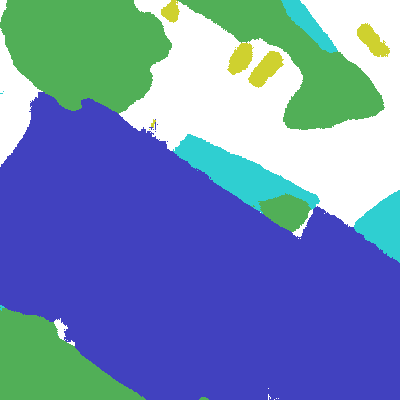
\includegraphics[width=\textwidth]{tile21_rc_pred}
        	\caption*{SegNet-CR}
        \end{subfigure}
        \caption{Prédictions de différentes modèles sur un extrait du jeu de données \glsname{ISPRS} Vaihingen.}
        \label{fig:fusion_exemple2}
    \end{subfigure}

	\caption[Prédiction réussies à l'aide des stratégies de fusion.]{Prédiction réussies à l'aide des stratégies de fusion.\\
  \isprslegende}
   	\label{fig:fusion_success}
\end{figure}

\begin{figure}[h]
	\begin{subfigure}{0.32\textwidth}
    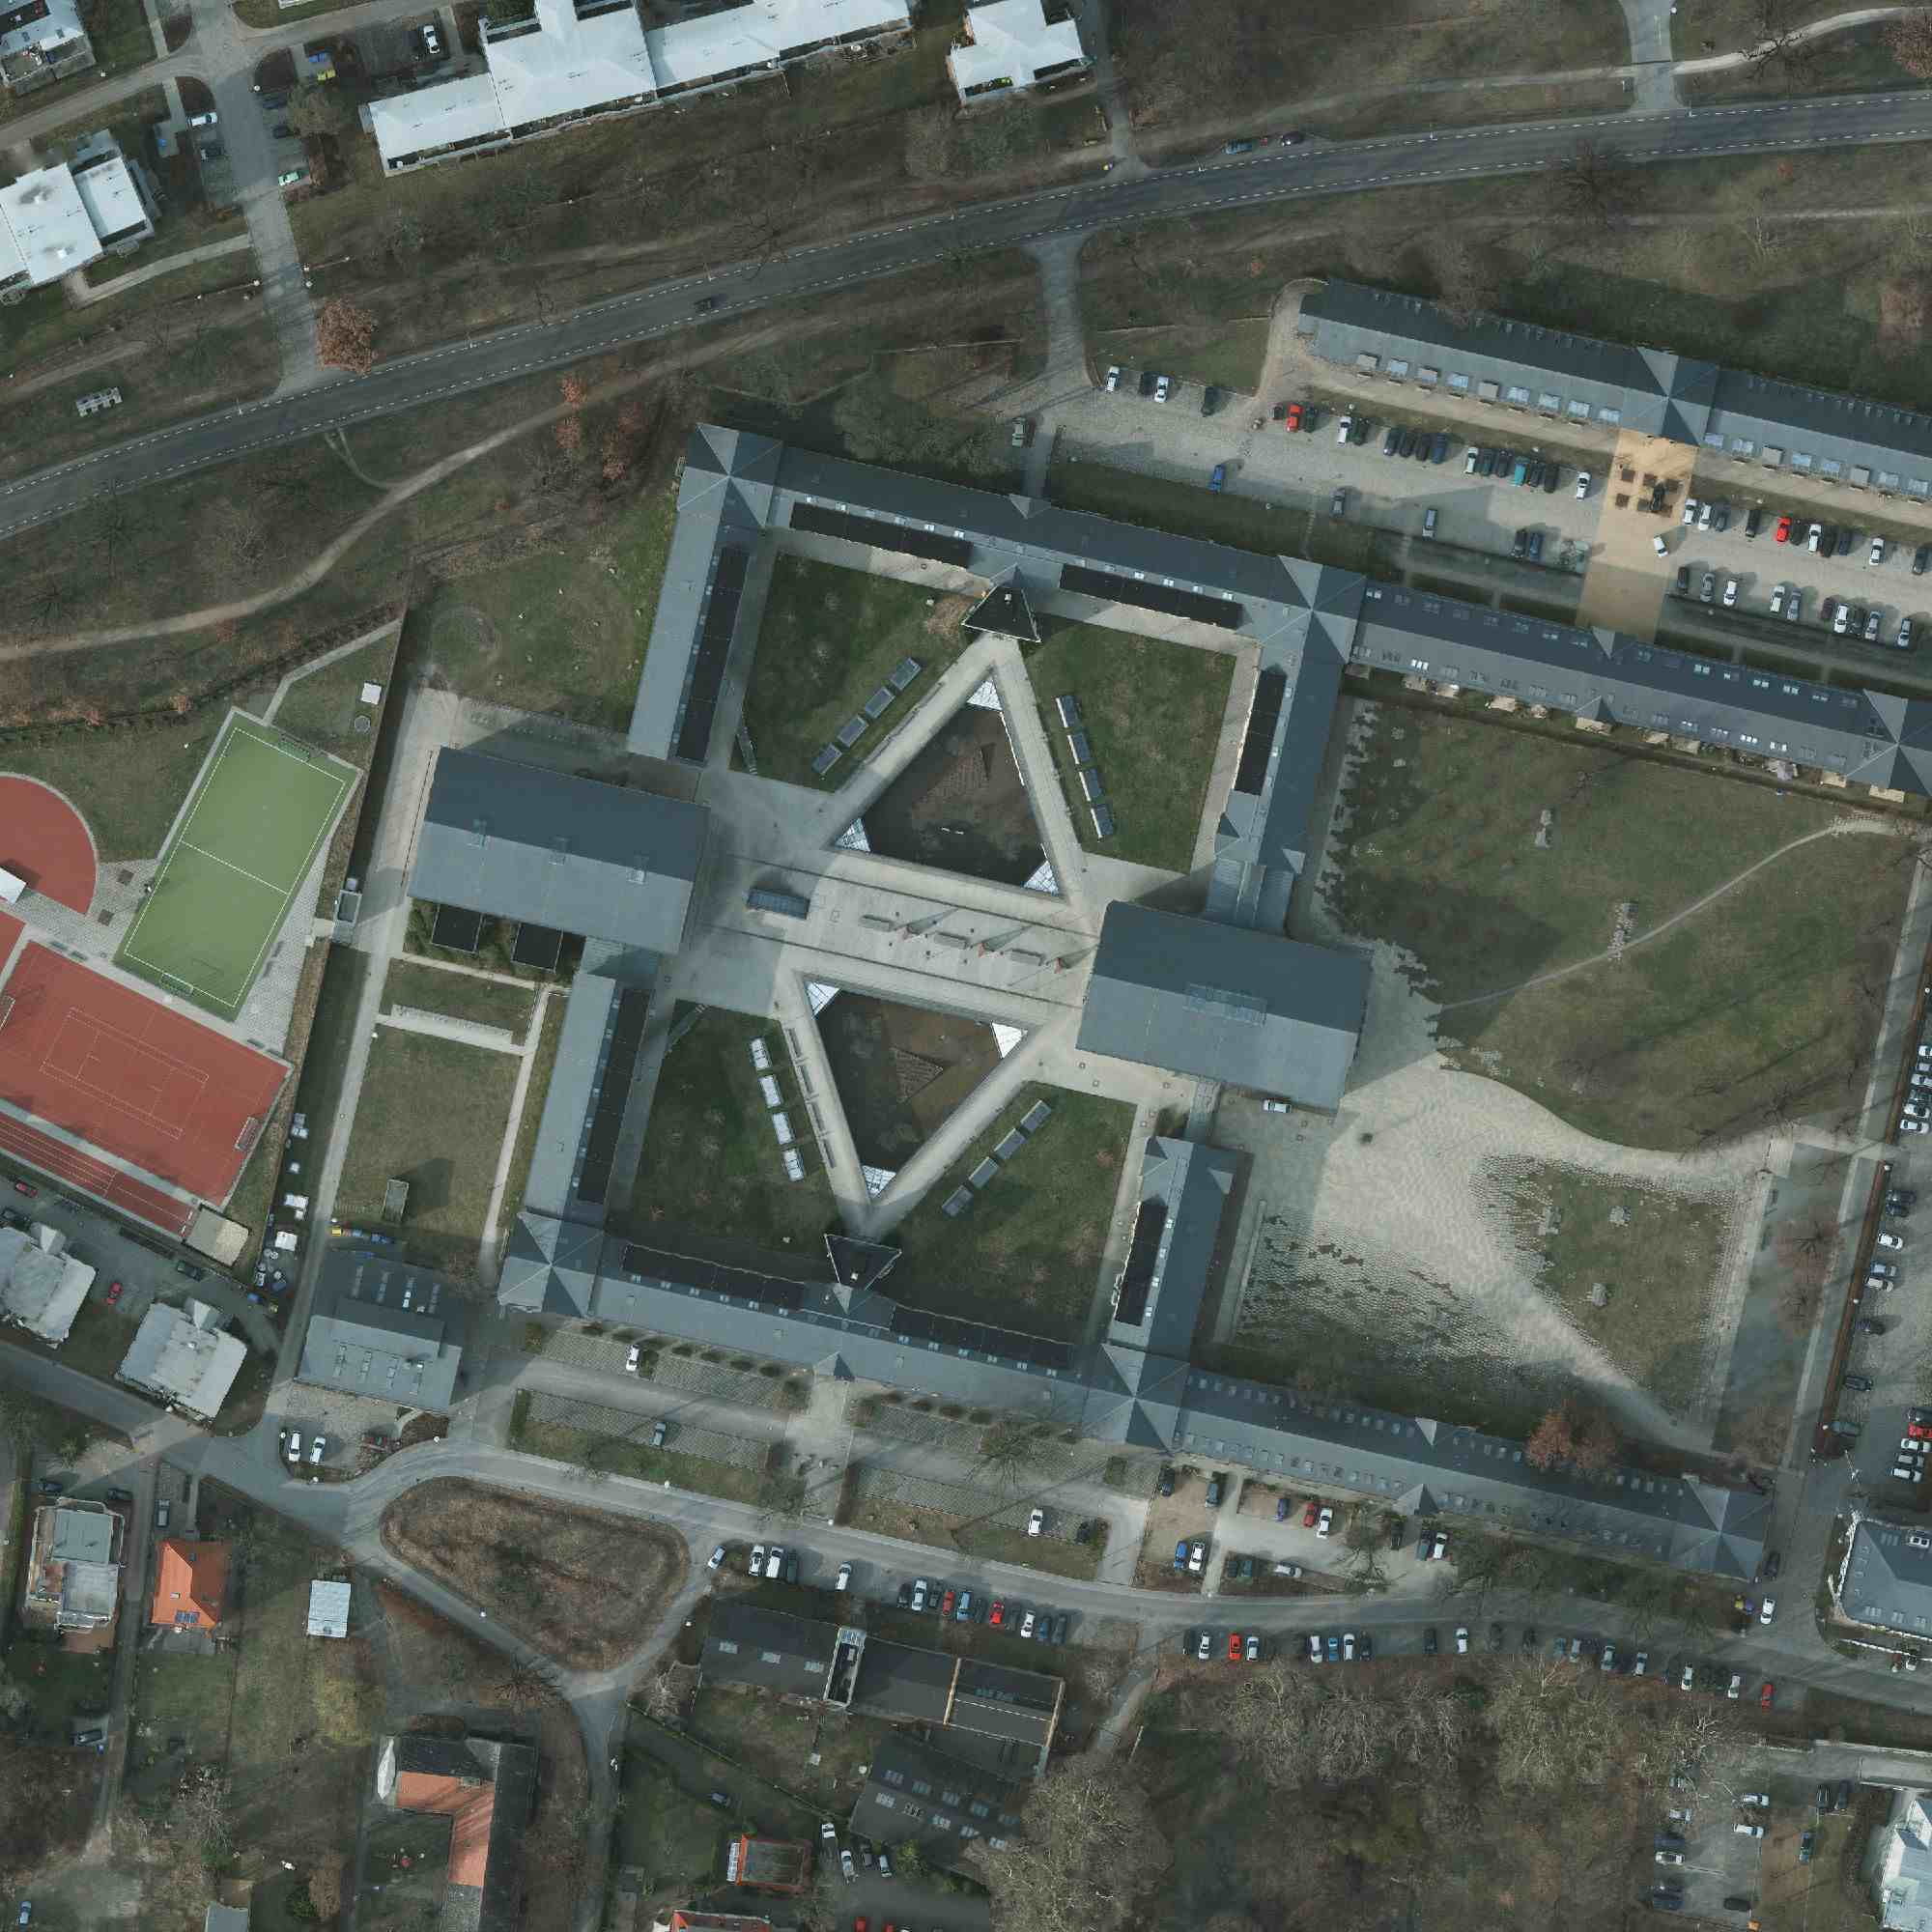
\includegraphics[width=\linewidth]{potsdam_rgb_3_11}
    \caption{Image \glssymbol{RVB}}
    \end{subfigure}
    \begin{subfigure}{0.32\textwidth}
    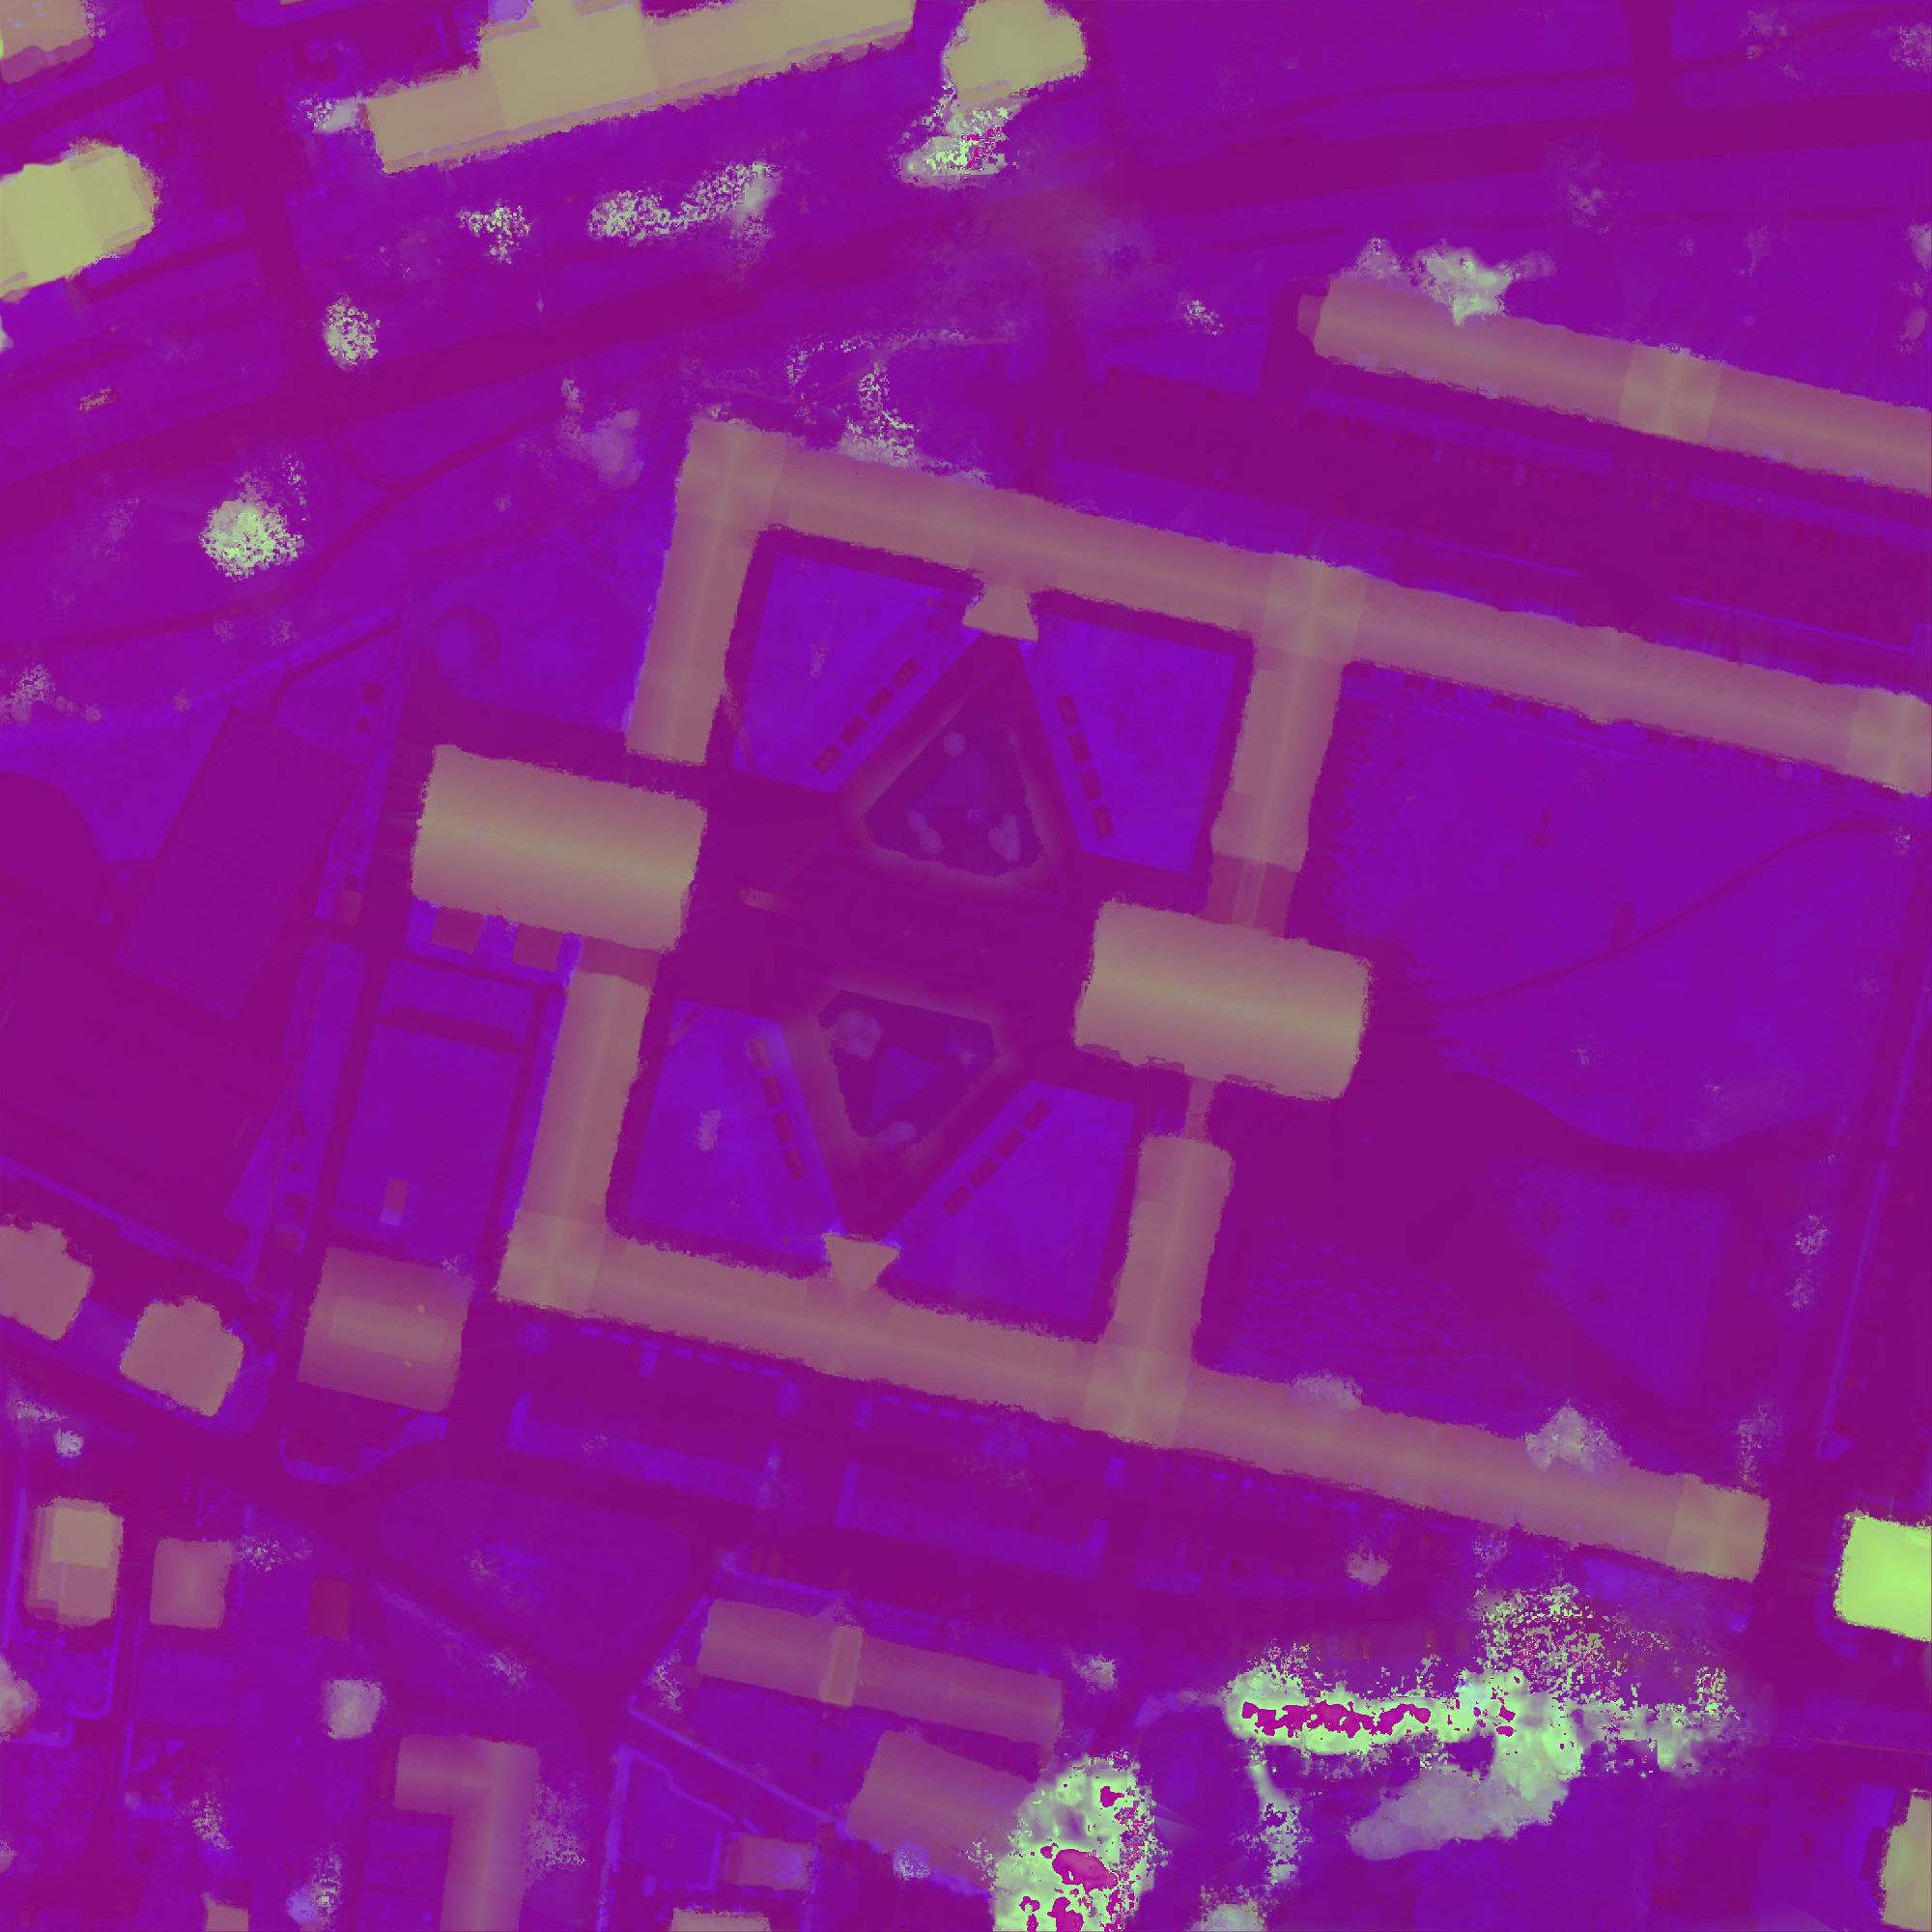
\includegraphics[width=\linewidth]{potsdam_comp_3_11}
    \caption{Image composite}
    \end{subfigure}
    \begin{subfigure}{0.32\textwidth}
    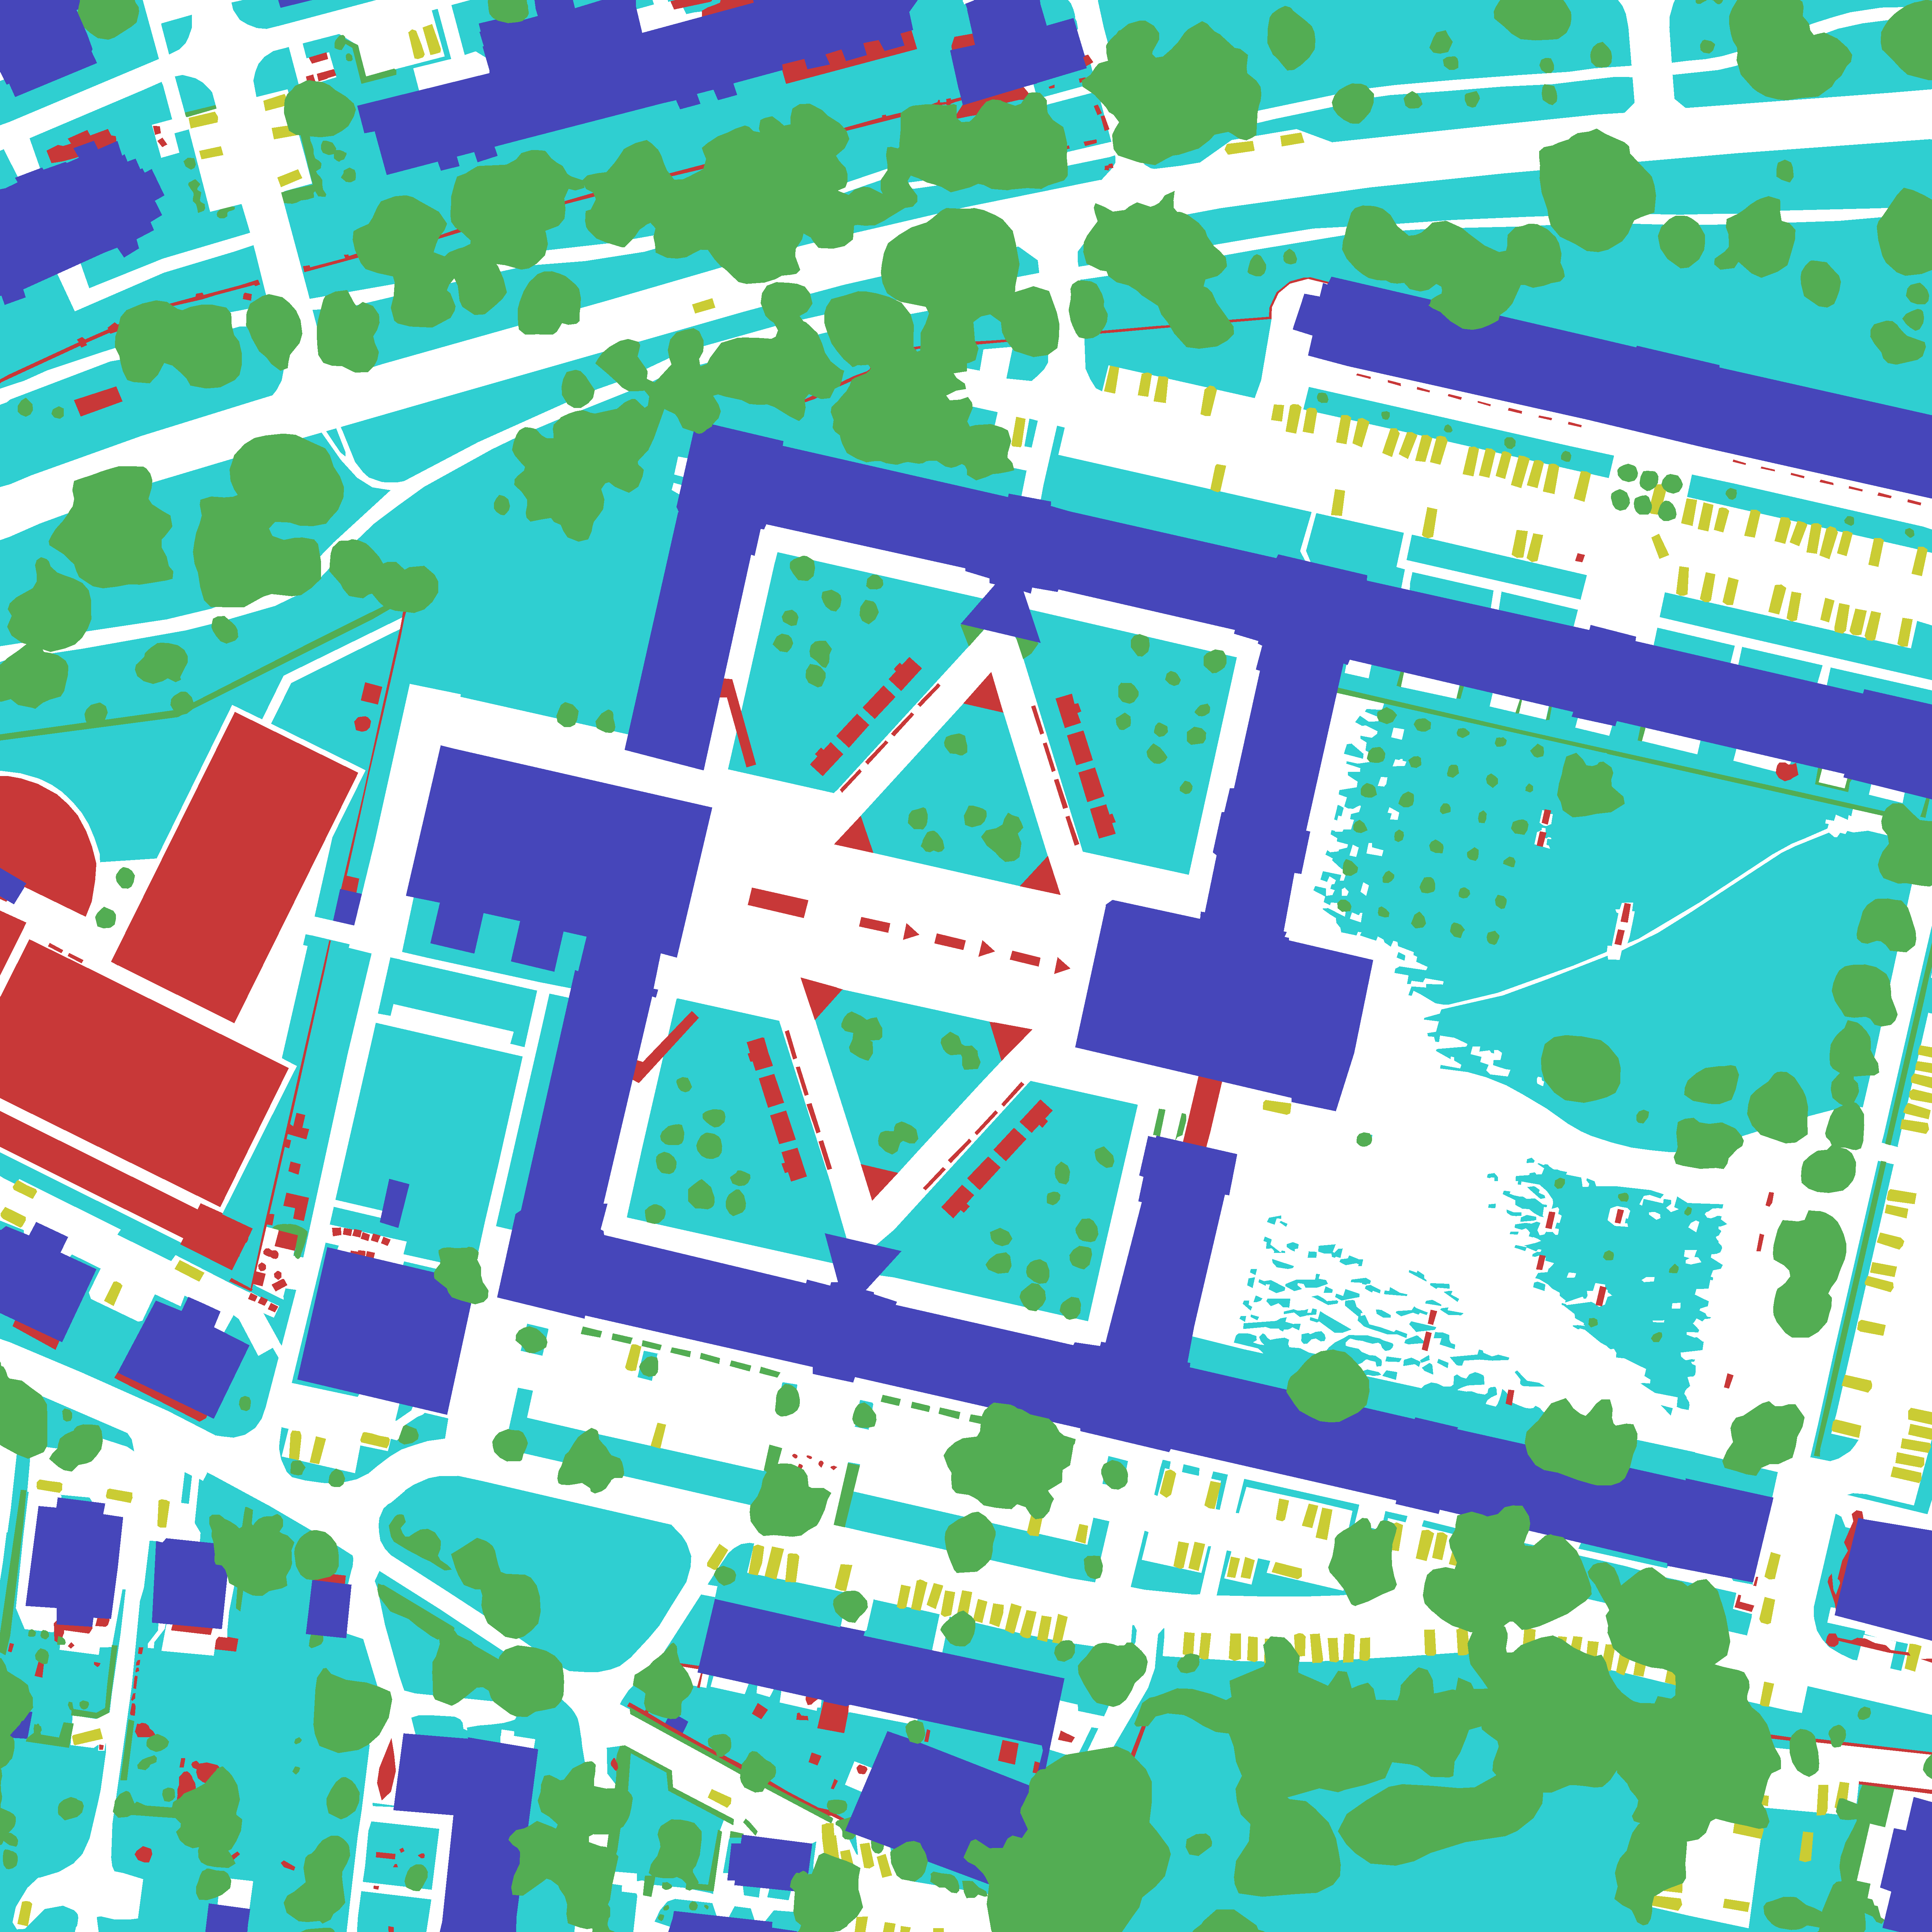
\includegraphics[width=\linewidth]{potsdam_gt_3_11}
    \caption{Vérité terrain}
    \end{subfigure}
    \begin{subfigure}{0.49\textwidth}
    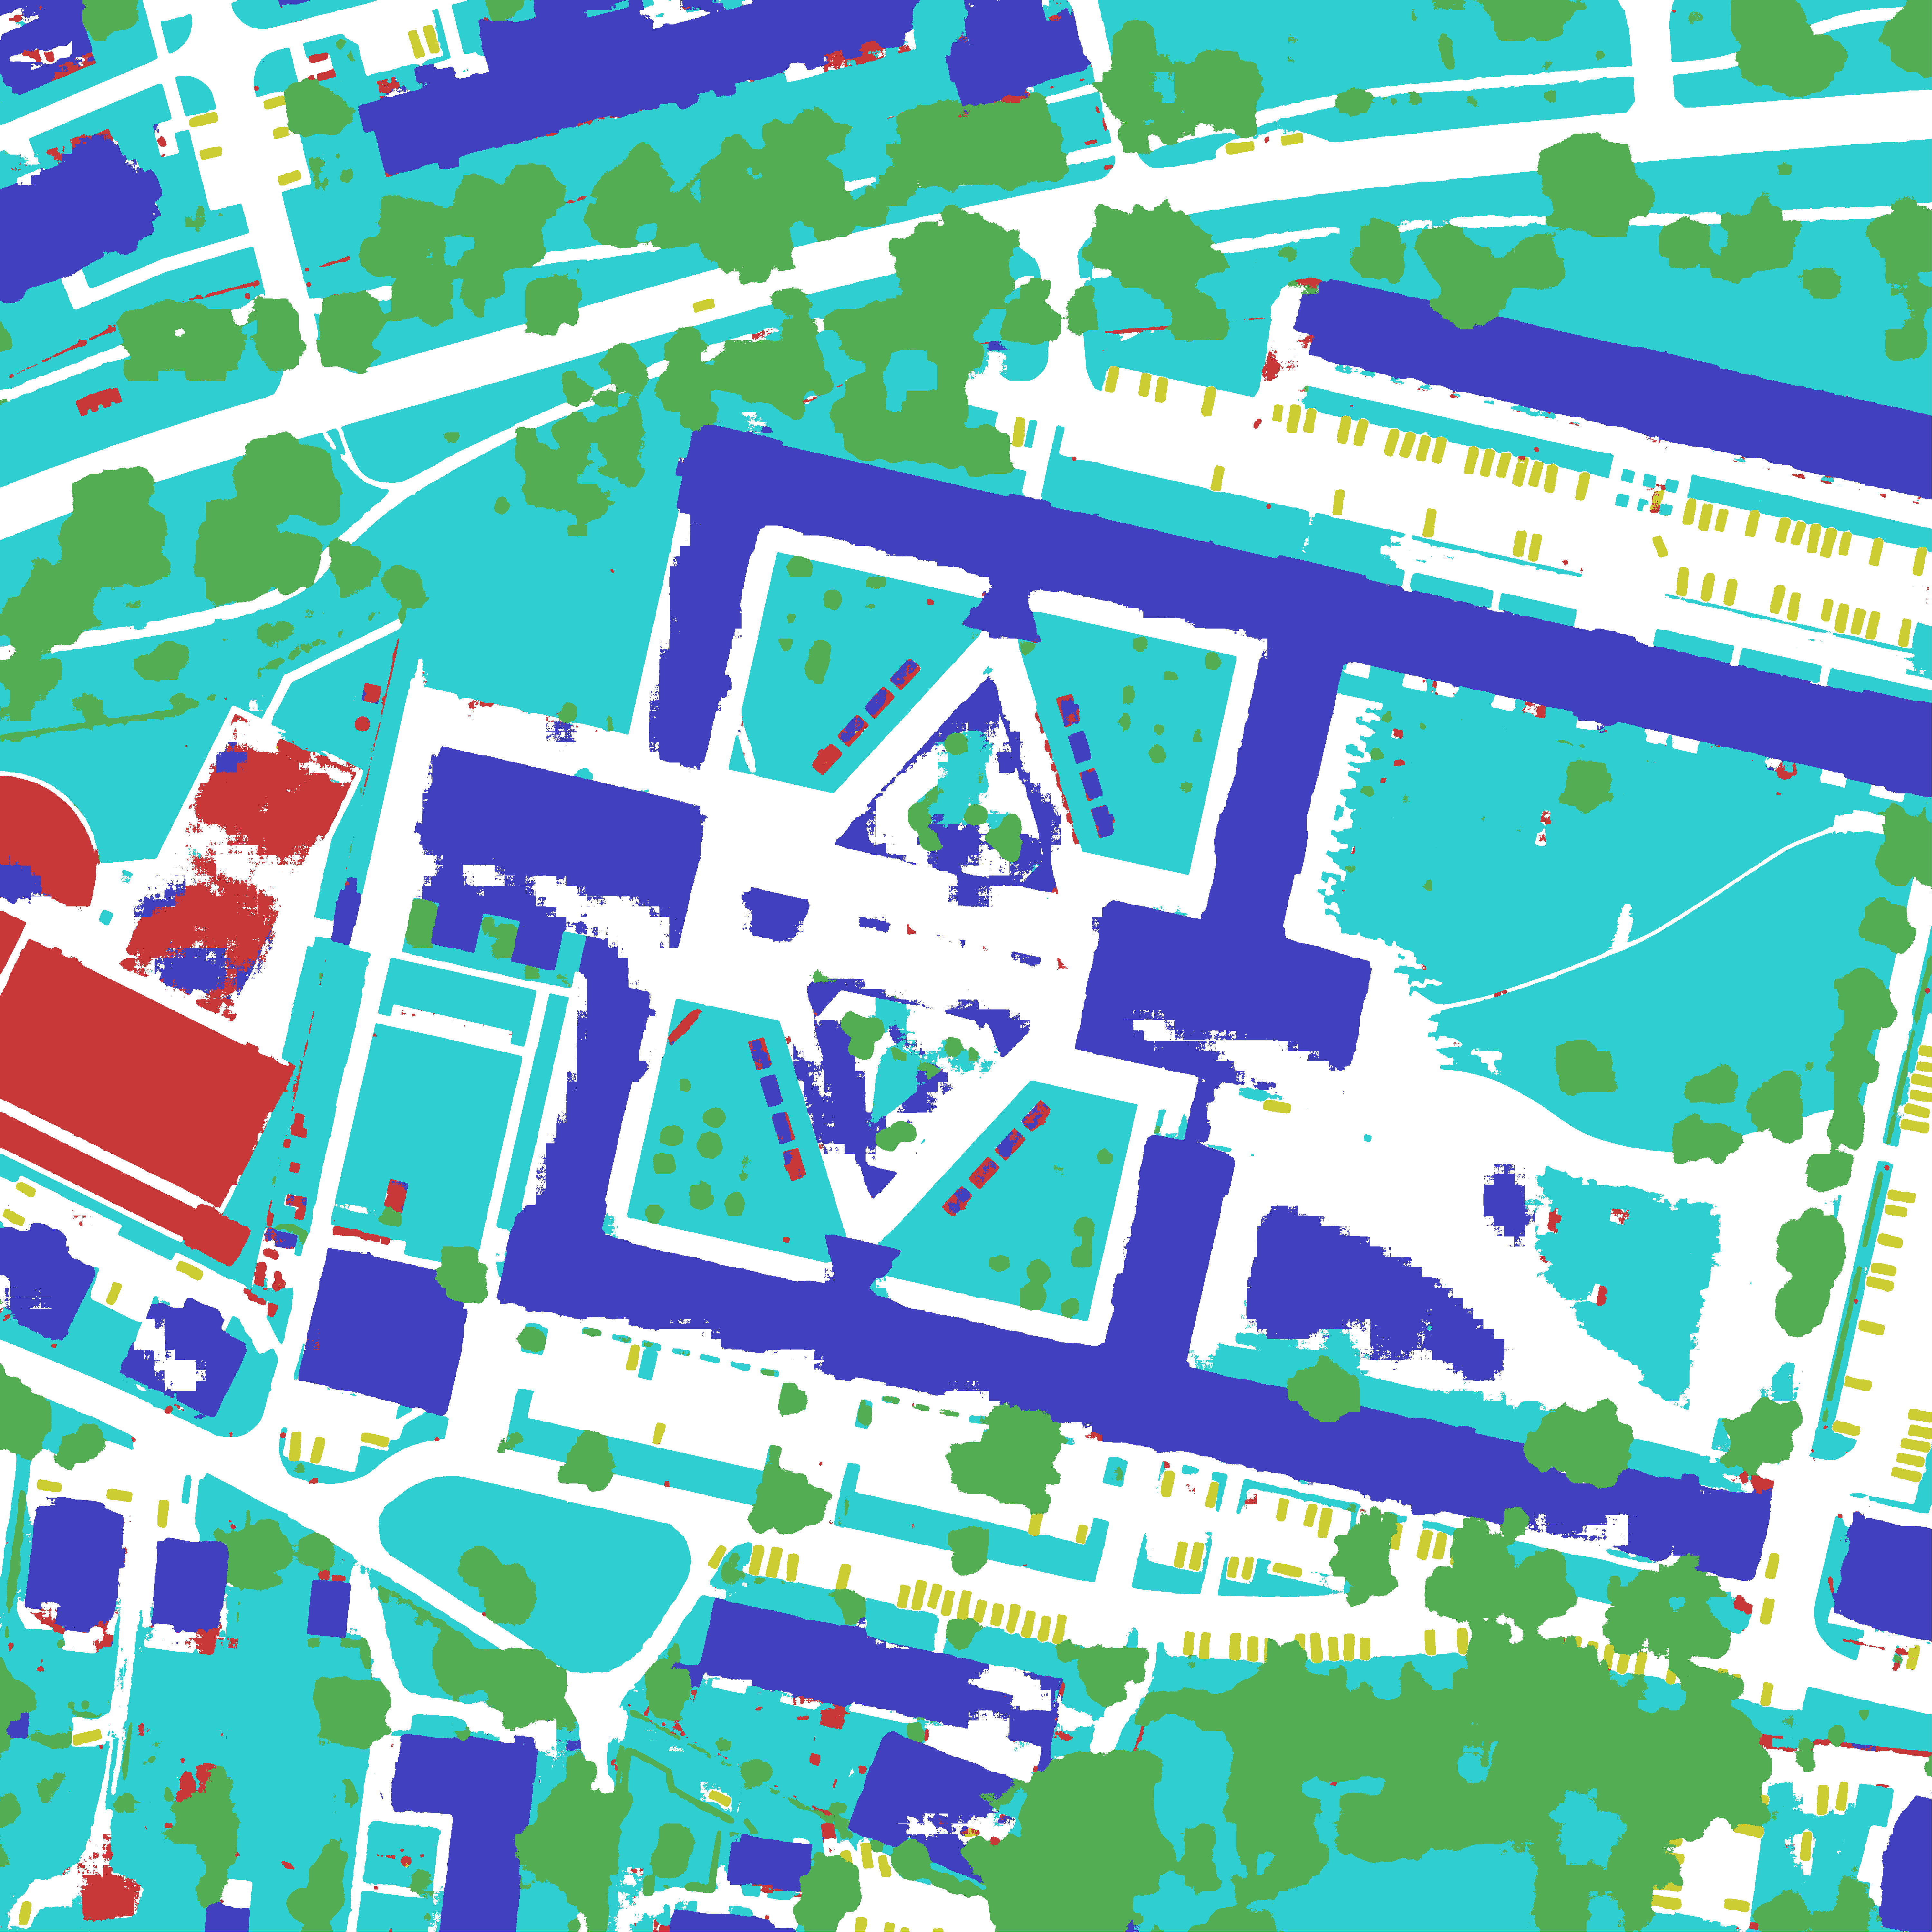
\includegraphics[width=\linewidth]{segnet_irrg_potsdam_3_11}
    \caption{SegNet}
    \end{subfigure}
    \begin{subfigure}{0.49\textwidth}
    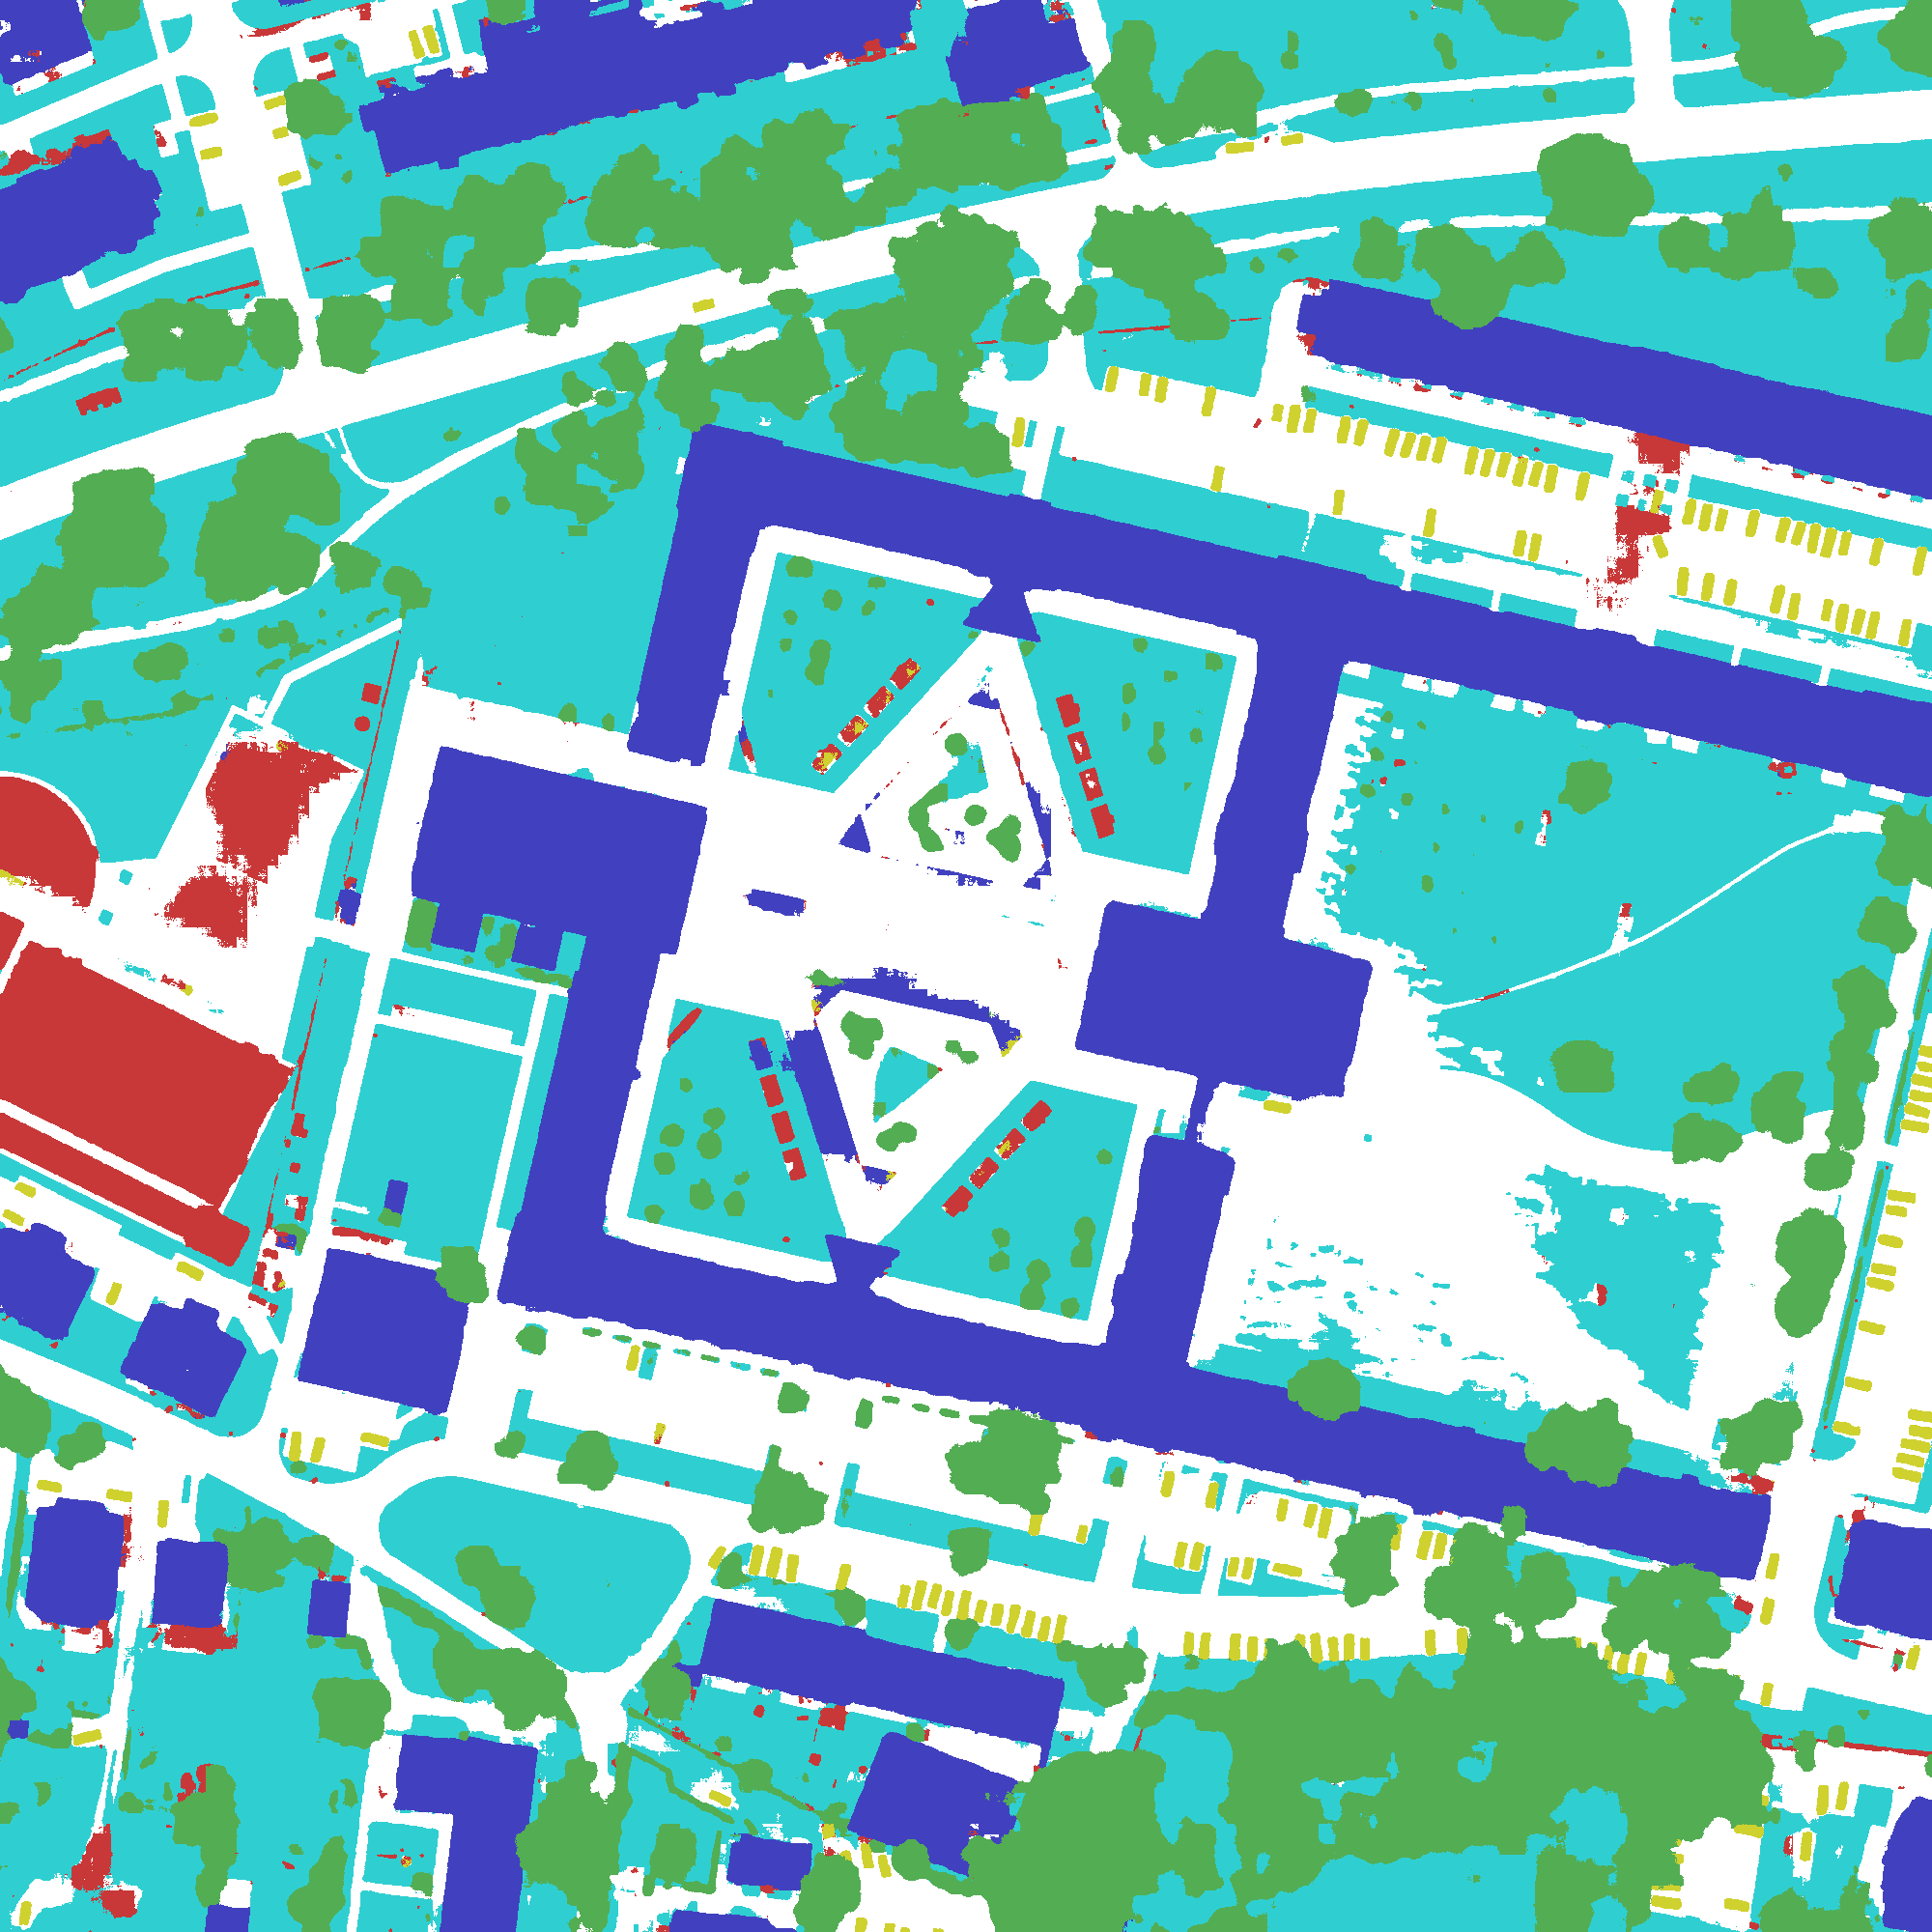
\includegraphics[width=\linewidth]{fusenet_irrg_comp_potsdam_3_11}
    \caption{V-FuseNet}
    \end{subfigure}
    \caption[Effet des stratégies de fusion sur un extrait du jeu de données \glsname{ISPRS} Potsdam.]{Effet des stratégies de fusion sur un extrait du jeu de données \glsname{ISPRS} Potsdam. La confusion entre les classes de route et de bâtiments est nettement réduite grâce à la contribution des modèles de terrain.\\\isprslegende}
    \label{fig:potsdam_images}
\end{figure}

Comme attendu, les deux méthodes de fusion permettent d'améliorer les performances du classifieur sur les deux jeux de données, comme illustré par les~\cref{fig:fusion_exemple1,fig:potsdam_images}. En particulier, la~\cref{fig:fusion_success} montre plusieurs exemples d'objets erronnément classifiés à partir de l'image optique seule qui sont corrigés en intégrant l'image composite dans le modèle. Dans les~\cref{fig:fusion_exemple1,fig:confidence_vaihingen_fusion}, le réseau SegNet ne parvient pas à discriminer entre les classes de route et de bâtiment, compte-tenu du fait qu'il s'agit d'un parking aérien à l'apparence proche de ceux pouvant se trouver au sol, confusion renforcée par la présence des voitures. FuseNet utilise le \gls{MNH} pour trancher en faveur de la classe bâtiment et ignore de fait les véhicules. L'approche par correction résiduelle parvient en plus à conserver une partie de l'information spatiale liée aux voitures. Dans la~\cref{fig:fusion_exemple2}, SegNet confond également route et bâtiment et végétation haute et basse tandis que les deux architectures de fusion parviennent à correctement prédire les différentes objets grâce au \gls{MNH}.
%As expected, both fusion methods improve the classification accuracy on the two datasets, as illustrated in~\cref{fig:potsdam_images}. We show some examples of misclassified patches that are corrected using the fusion process in~\cref{fig:fusion_success}. In~\cref{fig:fusion_exemple1,fig:confidence_vaihingen_fusion}, SegNet is confused by the material of the building and the presence of cars. However, FuseNet uses the nDSM to decide that the structure is a building and ignore the cars, while the late fusion manages to mainly to recover the cars. This is similar to~\cref{fig:fusion_exemple2}, in which SegNet confuses the building with a road while FuseNet and the residual correction recover the information thanks to the nDSM both for the road and the trees in the top row.
La fusion dans l'encodeur par FuseNet permet d'exploiter conjointement les modalités multiples en utilisant moins de paramètres que la correction résiduelle d'un ensemble de modèles et converge vers une meilleure performance globale. À l'opposé, la fusion tardive par correction résiduelle améliore les performances de manière moins équilibrée, les gains étant principalement concentrés sur les classes ``routes'' et ``bâtiments''.
%One advantage of using the early fusion is that complementarity between the multiple modalities is leveraged more efficiently as it requires less parameters, yet achieves a better classification accuracy for all classes. At the opposite, late fusion with residual correction improves the overall accuracy at the price of less balanced predictions. Indeed, the increase mostly affects the ``building'' and ``impervious surface'' classes, while all the other F1 scores decrease slightly.

\begin{table}
    \caption{Résultats de segmentation sémantique multi-modale sur le jeu de validation \glsname{ISPRS} Vaihingen.}
    \label{table:val_vaihingen}
	\begin{tabularx}{\textwidth}{Y c c}
    \toprule
    Modèle & Exactitude & Score $F_1$\\
    \midrule
    SegNet (\glssymbol{IRRV}) & 90.2 {\small $\pm$ 1.4} & 89.3 {\small $\pm$ 1.2}\\
    SegNet (composite) & 88.3 {\small $\pm$ 0.9} & 81.6 {\small $\pm$ 0.8}\\
    SegNet-CR & 90.6 {\small $\pm$ 1.4} & 89.2 {\small $\pm$ 1.2}\\
    FuseNet & 90.8 {\small $\pm$ 1.4} & 90.1 {\small $\pm$ 1.2}\\
    V-FuseNet & \textbf{91.1} {\small $\pm$ 1.5} & \textbf{90.3} {\small $\pm$ 1.2}\\
    \midrule
    ResNet-34 (\glssymbol{IRRV}) & 90.3 {\small $\pm$ 1.0} & 89.1 {\small $\pm$ 0.7}\\
    ResNet-34 (composite) & 88.8 {\small $\pm$ 1.1} & 83.4 {\small $\pm$ 1.3}\\
    ResNet-34-CR & 90.8 {\small $\pm$ 1.0} & 89.1 {\small $\pm$ 1.1}\\
    FusResNet & 90.6 {\small $\pm$ 1.1} & 89.3 {\small $\pm$ 0.7}\\
    \bottomrule
    \end{tabularx}
\end{table}


En outre, la correction résiduelle est moins utile lorsque la confiance accordée par les modèles dans leurs prédictions est faible. Sur le jeu de données \gls{ISPRS} Potsdam, le SegNet composite n'atteint que 79\% de taux de bonne classification, car l'image composite est moins informative pour discriminer des objets à résolution de \SI{5}{\centi\meter/\px}. Par conséquent, la correction résiduelle dégrade légèrement les performances. En revanche, sur le jeu de données \gls{ISPRS} Vaihingen, l'image composite est nettement plus informative (85\% de taux de bonne classification) et l'ensemble parvient à combiner efficacement les deux sources de données car les deux sont informatives avec un bon taux de confiance, comme illustré dans la~\cref{fig:confidence_vaihingen_fusion}. On observe par ailleurs qu'améliorer les performances sur l'image composite en utilisant un ResNet-34 permet également d'améliorer la performance de la correction résiduelle.
%\todo{mesurer le gain théorique union entre les deux sources de données}
%However, on the Potsdam dataset, the residual correction strategy slightly decreases the model accuracy. Indeed, the late fusion is mostly useful to combine strong predictions that are complementary. For example, as illustrated in~\cref{fig:confidence_vaihingen_fusion}, the composite SegNet has a strong confidence in its building prediction while the IRRG SegNet has a strong confidence in its cars predictions. Therefore, the residual correction is able to leverage those predictions and to fuse them to alleviate the uncertainty around the cars in the rooftop parking lot. This works well on Vaihingen as both the IRRG and composite sources achieve a global accuracy higher than 85\%. However, on Potsdam, the composite SegNet is less informative and achieves only 79\% accuracy, as the annotations are more precise and the dataset overall more challenging for a data source that relies only on Lidar and NDVI. Therefore, the residual correction fails to make the most of the two data sources. This analysis is comforted by the fact that, on the Vaihingen validation set, the residual correction achieves a better global accuracy with ResNets than with SegNets, thanks to the stronger ResNet-34 trained on the composite source.

L'architecture FuseNet apprend une représentation conjointe des deux sources de données, mais fait face aux même problématiques que le modèle SegNet standard\,: les cas rares comme les voitures sur un toit sont incorrectement prédits. Les caractéristiques conjointes apprises par les deux encodeurs sont plus performantes, mais FuseNet reste sensible au sur-apprentissage et aux biais intrinsèques du jeu de données, là où la correction résiduelle parvient à corriger des erreurs même sur des cas rares.

%Meanwhile, the FuseNet architecture learns a joint representation of the two data sources, but faces the same pitfall as the standard SegNet model : edge cases such as cars on rooftop parking lots disappear. However, the joint-features are significantly stronger and the decoder can perform a better classification using this multi-modal representation, therefore improving the global accuracy of the model.
La fusion tardive est ainsi pertinente lorsqu'il s'agit de combiner des prédictions fortement complémentaires et agit comme une moyenne pondérée adaptative des prédictions. Pour les cas du parking aérien, la prédiction du SegNet composite prédit un bâtiment avec une confiance haute car le \gls{MNH} est fiable, tandis que le SegNet \gls{RVB} produit des prédictions à fort niveau de confiance sur les voitures. À l'inverse, FuseNet apprend représentations conjointes qui n'échappent pas au surapprentissage. Ainsi, les voitures sur le parking aérien disparaissent à l'inférence car c'est un cas unique au sein du jeu de données\,: les voitures sont normalement sur la route.
%Sur Vaihingen, ça marche bien car le composite et l'IRRG donnent à peu près la même quantité d'info (les deux modèles sont à au moins 85\%). Par contre sur Potsdam, la fusion tardive ne marche pas terrible, car le composite est à 79\% et a tendance à être moins informatif (surtout que les annotations sur Potsdam sont bien plus précises). Donc la fusion tardive va plutôt galérer. Il me semble qu'on retrouve quand même le même phénomène de véhicules sur le toit, il faut que je retrouve la tuile concernée.}

En conclusion, ces deux stratégies de fusion sont applicables à différentes cas d'utilisation. La fusion tardive par correction résiduelle est utile pour combiner des classifieurs forts très complémentaires, tandis que la stratégie FuseNet est plus adaptée pour exploiter de l'information annexe ancillaire dans le processus d'apprentissage.
%In conclusion, the two fusion strategies can be used for different use cases. Late fusion by residual correction is more suited to combine several strong classifiers that are confident in their predictions, while the FuseNet early fusion scheme is more adapted for integrating weaker ancillary data into the main learning pipeline.

%\todo{Explanation for V-FuseNet (visual if possible)}
Sur le jeu de test final de Vaihingen (cf.~\cref{tab:final_vaihingen}), la stratégie V-FuseNet a des performances marginalement inférieures au modèle original, bien que les $F_1$ scores soient supérieurs sur certaines classes, y compris la classe de rejet ($+1,7\%$) qui n'est pas prise en compte dans les métriques finales.

\subsubsection{Robustesse aux données manquantes}

\begin{figure}[h]
	\captionsetup[subfigure]{singlelinecheck=off,justification=centering}
    \captionsetup[subfigure]{labelformat=empty}
    \begin{subfigure}{0.24\textwidth}
    	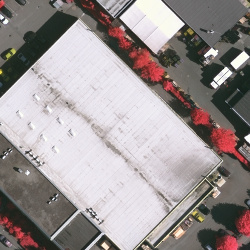
\includegraphics[width=\textwidth]{ndsm_fail_top}
        \caption{\glssymbol{IRRV}}
    \end{subfigure}
    \begin{subfigure}{0.24\textwidth}
    	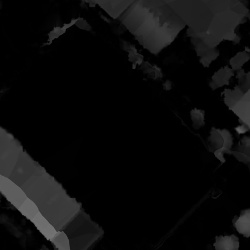
\includegraphics[width=\textwidth]{ndsm_fail_ndsm}
        \caption{\glssymbol{MNH}}
    \end{subfigure}
    \begin{subfigure}{0.24\textwidth}
    	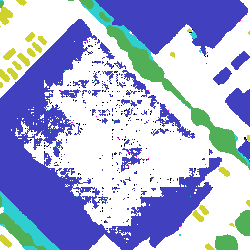
\includegraphics[width=\textwidth]{ndsm_fail_residual}
        \caption{SegNet-CR}
    \end{subfigure}
    \begin{subfigure}{0.24\textwidth}
    	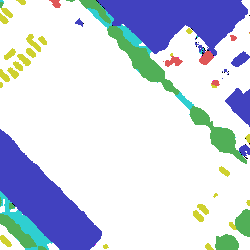
\includegraphics[width=\textwidth]{ndsm_fail_fusenet}
        \caption{V-FuseNet}
    \end{subfigure}
	\caption{Les erreurs dans le \glsname{MNH} du jeu de données \glsname{ISPRS} Vaihingen sont mal gérées par les deux méthodes de fusion. Ici, un bâtiment entier disparaît.}
    \label{fig:ndsm_fail}
\end{figure}

Si ces architectures multi-modales permettent de bénéficier de données géoréférencées recalées hétérogènes, elles introduisent néanmoins une limitation additionnelle. En effet, bien que les données \gls{Lidar} du jeu de données \gls{ISPRS} soient très denses, la normalisation du modèle de terrain est imparfaite et quelques artefacts ont été générés. Comme signalé par~\citet{marmanis_classification_2017}, plusieurs bâtiments sont absents du \gls{MNH}, une hauteur de \SI{0}{\meter} ayant été attribuée aux pixels correspondants. Cela cause des problèmes significatifs de classification pour les deux méthodes de fusion, comme illustré par la~\cref{fig:ndsm_fail}. La solution proposée par~\cite{marmanis_classification_2017} consiste à manuellement corriger le \gls{MNH}, mais cette méthode ne passe pas à l'échelle. Des stratégies robustes à la perte d'une modalité ou aux données bruitées pourraient permettre de résoudre ce problème, en utilisant par exemple les \emph{hallucination networks} de~\citet{hoffman_learning_2016} pour inférer les données manquantes~\cite{kampffmeyer_semantic_2016}. Les travaux récents sur les modèles génératifs pourraient également permettre de diminuer le sur-apprentissage et améliorer la robustesse des modèles en entraînant ceux-ci sur des données synthétiques bruitées~\cite{xie_adversarial_2017}.

%Due to limitations and noise in the Lidar point cloud, such as missing or aberrant points, the DSM and subsequently the nDSM present some artifacts. As reported in~\cite{marmanis_classification_2016}, some buildings vanish in the nDSM and the relevant pixels are falsely attributed a height of 0. This causes significant misclassification in the composite image that are poorly handled by both fusion methods, as illustrated in~\cref{fig:ndsm_fail}. \cite{marmanis_classification_2016} worked around this problem by manually correcting the nDSM, though this method does not scale to bigger datasets. Therefore, improving the method to be robust to impure data and artifacts could be helpful, e.g. by using hallucination networks~\cite{hoffman_learning_2016} to infer the missing modality as proposed in~\cite{kampffmeyer_semantic_2016}. We think that the V-FuseNet architecture could be adapted for such a purpose by using the virtual branch to encode missing data. Moreover, recent work on generative models might help alleviate overfitting and improve robustness by training on synthetic data, as proposed in~\cite{Xie_2017_ICCV}.


\section{Connaissances \textit{a priori}}

\subsection{OpenStreetMap}

\glsfirst{OSM} est un \gls{SIG} libre et participatif alimenté par un ensemble de contributeurs bénévoles qui cartographient les lieux qui leur sont familiers. Les contributeurs peuvent utiliser l'éditeur en ligne pour annoter des fonds de carte géoréférencés en y ajoutant ou en mettant à jour les éléments du réseau routier, les empreintes au sol des bâtiments, les espaces verts, etc. En plus de ces éditions manuelles, la communauté \gls{OSM} utilise certaines sources de données officielles, comme le cadastre de l'État français afin de mettre à jour les limites administratives des entités géographiques ou pour importer les nouveaux bâtis. Le principal intérêt d'\gls{OSM} est qu'il s'agit de la plus grande base de données d'information géographique sous licence libre au monde. La base de données contient des informations sur une large taxonomie d'entités géographiques, allant des autoroutes aux parcs de loisir en passant par les églises, les cimetières ou les parcelles agricoles.

Peu de travaux se sont penchés sur l'intégration des données \gls{OSM} pour l'apprentissage automatique depuis l'ouverture du site en 2004. Le plus souvent, \gls{OSM} est utilisée comme vérité terrain pour la détection de routes et de bâtiments~\cite{mnih_machine_2013,maggiori_learning_2017} dans un contexte d'apprentissage supervisé ou pour le recalage automatique d'images satellites~\cite{vakalopoulou_simultaneous_2016}. \citet{isola_image--image_2016} se sont intéressés à la génération automatique de tuiles \gls{OSM} à partir d'images satellites, mais seulement à des fins visuelles, sans évaluation selon des métriques de classification. Pourtant, \gls{OSM} est une source de données riche permettant d'extraire de l'information géographique sémantique de haut niveau.
\citet{chen_deepvgi_2017} ont de fait utilisé des méthodes d'apprentissage actif pour détecter automatiquement les objets non encore présents dans \gls{OSM} afin de les suggérer aux contributeurs. \citet{danylo_contributing_2016} ont utilisé des forêts aléatoires appliquées sur certaines couches de données \gls{OSM} pour prédire des zones climatologiques locales, tandis que \citet{geis_joint_2017} se sont penchés sur la détection automatique de zones sujettes à des catastrophes naturelles.

Ici, nous suggérons d'utiliser les couches sémantiques d'\gls{OSM} comme entrée à un réseau de neurones profond pour la cartographie automatisée. L'idée est d'exploiter la donnée sémantique, possiblement bruitée et incomplète d'\gls{OSM} afin d'extraire de l'information plus riche à une résolution supérieure. En effet, cette approche est nouvelle et dépasse le cadre habituel de transformation image $\rightarrow$ \gls{OSM}. À l'inverse, il s'agit d'exploiter et d'enrichir les multiples sources d'information existantes, qu'elles soient sous forme d'images ou de \glspl{SIG}.

Pour ce faire, nous considérons le jeu de données \gls{ISPRS} Potsdam sur lequel nous récupérons les données \gls{OSM} de 2017. Nous sélectionnons les couches correspondant aux routes, aux empreintes de bâtiments, aux zones d'eau et aux espaces verts. Les routes sont définies dans \gls{OSM} comme une collection d'éléments linéaires. Par conséquent, en fonction du type de route indiqué dans \gls{OSM}, nous assignons une largeur arbitraire à celles-ci. En outre, les bâtiments, espaces verts et zones d'eau ne correspondent pas nécessairement entièrement aux images aériennes du jeu de données, soit à cause de constructions nouvelles (les images ont été acquises en 2014) , soit car les annotations \gls{OSM} sont incomplètes par endroit. Nous générons ainsi un raster à la même résolution que les images \gls{RVB} contenant 4 canaux binaires\,: un pour le masque des routes, un pour les bâtiments, un pour l'eau et un pour les espaces verts.

\begin{figure}[h]
  \foreach\picname\picpath in {Image \glssymbol{RVB}/potsdam_rgb_4_12,Tuile \glsname{OSM}/potsdam_osmtile_4_12,Raster \glsname{OSM}/potsdam_osm_4_12,Vérité terrain/potsdam_gt_4_12}{%
  \begin{subfigure}{0.25\textwidth}
    \includegraphics[width=\textwidth]{\picpath}
    \caption*{\picname}
  \end{subfigure}%
  }%
  \caption[Tuile 4\_12 du jeu de données \glsname{ISPRS} Potsdam et données \glsname{OSM} correspondantes.]{Tuile 4\_12 du jeu de données \glsname{ISPRS} Potsdam et données \glsname{OSM} correspondantes.\\
  \isprslegende
  }
  \label{fig:dataset_potsdam}
\end{figure}

\subsection{Information \textit{a priori} comme capteur virtuel}

L'idée de notre approche est de traiter le raster \gls{OSM} ainsi formé comme un capteur virtuel, c'est-à-dire comme une source de données complémentaire aux images optiques. Le raster ainsi formé contient une information partielle et incomplète, mais pouvant néanmoins faciliter le travail du réseau profond. En effet, plutôt que d'apprendre à reconnaître un bâtiment uniquement à partir de l'image optique, un réseau muni des deux sources de données peut se reposer en partie sur les annotations \gls{OSM} pour repérer les bâtiments, et consacrer une partie de ses poids à gérer d'autres cas de figure plus difficiles. Plutôt que de réinventer entièrement la carte, le modèle peut donc incrémentalement venir enrichir l'information géographique pré-existante à partir de la donnée optique, en contraste avec les approches traditionnelles.

Nous appliquons donc les méthodes de fusion de donnée FuseNet et de correction résiduelle en utilisant comme entrées les images optiques et les couches \gls{OSM}.

Lorsque les classes d'intérêt de la segmentation sémantique sont déjà présentes dans les données \gls{OSM}, comme pour les bâtiments ou les routes, il est possible de les utiliser comme premières approximations de la vérité terrain. Celles-ci pourront ensuite être raffinées pour corriger les imprécisions de \gls{OSM} et prédire les classes manquantes. Ce procédé s'apparente ainsi à l'apprentissage par résidu~\cite{he_deep_2016} et à l'apprentissage par raffinement~\cite{lin_refinenet_2016}, tous deux connus pour améliorer les performances des \glspl{CNN} et \glspl{FCN}.

Ici, nous utilisons un simple \gls{FCN} composé du premier bloc convolutif de VGG-16~\cite{simonyan_very_2014}, afin de convertir les données raster \gls{OSM} en cartes sémantiques approchant la vérité terrain. Ce modèle sera noté OSMNet par la suite. Les données optiques sont traitées par un \gls{FCN} dérivé du modèle SegNet~\cite{badrinarayanan_segnet_2017} en suivant l'approche de~\cite{audebert_semantic_2016}. SegNet est un réseau de neurones encodeur-décodeur modélisant la projection d'une image dans un espace de cartes sémantiques à la même résolution. En utilisant ces deux modèles, nous pouvons alors calculer une carte de prédiction moyenne combinant les deux sources d'entrée. Dans ce cas, si $\mathcal{I}$ constitue l'image d'entrée, $\mathcal{O}$ la donnée \gls{OSM}, $P_{opt}$ la fonction de prédiction de SegNet et $P_{osm}$ la fonction de prédiction de OSMNet, la prédiction finale $P$ se calcule par :
%In our case, we can use a simple FCN with only two layers to convert the raw rasterized OSM data into a semantic map that approximates the ground truth, trained with the usual backpropagation technique. This FCN will be denoted OSMNet in the following sections. The optical data will then be used as input to a FCN model to infer a semantic segmentation that will complete the approximate map derived from OSM. In this work, we will use the SegNet architecture~\cite{badrinarayanan_segnet_2015} that we will train following the guidelines from~\cite{audebert_semantic_2016}. SegNet is an encoder-decoder deep neural network that projects an input image into a semantic map with the same resolution. Using these two models, we can compute the average prediction computed using the two data sources. In this framework, if we denote $I$ the input image, $O$ the input OSM raster, $P_{opt}$ the prediction function for SegNet and $P_{osm}$ the prediction function for OSMNet, the final prediction $P$ is:
\begin{equation}
P(\mathcal{I}, \mathcal{O}) = \frac{1}{2} (P_{opt}(\mathcal{I}) + P_{osm}(\mathcal{O}))~.
\end{equation}

%If $P_{osm}(O)$ is already an adequate approximation of the ground truth $GT$, then the training process will try to minimize:
Si $P_{osm}(\mathcal{O})$ est une bonne approximation de la vérité terrain $VT$, alors la phase d'optimisation minimise~:
\begin{equation}
P_{opt}(\mathcal{I}) \propto VT - P_{osm}(\mathcal{O}) \ll VT~,
\end{equation}
%which should have a similar effect on the training process than the residual learning from~\cite{he_deep_2016}.
ce qui est similaire à l'apprentissage par résidu~\cite{he_deep_2016}.

En outre, pour raffiner encore cette prédiction moyenne, nous utilisons la correction résiduelle (CR)~\cite{audebert_semantic_2016}. Ce réseau de neurones est un \gls{FCN} constitué d'un unique bloc convolutif classique permettant d'apprendre la correction à appliquer à la prédiction moyenne, cette fois-ci pondérée par classe, pour exploiter la complémentarité des données \gls{OSM} et optiques. En notant $C$ la fonction de prédiction du module de correction résiduelle, en vertu de l'\cref{eq:residual_correction}~:
%Moreover, to refine even further this average map, we use a residual correction network~\cite{audebert_semantic_2016}. This module consists in a residual three-layer FCN that learns how to correct the average prediction using the complementary information from the OSM and optical data sources. If we denote $C$ the prediction function of the residual correction network, we finally have:
\begin{equation}
P(\mathcal{I}, \mathcal{O}) = \frac{1}{2} (P_{opt}(\mathcal{I}) + P_{osm}(\mathcal{O})) + C(Z_{opt}(\mathcal{I}), Z_{osm}(\mathcal{O}))~,
\end{equation}
où $Z_{opt}$ et $Z_{osm}$ sont les cartes d'activation finales de SegNet et OSMNet, respectivement.
%where $Z_{opt}$ and $Z_{osm}$ are the last feature maps from SegNet and OSMNet, respectively.

\begin{figure}[h]
  \resizebox{\textwidth}{!}{\documentclass{standalone}
\usepackage{tikz}
\usepackage{ifthen}
%%%%%%%%%%%%%%%%%%%%%%%%%%%%%%%%%%%%%%%%
%           Commandes perso            %
%%%%%%%%%%%%%%%%%%%%%%%%%%%%%%%%%%%%%%%%

%% Figures centrées, et en position 'here, top, bottom or page'
\newenvironment{figureth}{%
		\begin{figure}[htbp]
			\centering
	}{
		\end{figure}
		}


%% Tableaux centrés, et en position 'here, top, bottom or page'
\newenvironment{tableth}{%
		\begin{table}[htbp]
			\centering
			%\rowcolors{1}{coleurtableau}{coleurtableau}
	}{
		\end{table}
		}

%% Sous-figures centrées, en position 'top'
\newenvironment{subfigureth}[1]{%
	\begin{subfigure}[t]{#1}
	\centering
}{
	\end{subfigure}
}

\newcommand{\citationChap}[2]{%
	\epigraph{\og \textit{#1} \fg{}}{#2}
}

%% On commence par une page impaire quand on change le style de numérotation de pages
\let\oldpagenumbering\pagenumbering
\renewcommand{\pagenumbering}[1]{%
	\cleardoublepage
	\oldpagenumbering{#1}
}

%% Légende du dataset ISPRS
\newcommand\isprslegende{
Légende\,: \textcolor{Black}{blanc}\,: routes, \textcolor{Blue}{bleu}\,: bâtiments, \textcolor{Cerulean}{cyan}\,: végétation basse, \textcolor{OliveGreen}{vert}\,: arbres, \textcolor{Dandelion}{jaune}\,: véhicules, \textcolor{BrickRed}{rouge}\,: autre.
}

%% Dessiner des réseaux de neurones avec Tikz
\newcommand{\convlayer}[9]{%{h}{w}{d}{name}{color}{x}{y}{z}%{note w}{note h}{note d}
   \def\h{#1}
   \def\w{#2}
   \def\d{#3}
   \def\name{#4}
   \ifthenelse {\equal{#5} {}} {\def\col{white}} {\def\col{#5}}
   \def\x{#6}
   \ifthenelse {\equal{#7} {}} {\def\y{0}} {\def\y{#7}}
   \ifthenelse {\equal{#8} {}} {\def\z{0}} {\def\z{#8}}
   % ne faites pas ça chez vous !
   \ifthenelse {\equal{#9} {}} {\convlayercontinued{}{}{}} {\convlayercontinued#9}
}

\newcommand\convlayercontinued[3]{
   \def\notew{#1}
   \def\noteh{#2}
   \def\noted{#3}
   \coordinate (A) at (\x-\d/2,  \y-\h/2, \z-\w/2);
   \coordinate (B) at (\x-\d/2,  \y-\h/2, \z+\w/2);
   \coordinate (C) at (\x-\d/2,  \y+\h/2, \z+\w/2);
   \coordinate (D) at (\x-\d/2,  \y+\h/2, \z-\w/2);
   \coordinate (E) at (\x+\d/2,  \y-\h/2, \z-\w/2);
   \coordinate (F) at (\x+\d/2,  \y-\h/2, \z+\w/2);
   \coordinate (G) at (\x+\d/2,  \y+\h/2, \z+\w/2);
   \coordinate (H) at (\x+\d/2,  \y+\h/2, \z-\w/2);

    \draw [draw opacity=0.3, fill opacity=0.8, fill=\col!60!white] (A) -- (B) -- (C) -- (D) -- cycle;
    \draw [draw opacity=0.3, fill opacity=0.8, fill=\col!60!white] (A) -- (B) -- (F) -- (E) -- cycle;
    % Face haut
    %\draw [left color=\col!60!white, right color=\col!80!white, shading=axis, shading angle=180] (C) -- (D)  -- (H) -- (G) -- cycle;
    \draw [fill opacity=0.9, fill=\col!70!white] (C) -- node[rotate=45,above] {\small \name} (D) -- (H) -- (G) -- cycle;
    %\draw [fill opacity=0.9, fill=\col!70!white] (C) -- (D) -- node[above] {\small \name} (H) -- (G) -- cycle;
    % Face droite
    \draw [fill opacity=0.9, fill=\col!60!white] (E) -- node[pos=0.75,rotate=45,below] {\scriptsize \notew} (F) -- (G) --  (H) -- cycle;
    % Face avant
    %\draw [shading=axis, left color=\col!60!white, right color=\col!40!white, shading angle=-45] (B) -- node[above,rotate=90] {\scriptsize \noteh} (C) -- (G) -- (F) -- node[below] {\scriptsize \noted}  cycle;
    \draw [fill opacity=0.9, fill=\col!50!white] (B) -- node[above,rotate=90] {\scriptsize \noteh} (C) -- (G) -- (F) -- node[below] {\scriptsize \noted}  cycle;
}

\newcommand{\fclayer}[8]{%{h}{w}{name}{color}{x}{y}{z}
   \def\h{#1}
   \def\w{#2}
   \def\name{#3}
   \ifthenelse {\equal{#4} {}} {\def\col{white}} {\def\col{#4}}
   \def\x{#5}
   \def\y{#6}
   \def\z{#7}
   \def\note{#8}
   \coordinate (A) at (\x-\w/2,  \y-\h/2, \z);
   \coordinate (B) at (\x+\w/2,  \y-\h/2, \z);
   \coordinate (C) at (\x+\w/2,  \y+\h/2, \z);
   \coordinate (D) at (\x-\w/2,  \y+\h/2, \z);

   \pgfmathparse{4*\w}\let\boxwidth\pgfmathresult
    \draw [fill=\col] (A) -- node[below,text width=\boxwidth cm,align=center] {\scriptsize \note} (B) -- (C) -- (D) -- cycle;

    \node (N) at ($(A)!0.5!(B)+(0,-1,0)$) {\name};
}

\newcommand{\alexnet}[4]{%{scale}{x}{y}{z}
  \def\scale{#1}
  \def\alexx{#2}
  \def\alexy{#3}
  \def\alexz{#4}


  \def\coblue{blue!50!white}
  \def\fcgrey{gray!50!white}

  \convlayer{1.3*\scale}{1.3*\scale}{0.02*\scale}{Image}{\coblue}{\alexx}{\alexy}{\alexz}{{227}{227}{3}}
  \convlayer{1.1*\scale}{1.1*\scale}{0.08*\scale}{Conv1}{\coblue}{\alexx+0.7*\scale}{\alexy}{\alexz}{{55}{55}{96}}
  \convlayer{0.7*\scale}{0.7*\scale}{0.5*\scale}{Conv2}{\coblue}{\alexx+1.5*\scale}{\alexy}{\alexz}{{27}{27}{256}}
  \convlayer{0.5*\scale}{0.5*\scale}{0.8*\scale}{Conv3}{\coblue}{\alexx+2.6*\scale}{\alexy}{\alexz}{{13}{13}{384}}
  \convlayer{0.5*\scale}{0.5*\scale}{0.8*\scale}{Conv4}{\coblue}{\alexx+3.8*\scale}{\alexy}{\alexz}{{13}{13}{384}}
  \convlayer{0.5*\scale}{0.5*\scale}{0.5*\scale}{Conv5}{\coblue}{\alexx+4.8*\scale}{\alexy}{\alexz}{{13}{13}{256}}
  \fclayer{\scale}{0.1*\scale}{FC1}{\fcgrey}{\alexx+5.4*\scale}{\alexy}{\alexz}{4096}
  \fclayer{\scale}{0.1*\scale}{FC2}{\fcgrey}{\alexx+5.7*\scale}{\alexy}{\alexz}{4096}
  \fclayer{\scale}{0.1*\scale}{FC3}{\fcgrey}{\alexx+6.0*\scale}{\alexy}{\alexz}{1000}
}

\newcommand{\imagelayer}[7]{%{width}{x}{y}{z}{path}{text_up}{text_down}
    \pgfmathparse{#1}\let\w\pgfmathresult
    \begin{scope}[canvas is yz plane at x=#2]
     \node[transform shape] (source) at (#3, #4) {\includegraphics[angle=-90,width=\w cm]{#5}};
    \end{scope}
     \node [transform shape, rotate=45, above] at (source.east) {#6};
     \node [transform shape, rotate=45, below] at (source.west) {\scriptsize{#7}};
}

\def\fourier{\mathcal{F}}

\newcommand{\lightspectrum}{%
\pgfplotsset{
    % this *defines* a custom colormap ...
    colormap={slategraywhite}{color(0cm)=(red); color(1cm)=(red); color(2cm)=(red); color(3cm)=(red); color(4cm)=(orange); color(5cm)=(yellow); color(6cm)=(green); color(7cm)=(blue); color(8cm)=(blue); color(9cm)=(purple); color(10cm)=(purple); color(12cm)=(black)}
}
\node at (1.5, 2.7) {\small 1mm};
\node at (4, 3) {Infrarouge};
\node at (7.75, 2.7) {\small 800nm};
\node at (9, 3) {Visible};
\node at (10.5, 2.7) {\small 400nm};
\node at (12, 3) {Ultraviolet};
\node at (13.5, 2.7) {\small 10nm};
\draw[->] (1, 2.5) -- (14, 2.5);
\begin{axis}[hide axis,width=16cm,height=4cm,colormap name=slategraywhite]
\addplot[domain=20:1000,samples=1500,ultra thick, point meta=x*x,mesh]{sin(x*x/80)};
\end{axis}
}

% Union généralisée
\newcommand{\wbigcup}{\mathop{\bigcup}\displaylimits}

\newcommand{\res}[2]{#1 {\footnotesize $\pm$ #2}}
\newcommand{\bres}[2]{\textbf{#1} {\footnotesize $\pm$ #2}}
\newcommand{\bbres}[2]{\res{\textit{#1}}{#2}}

\newcommand{\drawkernel}[9]{
\begin{tikzpicture}
	\draw[step=1cm,gray!50!white,very thin] (0,0) grid (3,3);
	\kernelnode{0.5}{0.5}{#1};
	\kernelnode{0.5}{1.5}{#2};
	\kernelnode{0.5}{2.5}{#3};
	\kernelnode{1.5}{0.5}{#4};
	\kernelnode{1.5}{1.5}{#5};
	\kernelnode{1.5}{2.5}{#6};
	\kernelnode{2.5}{0.5}{#7};
	\kernelnode{2.5}{1.5}{#8};
	\kernelnode{2.5}{2.5}{#9};
\end{tikzpicture}
}

\newcommand{\kernelnode}[3]{%{x}{y}{value}
	\ifthenelse{\equal{#3}{0}}{
		\def\kcolor{gray}
	}{
		\def\kcolor{black}
	}
	\node[\kcolor] at (#1, #2) {#3};
}

\newcommand{\chapsummary}[1]{
\section*{Résumé du chapitre :}
\parbox{0.9\linewidth}{
\setlength{\parindent}{4ex}
#1}
}

\newcommand{\eqname}[1]{\tag*{\small (#1)}}

\begin{document}

\begin{tikzpicture}[]
\usetikzlibrary{3d}
\usetikzlibrary{calc}

\def\scale{5}
\def\segx{0}
\def\segy{+0.8*\scale}
\def\segz{0}
\def\depth{0.03*\scale}
\def\size{\scale}

    \begin{scope}[canvas is yz plane at x=-\segx-0.4*\scale]
     \node[transform shape] (source) at (\segy, 0) {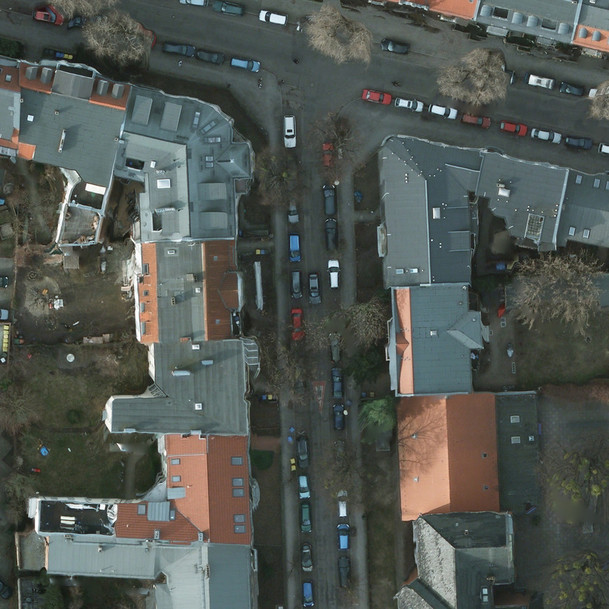
\includegraphics[width=6.3cm]{../Chapitre2/potsdam_sample.jpg}};
     \node [transform shape, rotate=-90, below] at (source.west) {\huge{Optique}};
    \end{scope}

\convlayer{\size}{\size}{\depth}{}{blue}{\segx}{\segy}{\segz}{}
\convlayer{\size}{\size}{\depth}{}{blue}{\segx+\depth}{\segy}{\segz}{}
\convlayer{\size}{\size}{\depth}{}{yellow}{\segx+2*\depth}{\segy}{\segz}{}
\node (pool1) at (\segx+2*\depth, \segy+0.5*\size) {};

\pgfmathsetmacro\segx{\segx+0.3*\scale}
\pgfmathsetmacro\depth{2*\depth}
\pgfmathsetmacro\size{0.75*\size}

\convlayer{\size}{\size}{\depth}{}{blue}{\segx}{\segy}{\segz}{}
\convlayer{\size}{\size}{\depth}{}{blue}{\segx+\depth}{\segy}{\segz}{}
\convlayer{\size}{\size}{\depth}{}{yellow}{\segx+2*\depth}{\segy}{\segz}{}
\node (pool2) at (\segx+2*\depth, \segy+0.5*\size) {};

\pgfmathsetmacro\segx{\segx+0.4*\scale}
\pgfmathsetmacro\depth{1.25*\depth}
\pgfmathsetmacro\size{0.75*\size}

\convlayer{\size}{\size}{\depth}{}{blue}{\segx}{\segy}{\segz}{}
\convlayer{\size}{\size}{\depth}{}{blue}{\segx+\depth}{\segy}{\segz}{}
\convlayer{\size}{\size}{\depth}{}{blue}{\segx+2*\depth}{\segy}{\segz}{}
\convlayer{\size}{\size}{\depth}{}{yellow}{\segx+3*\depth}{\segy}{\segz}{}
\node at (\segx+0.25*\size,\segy-\size) {\huge Encodeur};
\node (pool3) at (\segx+3*\depth, \segy+0.5*\size) {};

\pgfmathsetmacro\segx{\segx+0.5*\scale}
\pgfmathsetmacro\depth{1.25*\depth}
\pgfmathsetmacro\size{0.75*\size}

\convlayer{\size}{\size}{\depth}{}{blue}{\segx}{\segy}{\segz}{}
\convlayer{\size}{\size}{\depth}{}{blue}{\segx+\depth}{\segy}{\segz}{}
\convlayer{\size}{\size}{\depth}{}{blue}{\segx+2*\depth}{\segy}{\segz}{}
\convlayer{\size}{\size}{\depth}{}{yellow}{\segx+3*\depth}{\segy}{\segz}{}
\node (pool4) at (\segx+3*\depth, \segy+0.5*\size) {};

\pgfmathsetmacro\segx{\segx+0.6*\scale}
\pgfmathsetmacro\depth{1.25*\depth}
\pgfmathsetmacro\size{0.75*\size}

\convlayer{\size}{\size}{\depth}{}{blue}{\segx}{\segy}{\segz}{}
\convlayer{\size}{\size}{\depth}{}{blue}{\segx+\depth}{\segy}{\segz}{}
\convlayer{\size}{\size}{\depth}{}{blue}{\segx+2*\depth}{\segy}{\segz}{}
\convlayer{\size}{\size}{\depth}{}{yellow}{\segx+3*\depth}{\segy}{\segz}{}
\node (pool5) at (\segx+3*\depth, \segy+0.5*\size) {};

%%%%% DECODER %%%%%%%%

\pgfmathsetmacro\segx{\segx+0.6*\scale}

\node (unpool5) at (\segx+0.5*\depth, \segy+0.5*\size) {};
\convlayer{\size}{\size}{\depth}{}{red}{\segx}{\segy}{\segz}{}
\convlayer{\size}{\size}{\depth}{}{blue}{\segx+\depth}{\segy}{\segz}{}
\convlayer{\size}{\size}{\depth}{}{blue}{\segx+2*\depth}{\segy}{\segz}{}
\convlayer{\size}{\size}{\depth}{}{blue}{\segx+3*\depth}{\segy}{\segz}{}

\pgfmathsetmacro\segx{\segx+0.6*\scale}
\pgfmathsetmacro\depth{0.8*\depth}
\pgfmathsetmacro\size{1.33*\size}

\node (unpool4) at (\segx+0.5*\depth, \segy+0.5*\size) {};
\convlayer{\size}{\size}{\depth}{}{red}{\segx}{\segy}{\segz}{}
\convlayer{\size}{\size}{\depth}{}{blue}{\segx+\depth}{\segy}{\segz}{}
\convlayer{\size}{\size}{\depth}{}{blue}{\segx+2*\depth}{\segy}{\segz}{}
\convlayer{\size}{\size}{\depth}{}{blue}{\segx+3*\depth}{\segy}{\segz}{}

\pgfmathsetmacro\segx{\segx+0.5*\scale}
\pgfmathsetmacro\depth{0.8*\depth}
\pgfmathsetmacro\size{1.33*\size}

\node (unpool3) at (\segx+0.5*\depth, \segy+0.5*\size) {};
\convlayer{\size}{\size}{\depth}{}{red}{\segx}{\segy}{\segz}{}
\convlayer{\size}{\size}{\depth}{}{blue}{\segx+\depth}{\segy}{\segz}{}
\convlayer{\size}{\size}{\depth}{}{blue}{\segx+2*\depth}{\segy}{\segz}{}
\convlayer{\size}{\size}{\depth}{}{blue}{\segx+3*\depth}{\segy}{\segz}{}
\node at (\segx-0.25*\size,\segy-\size) {\huge Décodeur};

\pgfmathsetmacro\segx{\segx+0.4*\scale}
\pgfmathsetmacro\depth{0.8*\depth}
\pgfmathsetmacro\size{1.33*\size}

\node (unpool2) at (\segx+0.5*\depth, \segy+0.5*\size) {};
\convlayer{\size}{\size}{\depth}{}{red}{\segx}{\segy}{\segz}{}
\convlayer{\size}{\size}{\depth}{}{blue}{\segx+\depth}{\segy}{\segz}{}
\convlayer{\size}{\size}{\depth}{}{blue}{\segx+2*\depth}{\segy}{\segz}{}

\pgfmathsetmacro\segx{\segx+0.3*\scale}
\pgfmathsetmacro\depth{0.8*\depth}
\pgfmathsetmacro\size{1.33*\size}

\node (unpool1) at (\segx+0.5*\depth, \segy+0.5*\size) {};
\node (o_unpool1) at (\segx+0.5*\depth, \segy-0.56*\size) {};
\convlayer{\size}{\size}{\depth}{}{red}{\segx}{\segy}{\segz}{}
\convlayer{\size}{\size}{\depth}{}{blue}{\segx+\depth}{\segy}{\segz}{}
\convlayer{\size}{\size}{\depth}{}{blue}{\segx+2*\depth}{\segy}{\segz}{}

\pgfmathsetmacro\segx{\segx+0.3*\scale}
\convlayer{\size}{\size}{0.15\scale}{Prédictions}{brown}{\segx}{\segy}{\segz}{}
\node (pred_opt) at (\segx,\segy,\segz) {};

\newcommand\skipconnection[3][]{%{node1}{node2}
    \draw[->, dotted, very thick] (#2) -- ++(0.085*\size, 0.1*\scale) -- node[above] {#1} ($(#3)+(-0.085*\size, 0.1*\scale)$) -- (#3);
}
\skipconnection{pool5}{unpool5}
\skipconnection{pool4}{unpool4}
\skipconnection{pool3}{unpool3}
\skipconnection{pool2}{unpool2}
\skipconnection[indices]{pool1}{unpool1}


\def\segx{0}
\def\segy{-0.8*\scale}
\def\segz{0}
\def\depth{0.10*\scale}
\def\size{\scale}

    \begin{scope}[canvas is yz plane at x=-\segx-0.4*\scale]
     \node[transform shape] (source) at (\segy, 0) {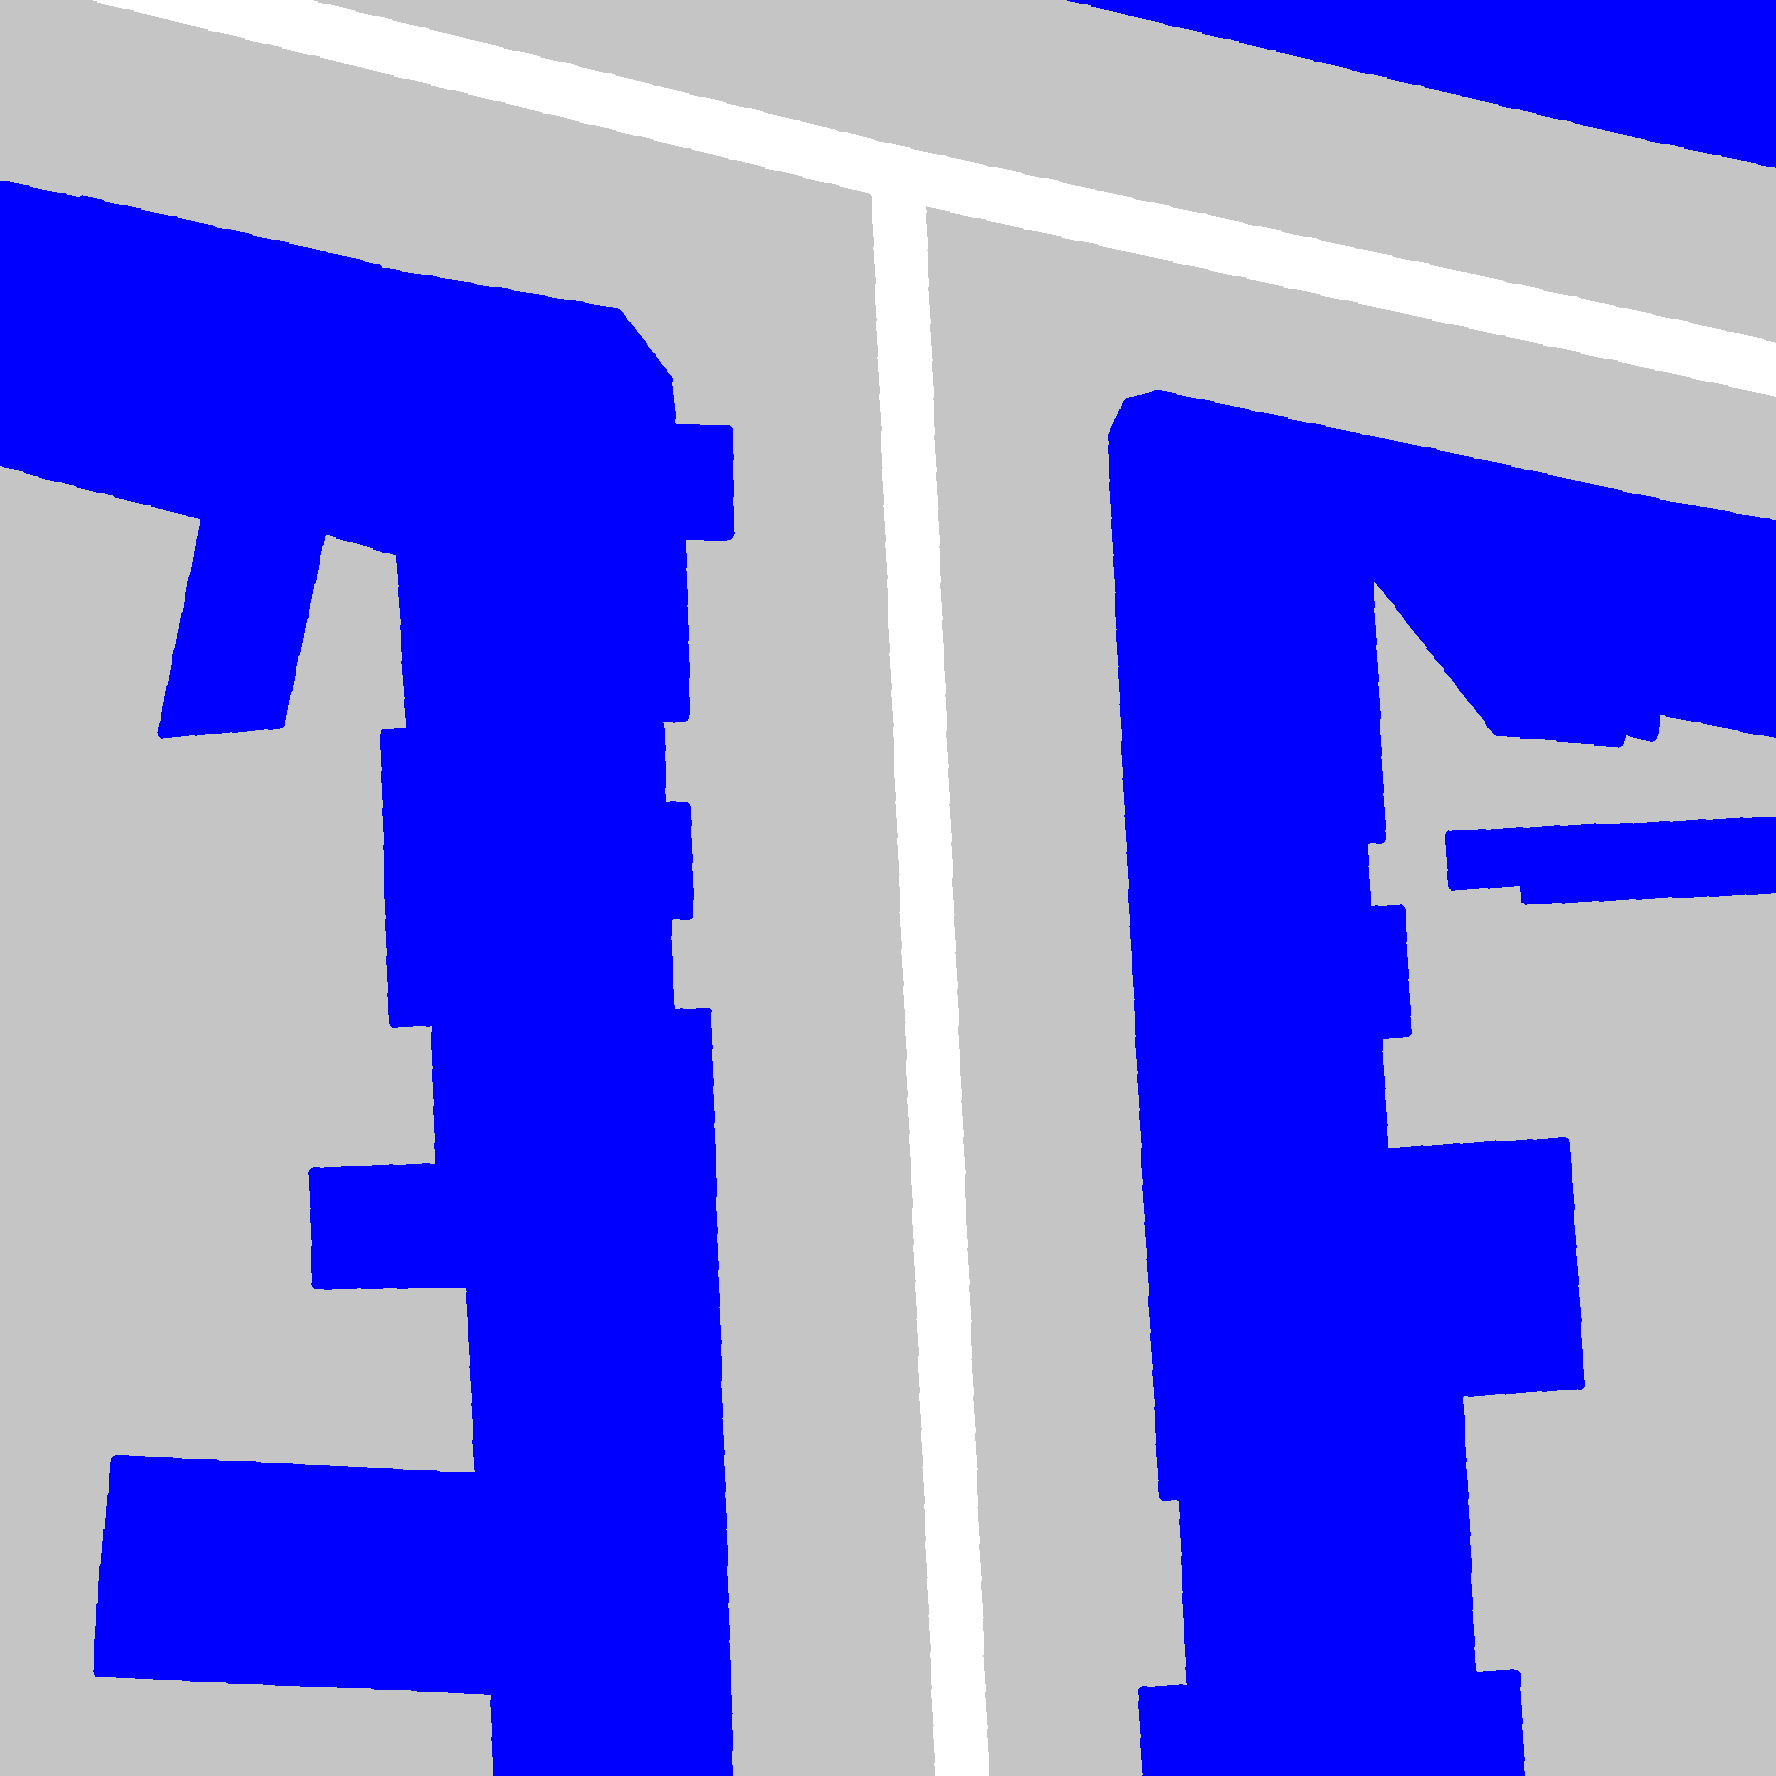
\includegraphics[width=6.3cm]{../Chapitre2/potsdam_sample_osm.png}};
     \node [transform shape, rotate=-90, below] at (source.west) {\huge{OSM}};
    \end{scope}

\convlayer{\size}{\size}{\depth}{}{blue}{\segx}{\segy}{\segz}{}
\convlayer{\size}{\size}{\depth}{}{blue}{\segx+1.5*\depth}{\segy}{\segz}{}
\convlayer{\size}{\size}{\depth}{}{blue}{\segx+3*\depth}{\segy}{\segz}{}
\node (pool1) at (\segx+3.5*\depth, \segy+0.5*\size) {};
\node (c_unpool1) at (\segx+3.5*\depth, \segy+0.5*\size) {};

\pgfmathsetmacro\segx{\segx+0.6*\scale}
\convlayer{\size}{\size}{0.15\scale}{Prédictions}{brown}{\segx}{\segy}{\segz}{}
\node (pred_comp) at (\segx,\segy,\segz) {};

\pgfmathsetmacro\segx{\segx+4.6*\scale}
\def\segy{0}
\def\segz{0}
\def\depth{0.06*\scale}
\def\size{\scale}

\convlayer{\size}{\size}{\depth}{\large concaténation}{cyan}{\segx}{\segy}{\segz}{}
\node (concat) at (\segx-0.01*\size,\segy+0.2*\size,\segz+0.5*\size) {};
\convlayer{\size}{\size}{\depth}{}{blue}{\segx+\depth}{\segy}{\segz}{}
\convlayer{\size}{\size}{\depth}{}{blue}{\segx+2*\depth}{\segy}{\segz}{}
\convlayer{\size}{\size}{\depth}{}{blue}{\segx+3*\depth}{\segy}{\segz}{}

\pgfmathsetmacro\segx{\segx+0.3*\scale}
\convlayer{\size}{\size}{0.15\scale}{}{brown}{\segx}{\segy}{\segz}{}
\node (fus_top) at (\segx, \segy+0.5*\size) {};
\node (fus_bottom) at (\segx, \segy-0.5*\size) {};

\draw[very thick,->] let \p1 = (pred_opt),
              \p2 = (fus_top) in 
          (pred_opt) -- node[above] {$\times 0,5$} (\x2,\y1)  node[yshift=-0.72pt, scale=1.2] {\huge $\bigoplus$}  -- (fus_top);
\draw[very thick,->] let \p1 = (pred_comp),
              \p2 = (fus_bottom) in 
          (pred_comp) -- node[below] {$\times 0,5$} (\x2,\y1) node[scale=1.2,yshift=-0.65pt] {\huge $\bigoplus$} -- (fus_bottom);

\tikzset{
    shadowed/.style={preaction={draw opacity=0.75,transform canvas={shift={(1pt,-1pt)}},draw=gray,very thick}},
  }
\draw[->,ultra thick, looseness=1.07] (o_unpool1) to[out=-90,in=180] node[xshift=0.8cm,above] {caractéristiques} (concat);
\draw[->,ultra thick, looseness=0.5] (c_unpool1) to[out=+90,in=195] (concat);

\pgfmathsetmacro\segx{\segx+0.3*\scale}
\convlayer{\size}{\size}{0.15\scale}{Softmax}{green}{\segx}{\segy}{\segz}{}

\pgfmathsetmacro\segx{\segx+0.35*\scale}
    \begin{scope}[canvas is yz plane at x=\segx]
     \node[transform shape] (output) at (0, 0) {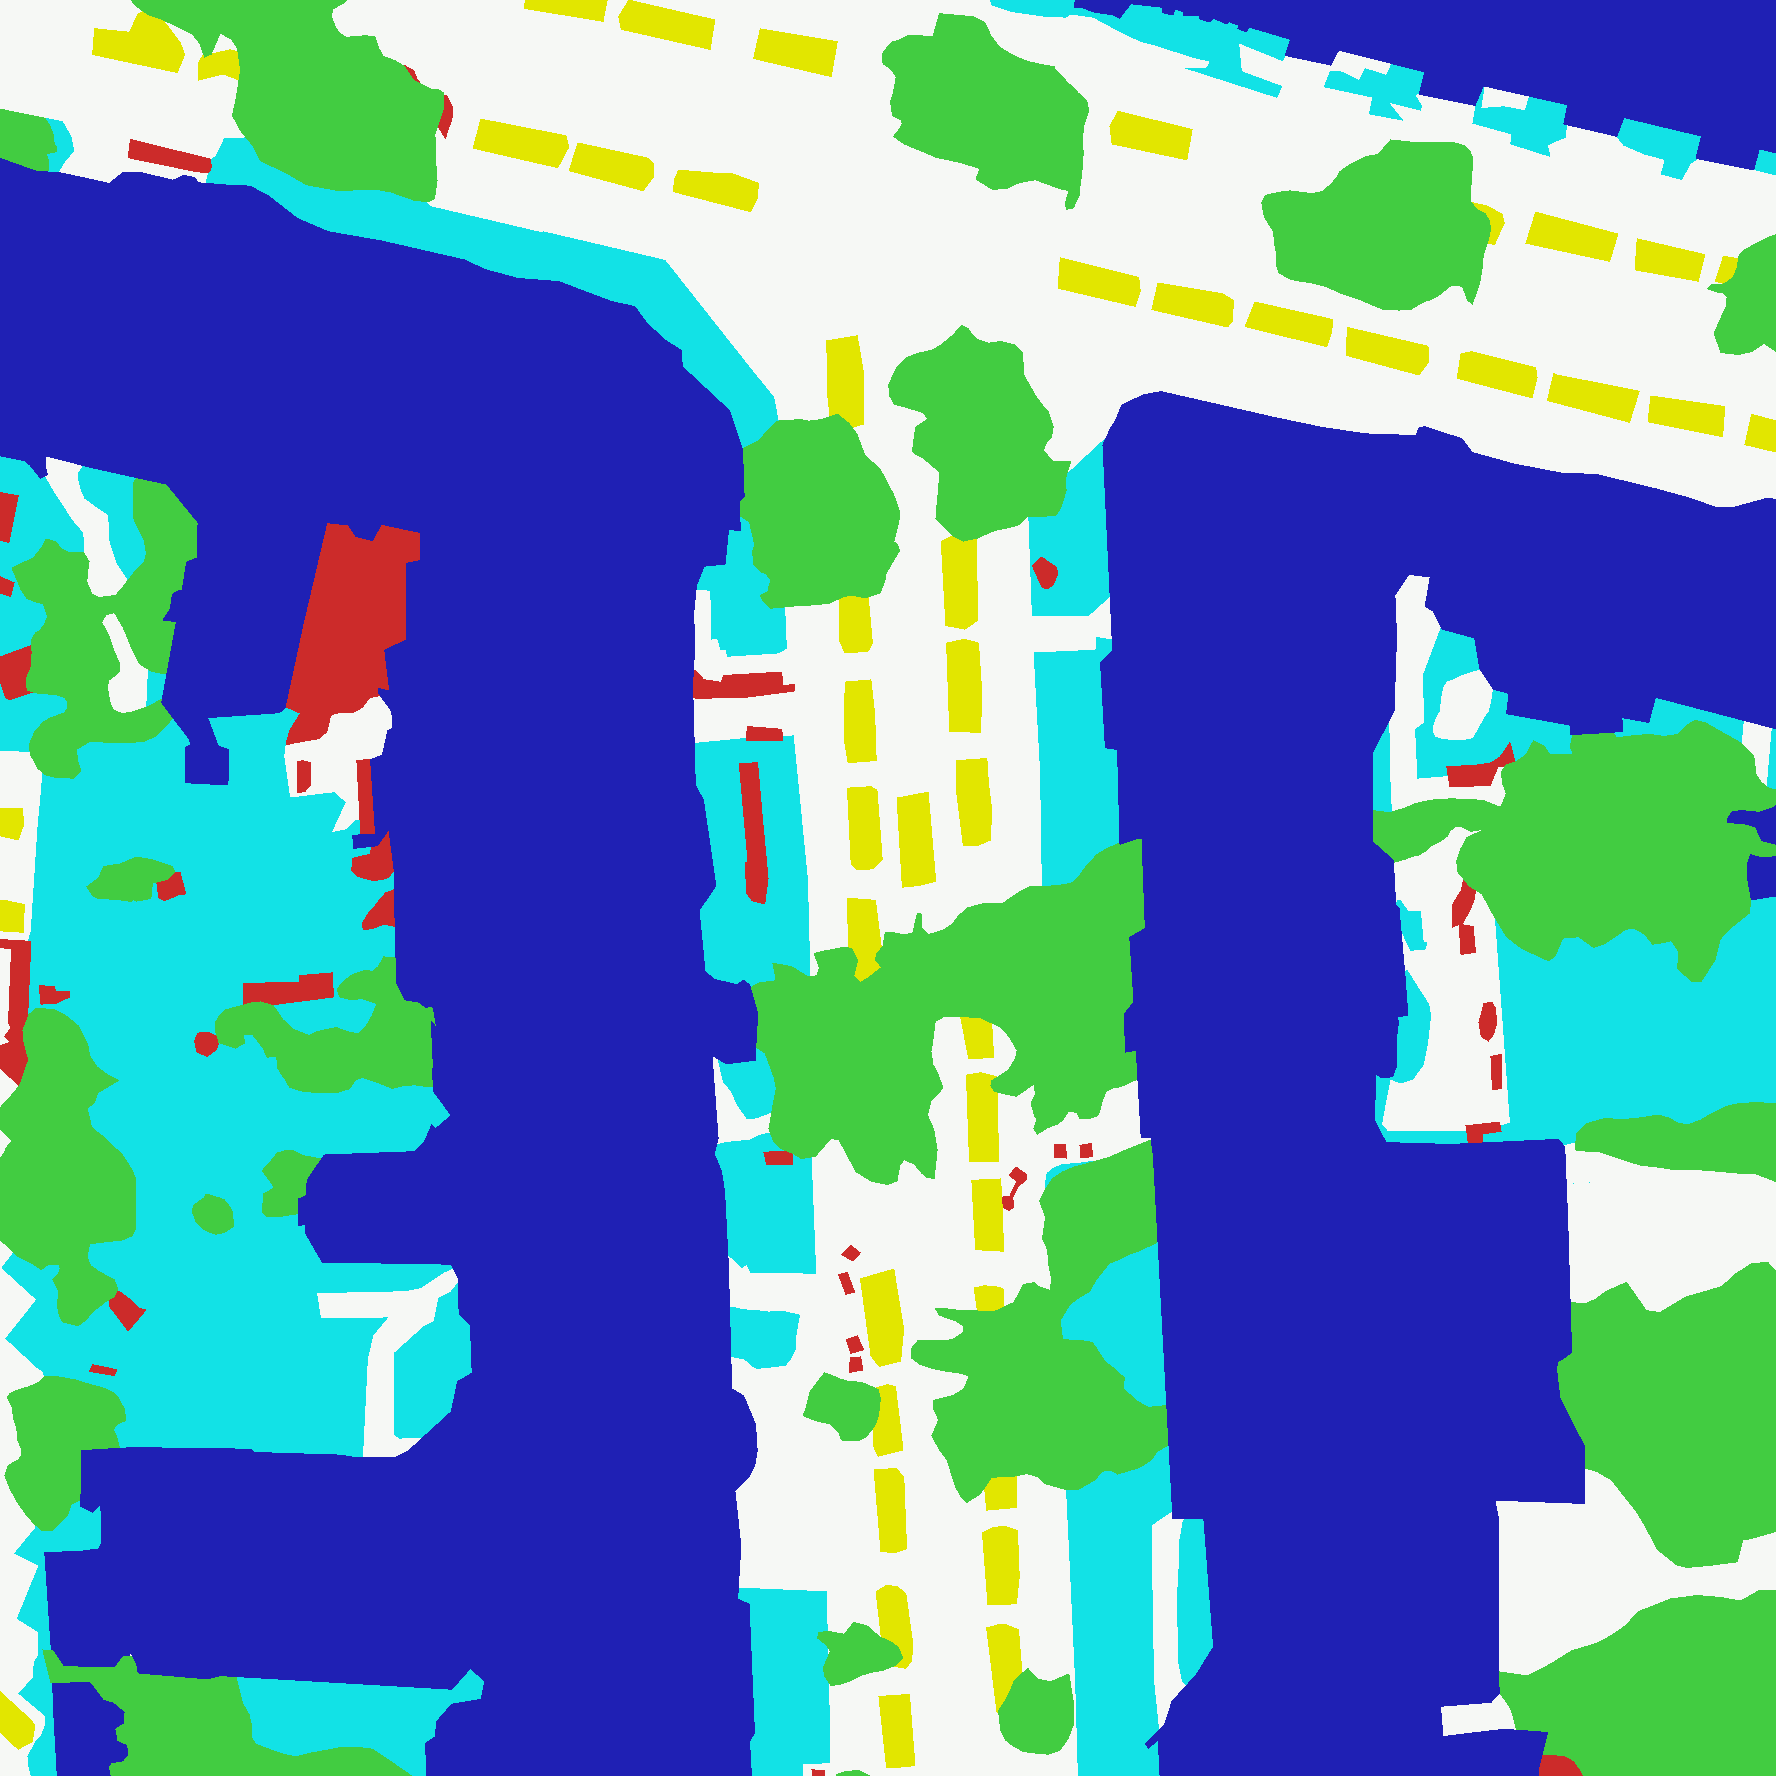
\includegraphics[width=5.5cm]{../Chapitre2/potsdam_sample_gt}};
    \node [transform shape, rotate=-90, below] at (output.west) {\huge{Segmentation}};
    \end{scope}

\newcommand\legendlayer[3]{%{name}{x}{color}
\convlayer{0.1*\scale}{0.1*\scale}{0.2*\scale}{}{#3}{#2}{-1.2*\scale}{0}{}
\node[anchor=west] at (#2+0.125*\scale, -1.2*\scale) {\large = #1};
}
\legendlayer{convolution + BN + ReLU}{1.5*\scale}{blue}
\legendlayer{\emph{maxpooling}}{3*\scale}{yellow}
\legendlayer{\emph{unpooling}}{4*\scale}{red}
\legendlayer{fusion (concaténation)}{5*\scale}{cyan}



\end{tikzpicture}


\end{document}
}
  \caption{Correction résiduelle appliqué à un OSMNet et un SegNet.}
  \label{fig:refinet}
\end{figure}

Dans ce cadre, l'apprentissage par résidu peut être conçu comme la modélisation d'un terme de correction d'erreur, illustré dans la~\cref{fig:refinet}. De cette façon, le raffinement de la carte \gls{OSM} de départ est elle-même raffinée par la correction résiduelle selon un processus itératif à deux étapes.

\subsection{Architectures multi-modales pour l'information géographique}

Les \glspl{FCN} à plusieurs entrées ont été la source de plusieurs études par le passé, notamment dans le cadre du traitement d'images \gls{RGB-D} (ou 2,5D)~\cite{eitel_multimodal_2015}. Dans cet article, nous utilisons l'architecture FuseNet~\cite{hazirbas_fusenet_2016} pour combiner données optiques et \gls{OSM}. FuseNet se réapproprie le modèle SegNet en utilisant non pas un, mais deux encodeurs, un pour chaque source. Après chaque bloc de convolutions, les cartes d'activations neuronales du deuxième encodeur sont sommées aux activations du premier. Cela permet au réseau d'apprendre une représentation conjointe des données exploitant les deux modalités. Un unique décodeur transforme ensuite cette représentation en sur-échantillonnant et en effectuant la classification dans l'espace des classes sémantiques pour chaque pixel. Comme détaillé dans la~\cref{fig:fusenet}, une branche principale apprend la représentation conjointe tandis que la branche auxiliaire n'apprend que les activations liées aux données \gls{OSM}. En notant $P$ la fonction de prédiction de FuseNet, $I$ l'image d'entrée, $O$ la donnée \gls{OSM}, $E_i^{\{opt,osm\}}$ les cartes d'activations après le $i$\textsuperscript{ème} bloc de l'encodeur, $B_i^{\{opt,osm\}}$ les fonctions représentées par le $i$\textsuperscript{ème} bloc de convolutions et $D$ la fonction du décodeur :
\begin{equation}
P(I,O) = D(E_5^{opt}(I,O))
%P(I,O) = D(E(I,O))
\end{equation}
et
\begin{equation}
E_{i+1}^{opt}(I,O) = B_i^{opt}(E_i^{opt}(I, O)) + B_i^{osm}(E_i^{osm}(O))~.
\end{equation}

Nous utilisons le jeu de données \gls{ISPRS} Potsdam sur lequel nous récupérons les données \gls{OSM} correspondantes (cf.~\cref{fig:dataset_potsdam}). Les tuiles étant géo-référencées, nous générons les images \gls{OSM} associées contenant les empreintes de routes, bâtiments, des zones de végétation et de l'eau en utilisant Maperitive\footnote{\url{http://maperitive.net/}}. Les résultats sont obtenus par validation croisée sur 3 partitions du jeu de données.

\subsubsection{Validation expérimentale}
Lors de l'apprentissage, nous extrayons aléatoirement des images de $128\times128$ dans le jeu d'apprentissage, en appliquant des symétries afin d'augmenter le nombre d'exemples. Le réseau est entraîné par descente de gradient en traitant 10 images en parallèle, comme suggéré dans~\cite{audebert_semantic_2016}. Les taux d'apprentissage sont initialisés à 0,005 pour l'encodeur et 0,01 pour le décodeur, puis sont divisés par 2 tous les 30~000 itérations. L'encodeur pour les données \glssymbol{RVB} est initialisé à partir des poids de VGG-16 pré-entraînés sur ImageNet, les autres poids étant initialisés aléatoirement.
%~\cite{he_delving_2015}.
L'évaluation s'effectue via une fenêtre glissante de taille $128\times128$ avec un pas de 64, les prédictions recouvrantes étant moyennées. L'apprentissage prend environ 20 heures sur une carte graphique NVIDIA K20c et l'évaluation moins de 30 minutes. Nous comparons les résultats obtenus avec ceux obtenus par forêt aléatoire (RF) sur l'image pré-segmentée en superpixels. Les caractéristiques utilisées sont les histogrammes de gradients orientés et de couleurs comme descripteur optique, ainsi que l'histogramme des classes \gls{OSM}.
%During training on the \gls{ISPRS} Potsdam dataset, we randomly extract $128\times128$ patches from the training tiles on which we apply random flipping or mirroring as data augmentation. We train a network on a end-to-end fashion, following the guidelines from~\cite{audebert_semantic_2016}, \textit{i.e.} we train a SegNet with a batch size of 10 on the RVB tiles using a Stochastic Gradient Descent (SGD) with a learning rate of 0.01 divided by 10 every 2 epochs ($\simeq$ 30 000 iterations). SegNet's encoder for the RVB data is initialized using VGG-16~\cite{simonyan_very_2014} weights trained on ImageNet, while the decoder is randomly initialized using the MSRA~\cite{he_delving_2015} scheme. The learning rate for the encoder is set to half the learning rate for the decoder. During testing, each tile is processed by sliding a $128\times128$ window with a stride of 64 (\textit{i.e.} 50\% overlap). Multiple predictions for overlapping regions are averaged to smooth the map and reduce visible stitching on the patch borders. Training until convergence ($\simeq$ 150,000 iterations) takes around 20 hours on a NVIDIA K20c, while evaluating on the validation set takes less than 30 minutes.

%On the DFC2017, we re-train SegNet from scratch and the weights are initialized using the MSRA scheme. As the input data has a resolution of 20m/pixel and the output LCZ are expected to be at 100m/pixel resolution, we use a smaller decoder by removing the last three convolutional blocks and the associated pooling layers. The resulting predictions have a resolution of 1:4 the input data and are interpolated to the 100m/pixel resolution. We train the network on randomly flipped $160\times160$ patches with a 50\% overlap. The patches are randomly selected but have to contain at least 5\% of annotated pixels. To avoid learning on non-labeled pixels from the sparse LCZ annotations, we ignore the undefined pixels in the ground truth during loss computation. The network is trained using the Adam~\cite{kingma_adam:_2014} optimizer with a learning rate of 0.01 with a batch size of 10. Training until convergence ($\simeq$ 60,000 iterations) takes around 6 hours on a NVIDIA Titan Pascal, while evaluating on the test set takes less than 5 minutes.

% \begin{figure}
% 	\begin{subfigure}[t]{0.49\linewidth}
%     	\includegraphics[width=\textwidth]{osm_binary}
%         \caption{Binary representation.}
%         \label{fig_osm_modeling_binary}
%     \end{subfigure}
%     \begin{subfigure}[t]{0.49\linewidth}
%     	\includegraphics[width=\textwidth]{osm_dist}
%         \caption{Signed distance transform.}
%         \label{fig_osm_modeling_dist}
%     \end{subfigure}
%     \caption{Representations of the OSM layer for roads.}
%     \label{fig_osm_modeling}
% \end{figure}

% OSM data modelization has to be carefully investigated. Most sensor data is continuous both in the numerical meaning but also in the spatial repartition. In many cases, if the original data is not continuous but sparse, well-chosen representations are used to get the continuity back, \textit{e.g.} the Digital Surface Model which is a continuous topology extracted from the sparse LiDAR point cloud. In our case, the OSM data is sparse and discrete like the labels. Therefore, it is dubious if the deep network will be able to handle all the information using such a representation. We compare two representations, illustrated in~\cref{fig_osm_modeling}:
% \begin{itemize}
% 	\item Sparse tensor representation, which is discrete. For each raster, we have an associated channel in the tensor which is a binary map denoting the presence of the raster class in the specified pixel (cf.~\cref{fig_osm_modeling_binary}).
%     \item Signed distance transform (SDT) representation, which is continuous. We generate for each raster the associated channel corresponding to the distance transform $d$, with $d > 0$ if the pixel is inside the class and $d < 0$ if not (cf.~\cref{fig_osm_modeling_dist}, with a color range from blue to red).
% \end{itemize}

% The signed distance transform was used in~\cite{yuan_automatic_2016} for building extraction in remote sensing data. The continuous representation helped densifying the sparse building footprints that were extracted from a public GIS database and successfully improved the classification accuracy.

\begin{table}[t]
	\caption{Résultats de segmentation sémantique multi-modale avec \glsname{OSM} sur le jeu de données \glsname{ISPRS} Potsdam (scores $F_1$ par classe et pourcentage global de pixels bien classés).}
    \label{table_potsdam_results}
	\begin{tabularx}{\textwidth}{Y c c c c c c c}
    \toprule
    Méthode                 & Route     & Bâtiment& Vég. basse  & Arbre   & Véhicule & Global\\
    \midrule
    RF \gls{IRRVB}          & 77,0\%    & 79,7\%  & 73,1\%      & 59,4\%  & 58,8\%   & 74,2\%\\
    SegNet \gls{RVB}        & 93,0\%    &	92,9\%	&	85,0\%      &	85,1\%  &	95,1\%	 & 89,7\%\\
    \midrule
    RF \gls{IRRVB}+\gls{OSM}& 85,6\%    & 92,4\%  & 73,8\%      & 59,5\%  & 67,6\%   & 80,9\%\\
    CR \gls{RVB}+\gls{OSM}  &	93,9\%    &	92,8\%	&	85,1\%		  &	\textbf{85,2}\%    &	95,8\%	&	90,6\%\\
    FuseNet                 &	\textbf{95,3}\%	&	\textbf{95,9}\%	&	\textbf{86,3}\%	   &	85,1\%	&	\textbf{96,8}\%	&	\textbf{92,3}\%\\
    \bottomrule
    \end{tabularx}
\end{table}

%\paragraph{OSM data representation}
%As can be seen in~\cref{table_potsdam_results}, the signed distance transform (SDT) representation for the OpenStreetMap layers performs slightly worse than its binary counterpart. This might seem counter-intuitive, as the distance transform contains a denser information. However, we suggest that this information might be too diffuse and that the model loses the sharp boundaries and clear transitions of the binary raster on some parts of the dataset. Yet, the difference between the two representations does not impact strongly the final accuracy.

\begin{figure}[h]
\begin{subfigure}{0.33\linewidth}
	\includegraphics[width=\textwidth]{potsdam_rgb_4_12}
    \caption{Image \glssymbol{RVB}}
\end{subfigure}
\hfill
\begin{subfigure}{0.33\linewidth}
    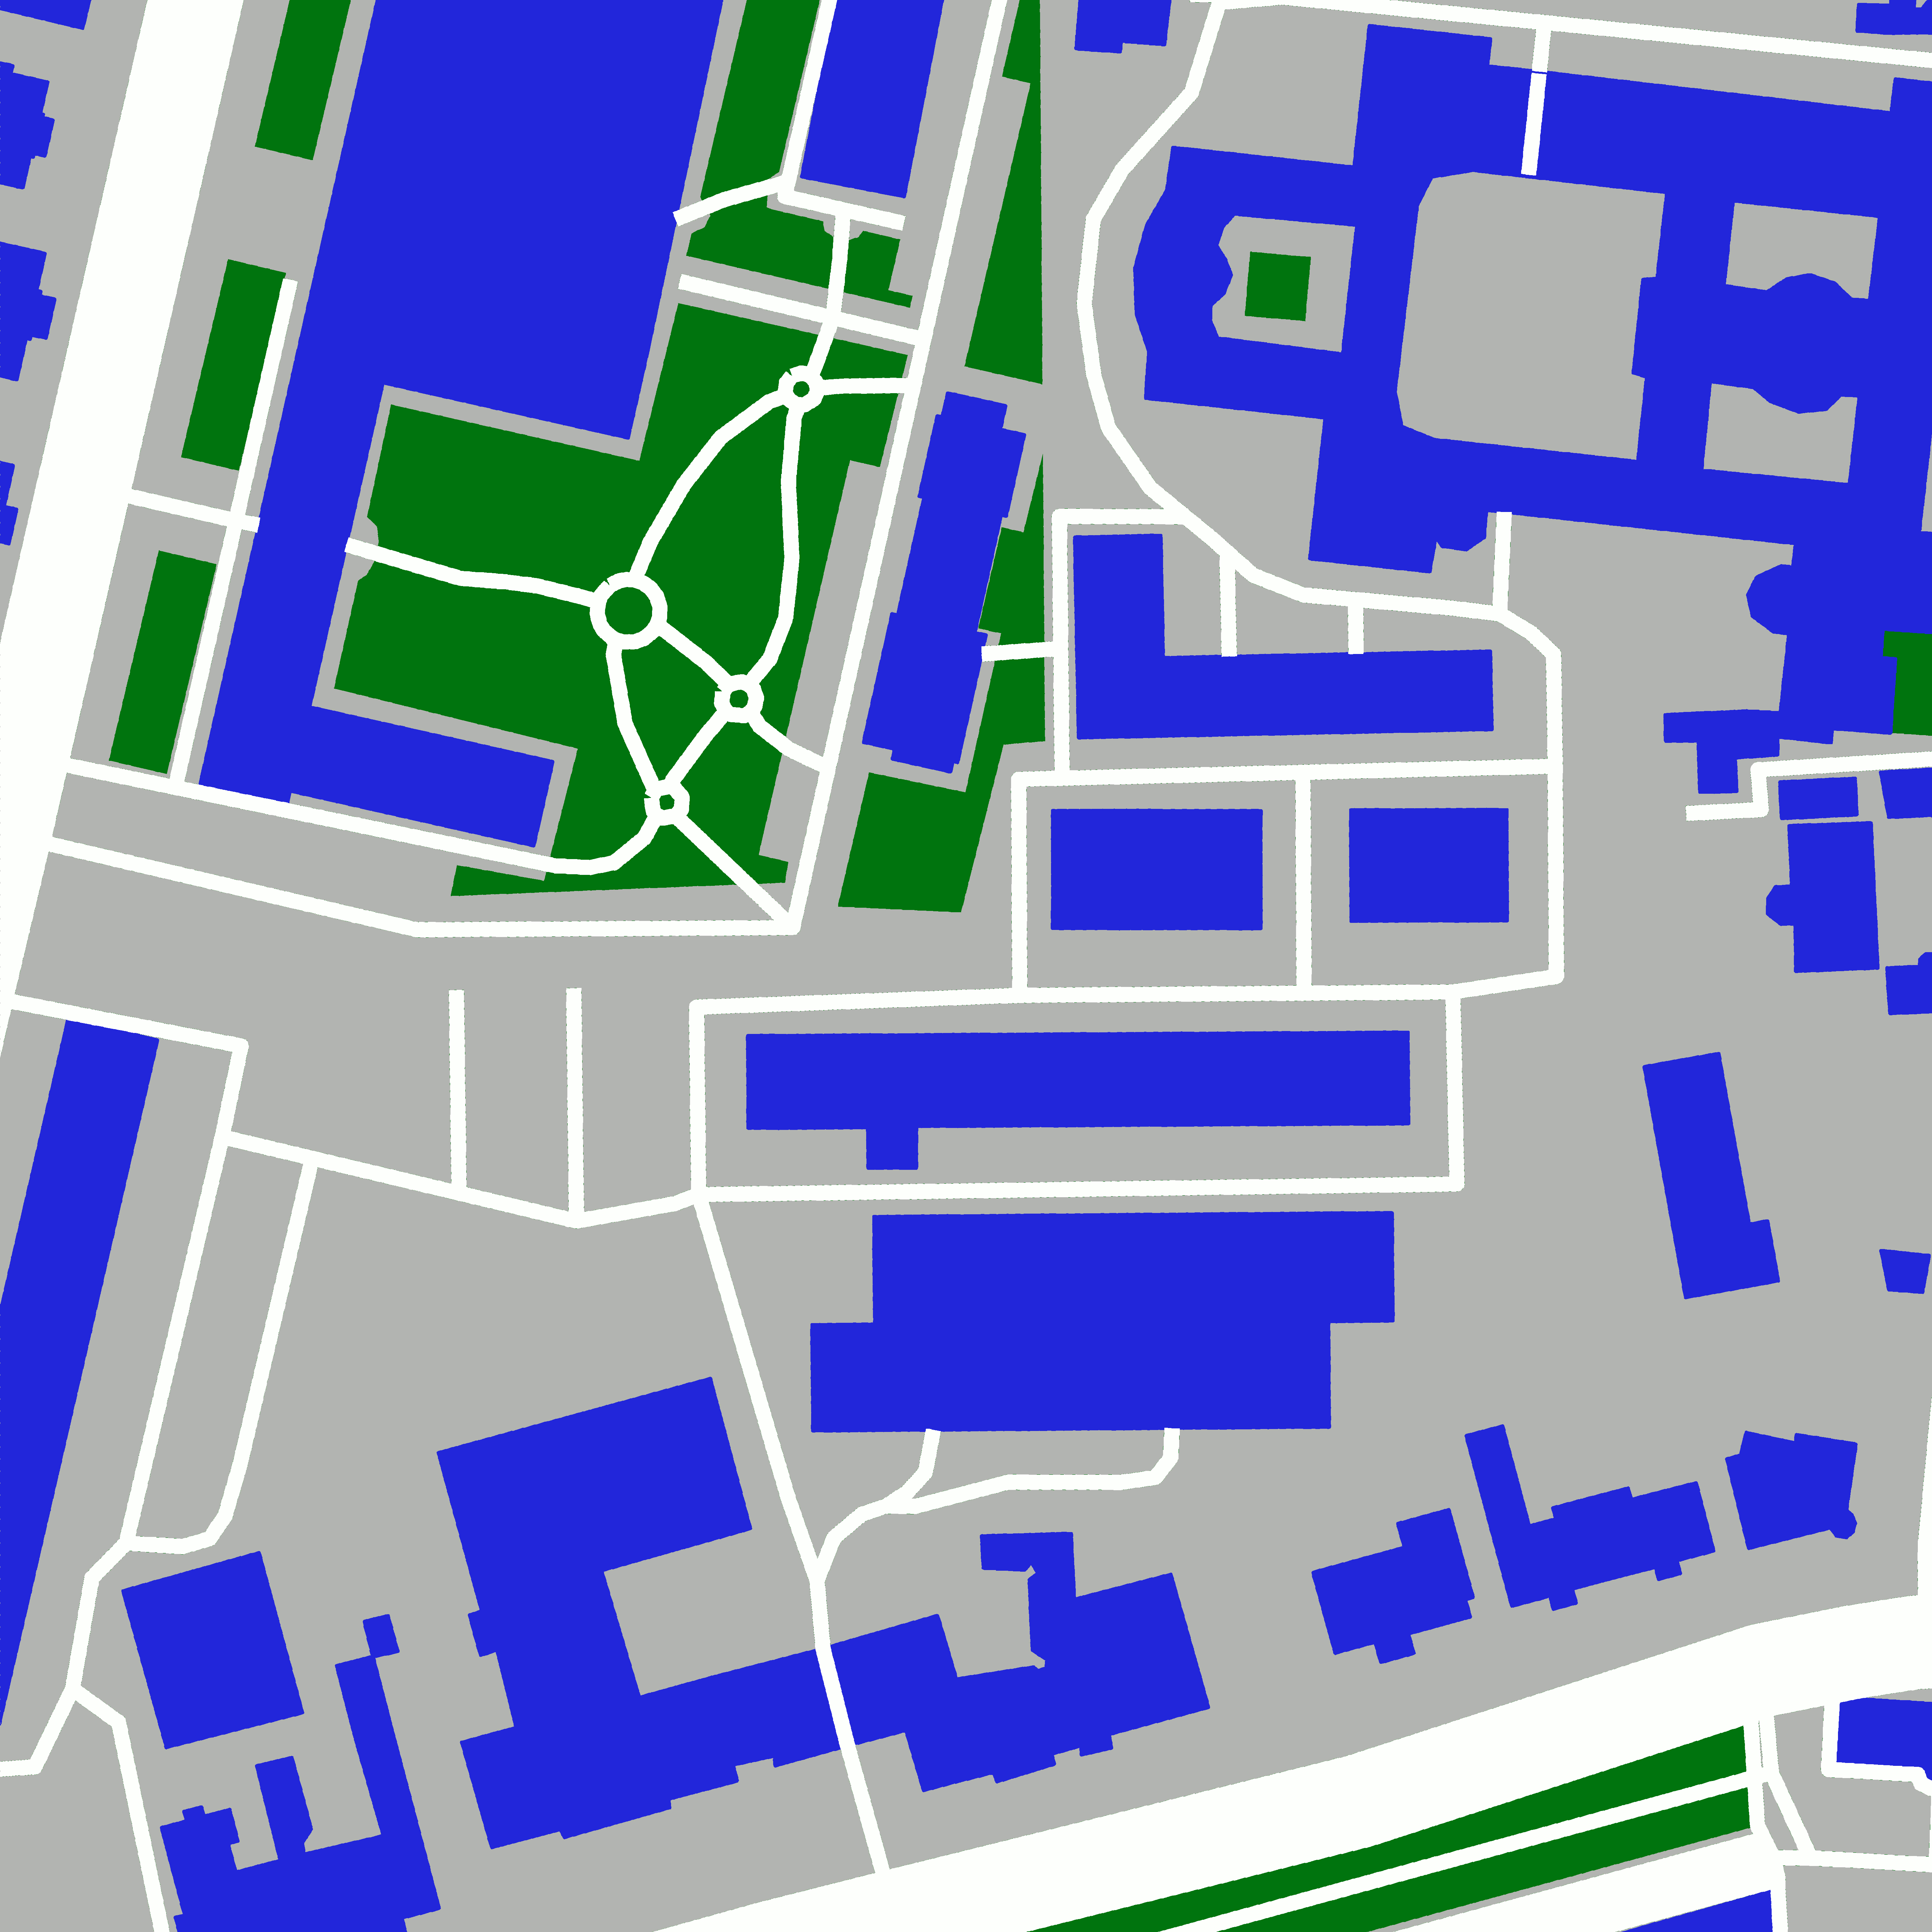
\includegraphics[width=\textwidth]{potsdam_osm_4_12}
    \caption{Données \glsname{OSM}}
\end{subfigure}
\hfill
\begin{subfigure}{0.33\linewidth}
	\includegraphics[width=\textwidth]{potsdam_gt_4_12}
    \caption{Vérité terrain}
\end{subfigure}
\begin{subfigure}{0.49\linewidth}
	\includegraphics[width=\textwidth]{segnet_irrg_potsdam_4_12}
    \caption{Prédiction (SegNet \glssymbol{RVB})}
\end{subfigure}
\hfill
\begin{subfigure}{0.49\linewidth}
	\includegraphics[width=\textwidth]{fusenet_osm_rgb_potsdam_4_12}
    \caption{Prédiction (FuseNet \glssymbol{RVB}+\glsname{OSM})}
\end{subfigure}
\caption[Exemple de segmentation obtenue sur le jeu de données ISPRS Potsdam en incluant la donnée \glsname{OSM}.]{Exemple de segmentation obtenue sur le jeu de données ISPRS Potsdam en incluant la donnée \glsname{OSM}. Les erreurs sur les bâtiments sont grandement réduites.\\\isprslegende}
\label{fig:potsdam_qualitative}
\end{figure}

Les résultats obtenus sur les données de validation de l'\gls{ISPRS} Potsdam sont détaillés dans le~\cref{table_potsdam_results}. Nous calculons les métriques définies dans la~\cref{sec:metriques}, c'est-à-dire le pourcentage global de pixels correctement classés et les scores $F_1$ pour chaque classe, sur la vérité terrain aux bordures érodées.

Comme attendu, l'inclusion de données \gls{OSM} améliore les performances de classification du modèle, notamment pour les routes et les bâtiments qui bénéficient de l'information géographique. En effet, cette information additionnelle permet de supprimer certaines ambiguïtés où un modèle purement optique aurait des difficultés, par exemple pour distinguer un parking au sol et sur un toit, à l'apparence très similaire. Il par ailleurs intéressant de constater que des classes absentes des couches \gls{OSM} bénéficient de cet apport en information, notamment les différents types de végétation et la classe correspondant aux véhicules.
%As could be expected, the inclusion of OSM data improves the semantic labeling performance, with significant improvements on ``road'' and ``building'' classes. This is not surprising considering that those classes already have a representation in the OSM layers which can help disambiguating predictions coming from the optical source. Moreover, OSM data accelerates the training process as it allows the main network to focus on the harder parts of the image. Indeed, OSM data already covers the majority of the roads and the buildings, therefore simplifying the inference of the ``impervious surface'' and ``building'' classes. OSM data also helps discriminating between buildings and roads that have similar textures.

\begin{figure}
\centering
\begin{tabularx}{0.95\textwidth}{c Y Y Y Y Y Y Y}
\glssymbol{RVB} seul &
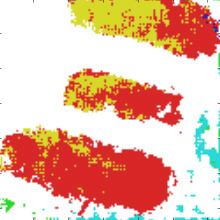
\includegraphics[width=\linewidth]{evolution/rgb_10000} &
\includegraphics[width=\linewidth]{evolution/rgb_20000} &
\includegraphics[width=\linewidth]{evolution/rgb_50000} &
\includegraphics[width=\linewidth]{evolution/rgb_80000} &
\includegraphics[width=\linewidth]{evolution/rgb_120000} &
\glssymbol{RVB} &
\includegraphics[width=\linewidth]{evolution/rgb} \\
\glssymbol{RVB} + \glsname{OSM} &
\includegraphics[width=\linewidth]{evolution/osm_10000} &
\includegraphics[width=\linewidth]{evolution/osm_20000} &
\includegraphics[width=\linewidth]{evolution/osm_50000} &
\includegraphics[width=\linewidth]{evolution/osm_80000} &
\includegraphics[width=\linewidth]{evolution/osm_120000} &
VT &
\includegraphics[width=\linewidth]{evolution/gt} \\
itération & 10 000 & 20 000 & 50 000 & 80 000 & 120 000\\
\end{tabularx}
\caption[Évolution des prédictions de SegNet \glssymbol{RVB} et \glssymbol{RVB}+\glsname{OSM}.]{Évolution des prédictions de SegNet \glssymbol{RVB} et \glssymbol{RVB}+\glsname{OSM}. L'ajout de \glsname{OSM} rend les prédictions visuellement plus structurées.\\
\isprslegende}
\label{fig:training_evolution}
\end{figure}

Par ailleurs, l'intégration des données \gls{OSM} dans l'apprentissage permet d'accélérer la convergence du modèle. Sur le même jeu de données, le modèle SegNet appris par raffinement depuis \gls{OSM} nécessite 25\% d'itérations en moins que le SegNet \gls{RVB} classique et converge vers un meilleur optimal local, avec une fonction de coût à \num{0,39} contre \num{0,45}, pour un même taux de réussite. Enfin, l'inclusion des données \gls{OSM} rend la sortie du réseau visuellement plus cohérente et mieux structurée spatialement, comme illustré dans la~\cref{fig:training_evolution}.

Dans l'ensemble, il apparaît que les \glspl{FCN} sont naturellement bien adaptés pour l'apprentissage multi-modal. En particulier, nous avons montré dans ce chapitre qu'il est possible de tirer profit des multiples sources de données géographiques hétérogènes, aussi bien issues de capteurs que de \glspl{SIG}. Les informations multi-sources permettent d'enrichir les capacités d'inférence de nos modèles aussi bien quantitativement que qualitativement sur les deux jeux de données que nous avons considéré. Enfin, les approches d'apprentissage multi-modal et de fusion de prédictions permettent de faire face à différents types d'obstacles mais semblent bénéfiques dans tous les cas.
%\bibliographystyle{plainnat}
%\bibliography{Chapitre4/Biblio}
\printbibliography
